\chapter{MOTION PRIMITIVE TWEAKING:BIPEDAL WALKING}
\label{chap:walk}
\graphicspath{{BipedWalk/BipedWalkFigs/EPS/}{BipedWalk/BipedWalkFigs/}}


The examples of bouncing ball and mass spring systems explained the idea well, but are too simple for \cms application.
This chapter focus on applications.  
Details are given about how to adapt a motion primitive for  environmental and application specific constraints.
Combination and transitions of motion primitives are discussed in the next chapter.


The motion primitive under study in this chapter is \emph{bipedal walking}, which is a topic of great application value for both the graphic and robotic engineering.
In the past decades, many methods have been applied to the bipedal walking, but still we have not achieved  human bipedal walking ability yet.
The early belief is that bipedal walking in nature is unstable, and many control methods are developed based on trajectory following.
The turning point is the discovery of passive dynamic walking machine, which shows under specific conditions, walking needs not control effort.
This idea leads us to believe that the walking ability is inborn and most problems can be solved by the mechanical structure.

From the perspective of \moit, bipedal walking is  a motion primitive.
In this chapter, the passive walking gait is treated as the template.
Neural Oscillator and Symmetry Control are applied to tweaking the template while maintaining the global and local motor invariants.
This method generate adaptive gaits and stable gaits in real-time.
This process may provide an clear example of application of the \moit idea.




\section{Bipedal Walking Primitives}


bipedal manner means "two feet" (from the Latin bi for "two" and ped for "foot"). 
Types of bipedal movement include walking, running, or hopping, on two appendages (typically legs).
Relatively few modern species are habitual bipeds whose normal method of locomotion is two-legged. 
Within mammals, habitual bipedalism has evolved four times, with the macropods, kangaroo mice, springhare and homininan apes. 

A larger number of modern species are capable of bipedal movement for a short time in exceptional circumstances.
Several non-archosaurian lizard species move bipedally when running, usually to escape from threats. 
Many animals rear up on their hind legs whilst fighting or copulating. 
There are two main types of bipedal locomotion: macropods, some smaller birds[citation needed], and heteromyid rodensts move by hopping on both legs simultaneously; other groups, including apes and larger birds, walk or run by moving one leg at a time.

Bipedalism evolved well before the large human brain or the development of stone tools.
Recent evidence regarding modern human sexual dimorphism (physical differences between men and women) in the lumbar spine has been seen in pre-modern primates such as Australopithecus africanus. 





Walking is characterized by an "inverted pendulum" movement in which the body vaults over a stiff leg with each step.
In humans, walking is composed of several separate processes:
Vaulting over a stiff stance leg
Passive ballistic movement of the swing leg
A short 'push' from the ankle prior to toe-off, propelling the swing leg
Rotation of the hips about the axis of the spine, to increase stride length
Rotation of the hips about the horizontal axis to improve balance during stance

In \moit, walking is treated as an independent motion pattern.
For human,the walking dynamic can be simplified.


\begin{figure}[!htbp]
  \begin{center}
    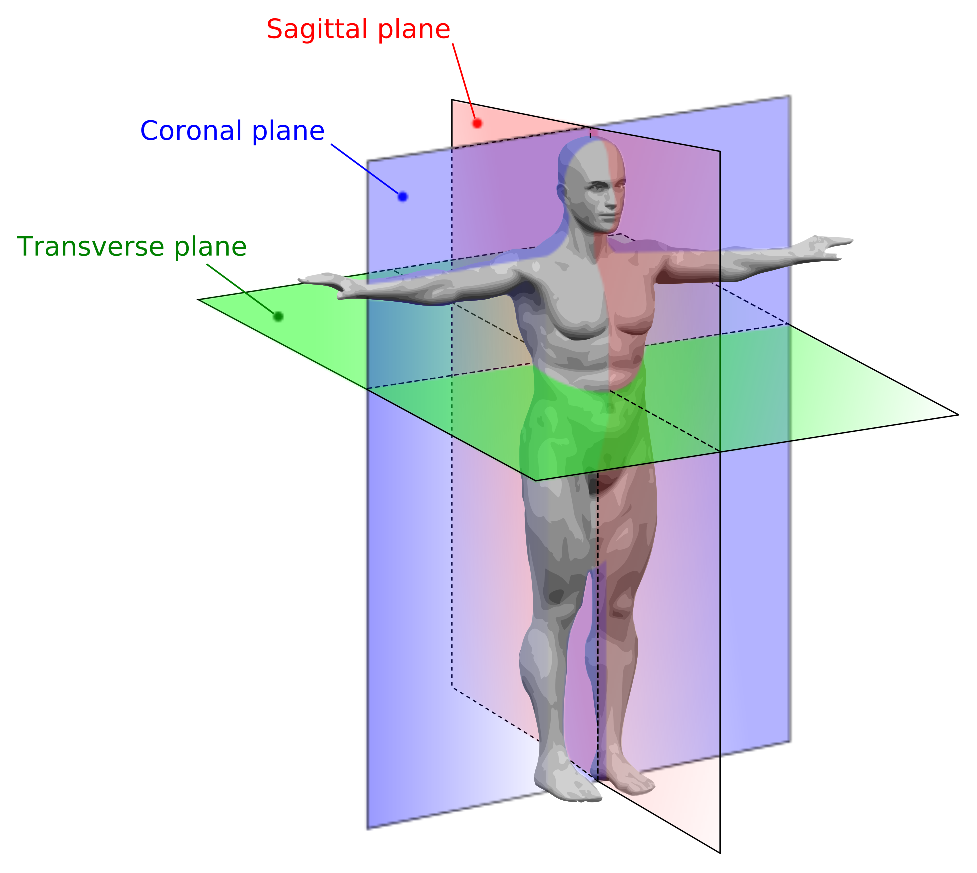
\includegraphics[width=0.7\textwidth]{spahittalPlae}
    \caption{SpahittaPlane}
    \label{fig:passivekneewalker}
\end{center}
\end{figure}

As shown in Figure~\ref{fig:passivekneewalker}, motion is projected into three spaces:the sagittal plane, coronal plane and transverse plane.
For bipedal walking,
 yaw and roll motion are relative small and usually treated as secondary motion or totally neglected,  main motion happens in the \emph{sagittal plane}.




This chapter focuses on the motions in sagittal plane, and  \dof s in coronal plane and transverse plane are discussed in Chapter~\ref{chap:highdor}.
More \dof s will introduce perturbations to our model, but will not change the basic motion characteristics and adaptation tendency.
They will make the ``symmetry'' not so perfect and may cause confusions in explaining the idea. thus the discussion is delayed.




\subsection*{Dynamics}

The simplified walking model is shown in Figure~\ref{fig:passivekneewalker}.

\begin{figure}[!htbp]
  \begin{center}
    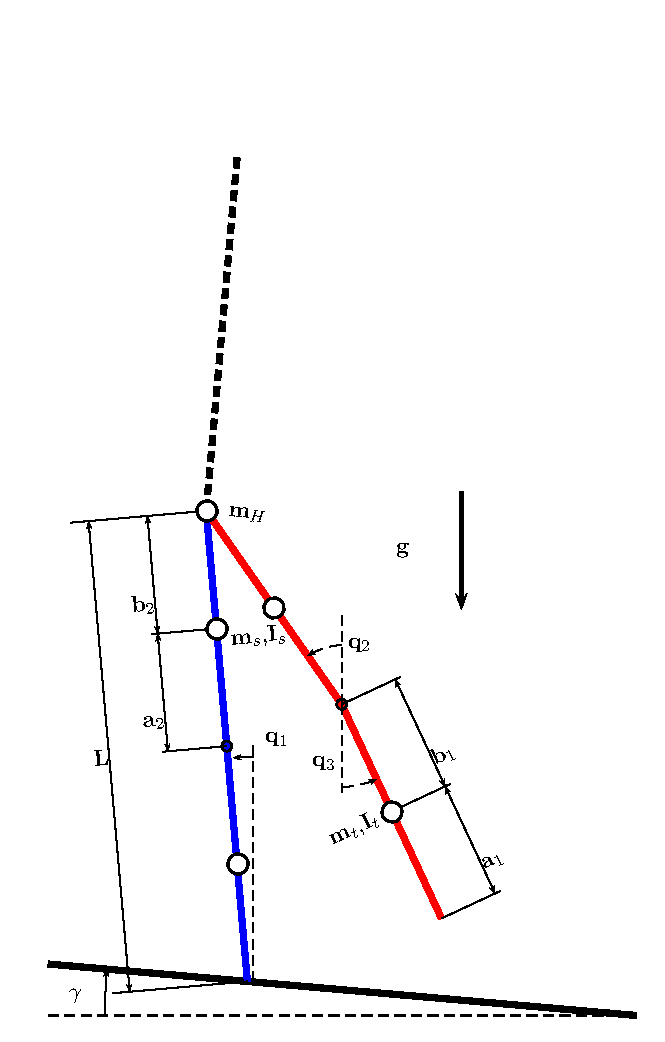
\includegraphics[width=0.7\textwidth]{PWI}
    \caption{A Passive Walking Model with Knee}
    \label{fig:}
  \end{center}
\end{figure}
The walking model of Figure~\ref{fig:passivekneewalker} is based on rigid body dynamics.
The supporting leg is kept straight.$L$ is the length of the leg,and $q_1$ is the angle of the supporting leg,
$m_t$ and $m_s$ are the mass of the shank and thigh,
$q_1$,$q_2$ are the relative angles.
$b_1,a_1$ and $b_2,a_2$ describe the relative position of gravity center.
$m_h$ represents the body and hip mass.






Like the bouncing ball system, this system is hybrid\citep{ames2006categorical} and includes continuous and discrete dynamics.
Passive walking with knees includes four phases\citep{Chen2007}.
\begin{itemize}
\HiItem{Free Swing Phase}
The support leg (the blue one) is kept straight,during this phase the knee of the swing leg is bended, the thigh and shank swing freely.
\HiItem{Knee Strike Phase}
The knee joint of the swing leg has a limit.
When the knee angle reaches the limit,a collision happens.
After the collision, the swing leg is kept straight.
\HiItem{Knee Lock Swing Phase}
During this swing phase, both the swing and support leg are kept straight.
\HiItem{Heel Strike Phase}
When the heel of the swing leg hits the ground, a collision happens and after that the swing and support legs are switched.
\end{itemize}

Figure~\ref{fig:fwalkingphase} shows the the gaits of four phases.
\begin{figure}[!htbp]
  \begin{center}
      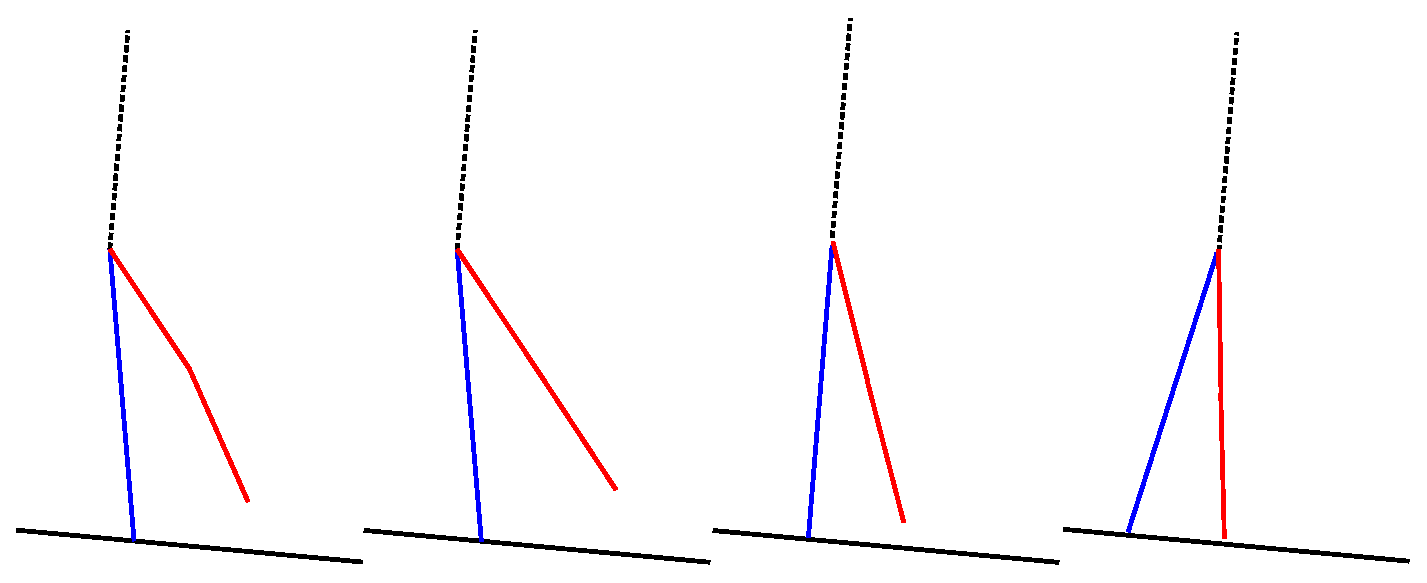
\includegraphics[width=0.7\textwidth]{Fourphase}
    \caption{The four phases in Walking}
    \label{fig:fwalkingphase}
\end{center}
\end{figure}





\begin{itemize}
\HiItem{Flying Phases}
For both the free and locked knee swing phases are described by the continuous dynamics.
Both equations are in the form of Equation~\ref{eq:flyequation}.
\begin{equation}
\label{eq:flyequation}
M(\mathbf{q}) \ddot{\mathbf{q}} + C(\mathbf{q,\qd})\dot{\mathbf{q}} + N(\mathbf{q}) = 0
\end{equation}
where $q=[q_1,q_2,q_3]$,$\qd=[\dot{q_1},\dot{q_2},\dot{q_3}]$,$M$ is the initial mass matrix, $C$ and $N$ are the centrifugal force matrix and gravity respectively. 
For Free Swing Phase,  $M$ and $C$ are $3$ by $3$ Matrix, $N$ is $3$ by $1$ vector.
for Knee Lock Phase, $M$ and $C$ are $2$ by $2$ Matrix, $N$ is $2$ by $1$ vector.
Put into the standard form, define $\state=[q,\qd]$, Equation~\ref{eq:flyequation} is transformed into Equation~\ref{eq:stateformpw}
Then the function is in the form.
\begin{equation}
\label{eq:stateformpw}
\dot{\state}=
-\left[ 
\begin{array}{cc}
\mathbf{1} &0\\
0 &M 
\end{array}
\right]^{-1}
\left[ 
\begin{array}{cc}
0 &\mathbf{1}\\
0 &C 
\end{array}
\right]\state
-\left[ 
\begin{array}{c}
\mathbf{0}\\
 N 
\end{array}
\right]
\end{equation}

\HiItem{The Strike Phases}
The knee strike and heel strike phases are modelled based on discrete dynamics.
collision equations are developed based on momentum preserving principle.
both collision equations are in the form of Equation~\ref{eq:collidequ}.
\begin{equation}
\label{eq:collidequ}
J^{+}\dot{\mathbf{q}}^{+} = J^{-}\dot{\mathbf{q}}^{-}
\end{equation}

where $J$ is the matrix of angular momentum inertia, the superscripts~$+,-$ represent those after and before collision.
For Knees Strike,$J^-$ is a 3 by 2 Matrix, $J^+$ is 2 by 2 Matrix;
For Heel Strike, both $J^{+,-}$ are 2 by 2 Matrix.
\end{itemize}
Dynamic equations are developed based on Lagrange Mechanics~\citep{Goldstein2002}.
For details of calculating the dynamic equation, please refer to \citep{Chen2007}
For the components of each matrix, please refer to the appendix.









\begin{figure}[!htbp]
  \begin{center}
    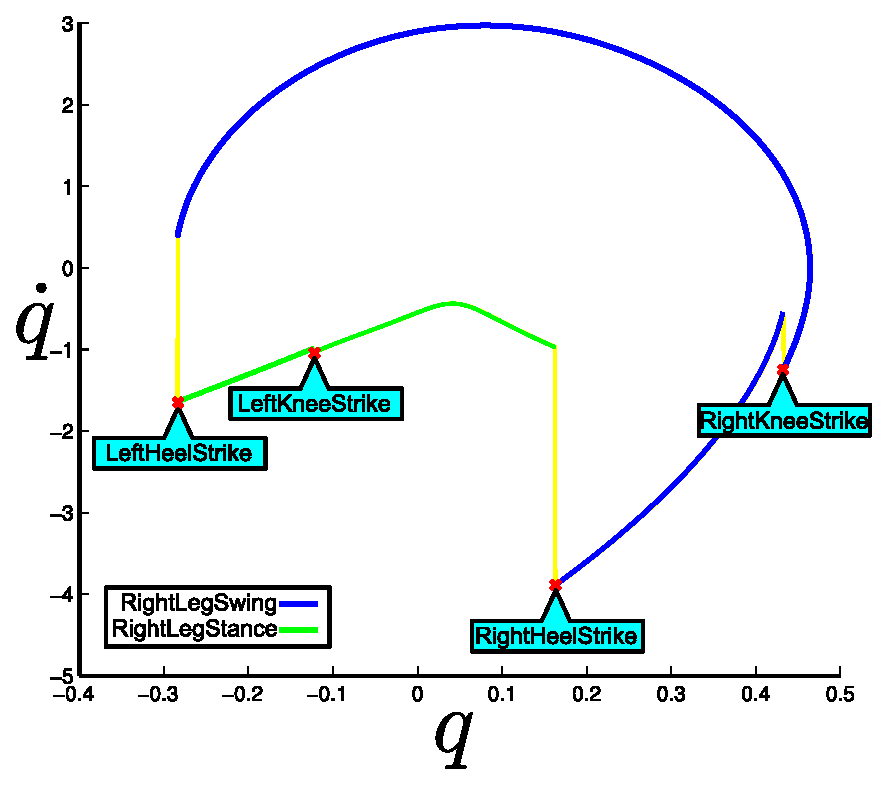
\includegraphics[width=0.7\textwidth]{walk_cycle_index}
    \caption{Four Phases Markered on a Walking Cycle}
    \label{fig:phasesmaker}
\end{center}
\end{figure}
With special initial conditions, the passive walker can walk down the slope with a stable gait.
On the phase plot,  a limit cycle emerge. 
Figure ~\ref{fig:phasesmaker} shows the phase plot of one thigh for a stable walking cycle.
where the four phases are marked. 

In theory, the generalized coordinates for walking have $4$ degrees of freedom, with angle for shank and thigh for each leg.
Thus the state space is $8$ dimension, which is not possible to draw in a $2D$ picture.
But since motions of the two legs are almost the same, so showing one motion is enough, the state space is reduced to $4$ dimension.
In the further analysis, we show that knee motion is not very important, the motion of the thigh captures the most valuable motion.
Thus we only draw the phase plot of the thigh of one leg.
Figure ~\ref{fig:phasesmaker} only shows the motion right leg.
the green plot shows the stance phase, when the right leg is supporting the body.
the blue parts shows the swing phase, when the the right is swing and the left leg is supporting.
The yellow lines marker the $4$ collision events during walking.
Note that during collision, the walking dynamic is discontinuous, the speed of walking is changed suddenly without changing the position.
this means the yellow segments are not on the limit cycle, only the two ends are, if the walker starts from the state in the middle of the yellow segment, it will fall.











\section{Global Motor Control and Adaptive Gaits}
The Passive Dynamic Walker exhibits natural looking gait, but the walking motion is not stable.
In \moit, the repetitive walking motion suggests that the natural walking dynamic forms a limit cycle.
Human utilize the limit cycle for walking, which results in high energy efficiency.

To overcome the fragile stability, \cpg is applied with the hope to make the walking more stable through entrainment.
Experiments have shown that stability is enhanced and different perturbations result in varied and natural looking responsive motions.




\subsection{Entrainment}
For walking, only one neural oscillator is applied to maintain the stability of limit cycle.
The output of neural oscillator worked as torque applied at hip angel (angle between the two thighs).
The dynamics are shown in Equation~\ref{eq:neuralwalk}
\begin{equation}
\label{eq:neuralwalk}
M(\mathbf{q}) \ddot{\mathbf{q}} + C(\mathbf{q,\qd})\dot{\mathbf{q}} + N(\mathbf{q}) = D\uout
\end{equation}
For the knee lock phase $D=[1,-1]^T$.
For the knee free phase, $D=[1,-1,0]^T$(acting on the difference between the two thighs, not effect the knee)

the input signal is the hip angle,
we have 
\[
	\uin=\hin(q_1-q_2)
\]





\begin{figure}[!htbp]
  \begin{center}
    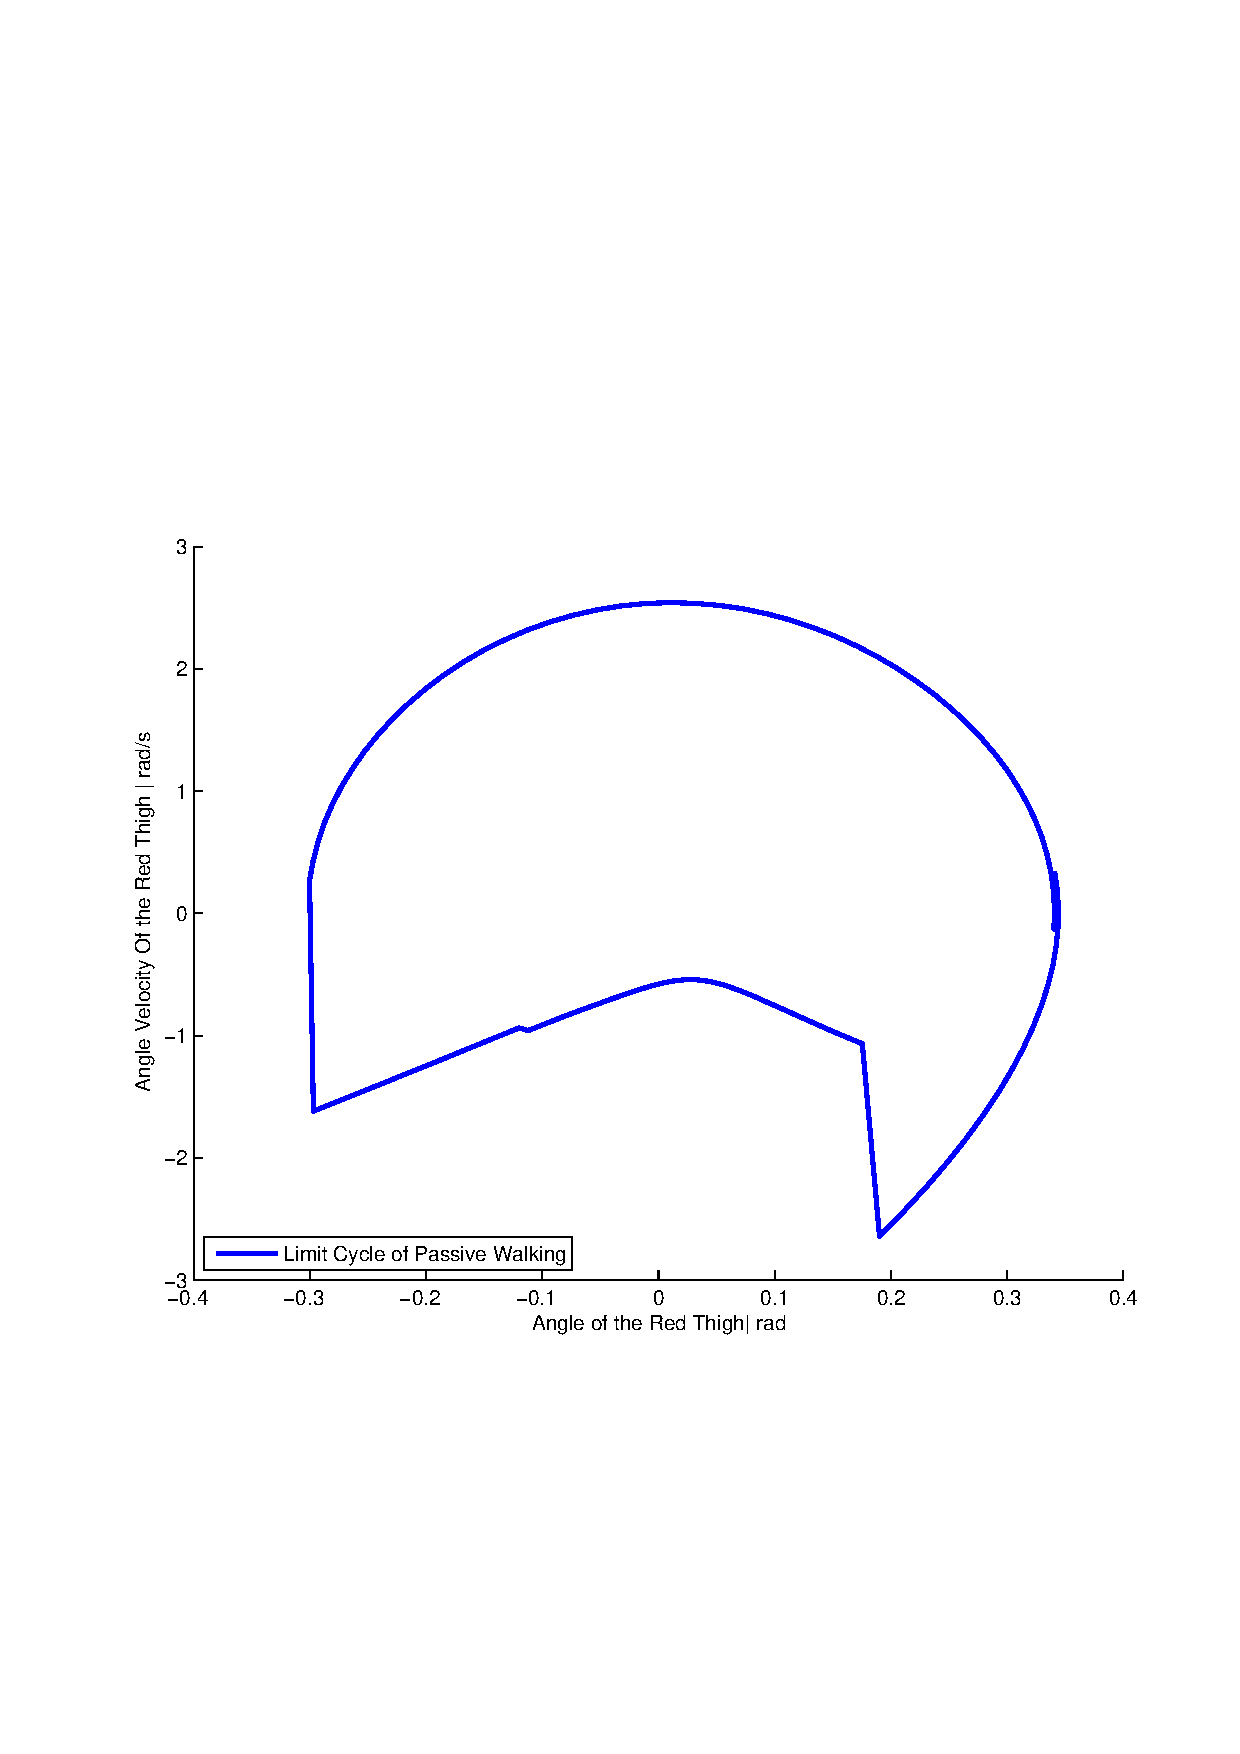
\includegraphics[width=0.7\textwidth]{PassiveWalkingLimitCycle}
    \caption{Limit Circle And Different Phase in Passive Walking}
    \label{fig:passivegaitlimitcycle}
\end{center}
\end{figure}


\begin{figure}[!htbp]
  \begin{center}
      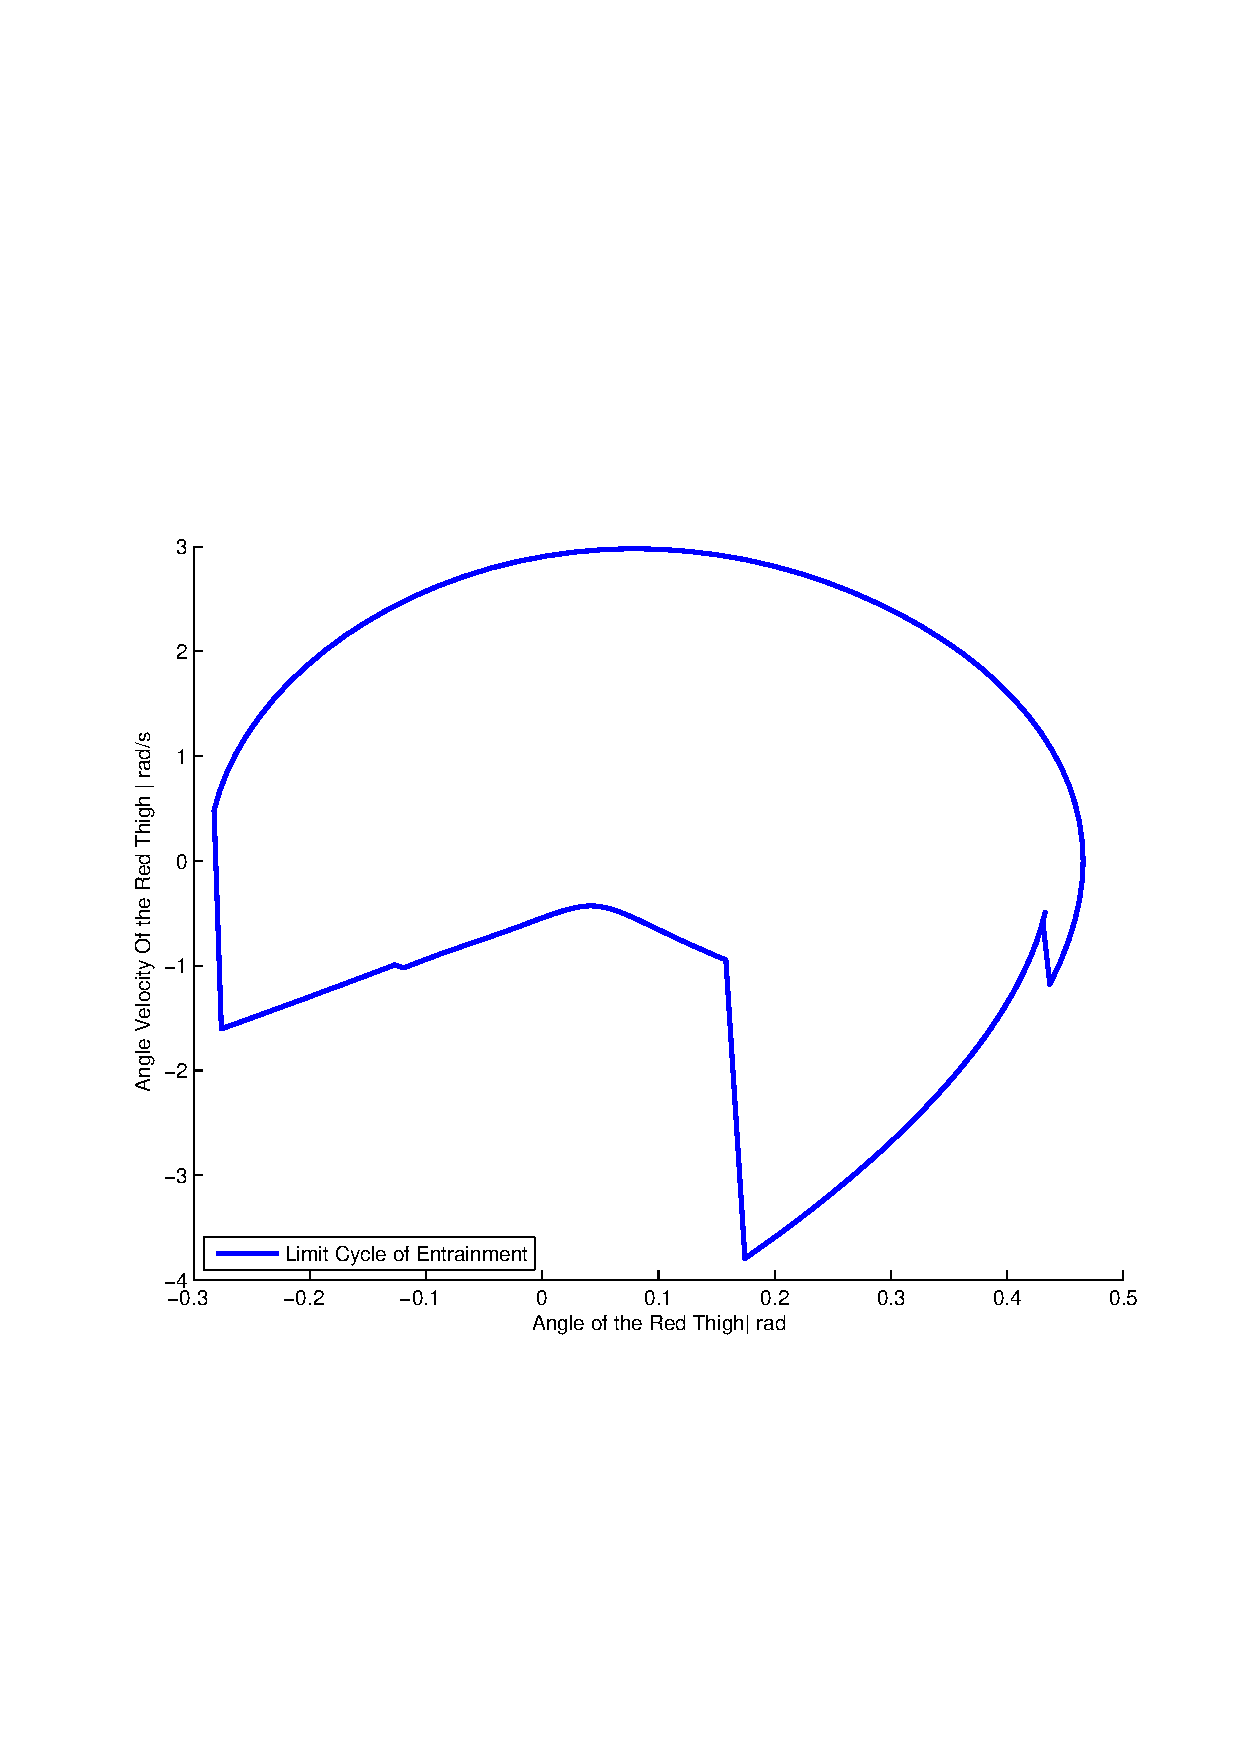
\includegraphics[width=0.7\textwidth]{NeuralWalkingLimitCycle}
    \caption{The gait with neural controller}
    \label{fig:entrainmentgaitlimitcyle}
\end{center}
\end{figure}
when the drive force is small, the limit cycle of entrainment system is similar to original passive one.
Both limit cycles are shown in Figure~\ref{fig:passivegaitlimitcycle} and Figure~\ref{fig:entrainmentgaitlimitcyle}.
Walking gaits are shown in Figure~\ref{fig:entrainmentgait} and Figure~\ref{fig:passivegait}.
Both figures are sampled by the same time interval, the controlled gait looks a little sparser, which means the controlled gait is a bit quicker. 




\begin{figure}[!htbp]
  \begin{center}
     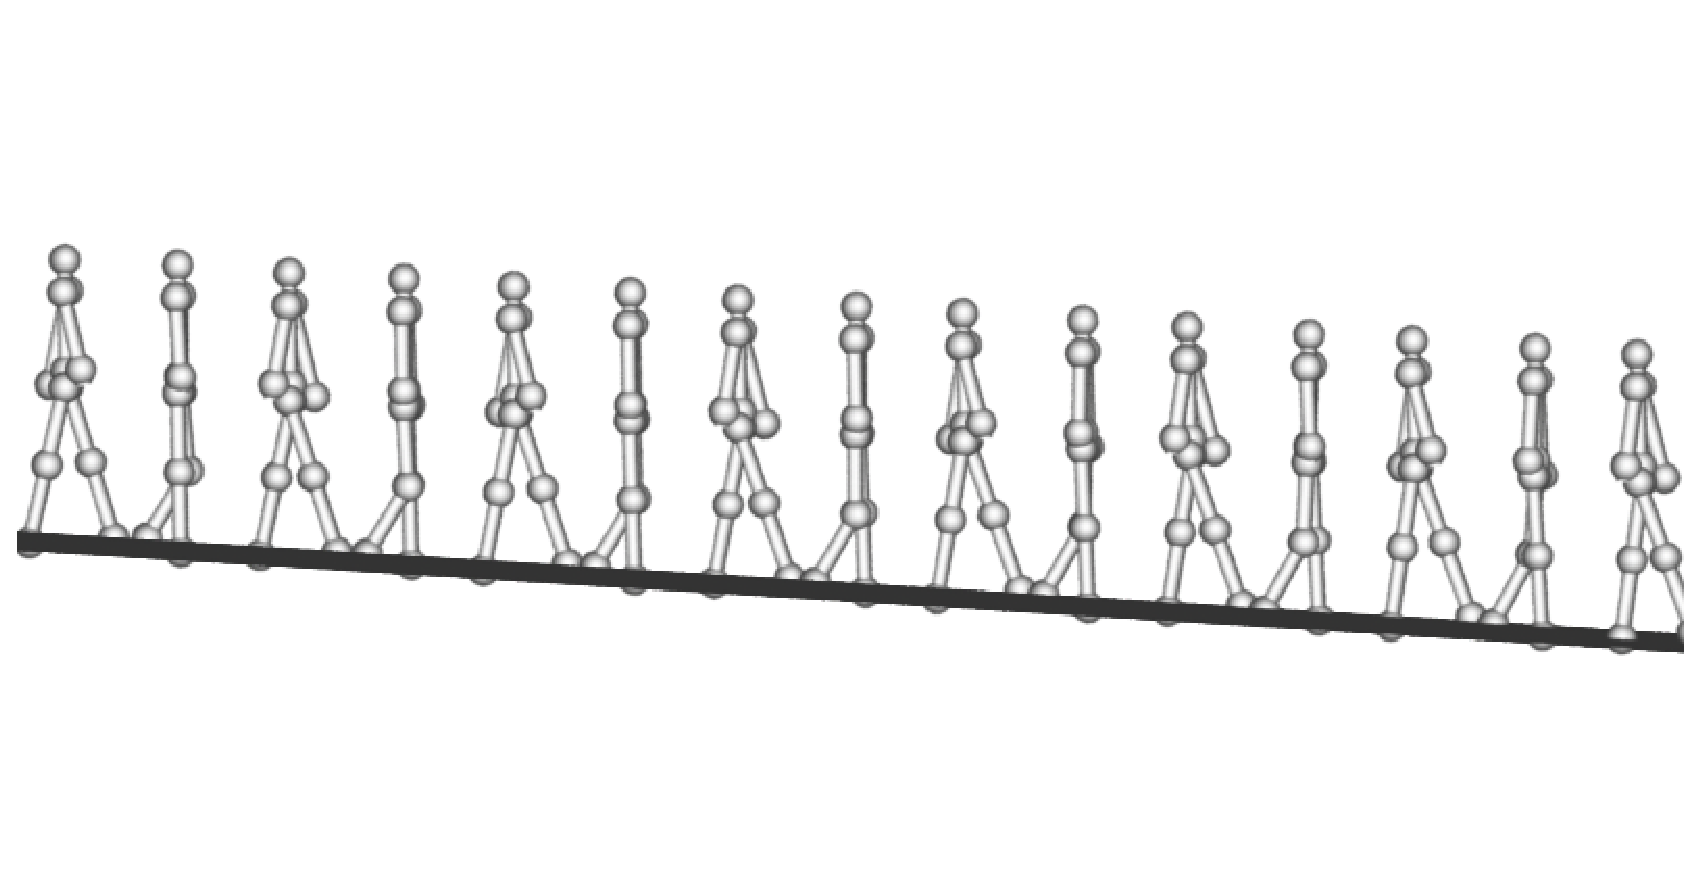
\includegraphics[width=0.7\textwidth]{PassiveGait}
    \caption{The Passive Walking Gait}
    \label{fig:passivegait}
\end{center}
\end{figure}

\begin{figure}[!htbp]
  \begin{center}
     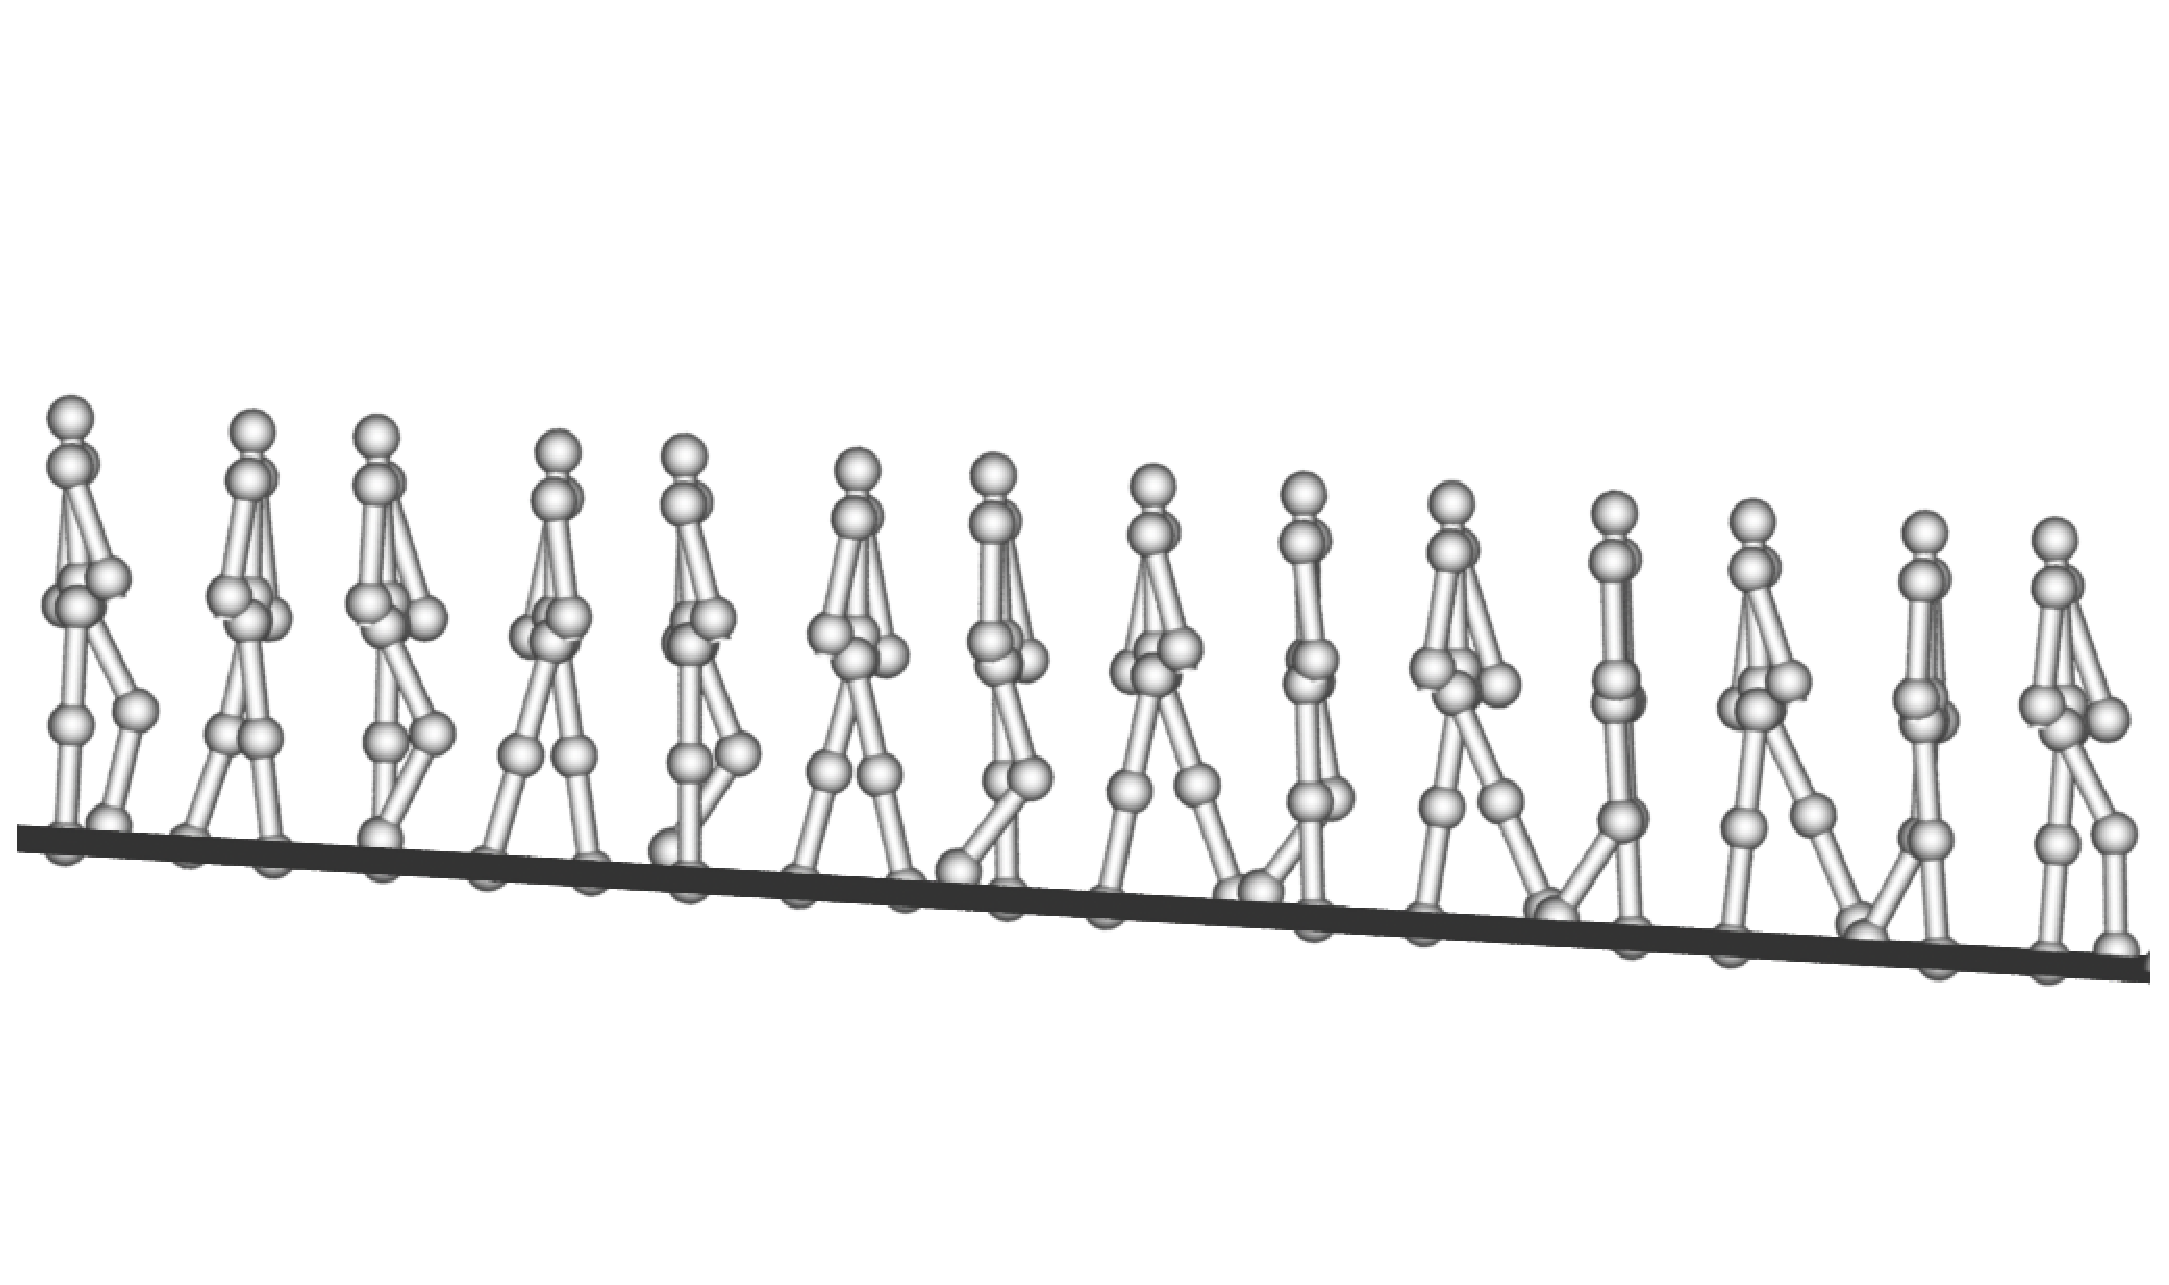
\includegraphics[width=0.7\textwidth]{neuralWalk}
    \caption{Passive Walking with Neural Control}
    \label{fig:entrainmentgait}
\end{center}
\end{figure}

By comparing the limit cycle and the walking gaits, we find out that the controlled gait and passive gait are quite similar.
The controlled gaits are a bit faster and the step size is a slightly bigger.
To a human observing eye, the two gaits are almost the same, both are natural very hard to detect control effort.
But the dynamics has been changed greatly, especially the stability.



\subsubsection*{Structural Stability}
Entrainment  boosts structural stability of walking. 
The passive walking can not be maintained on plane, structure perturbation from slope angle violate the topology, limit cycle does not exist any more.


When passive walker walks on a plane,the step-size decreases every step.
After several steps, the walker will stop or fall over,as shown in Figure~\ref{fig:passivegaitplane}.

After coupling with neural oscillator, the  walker maintain the gait with a small step size,as shown in Figure~\ref{fig:neuralwalkinggait}.
To maintain the energy efficient property of natural motion, $\uout$ is limited to small, thus maintain a small step size,as shown in Figure~\ref{fig:entrainmentLimitCycleOnPlane}.

\begin{figure}[!htbp]
  \begin{center}
    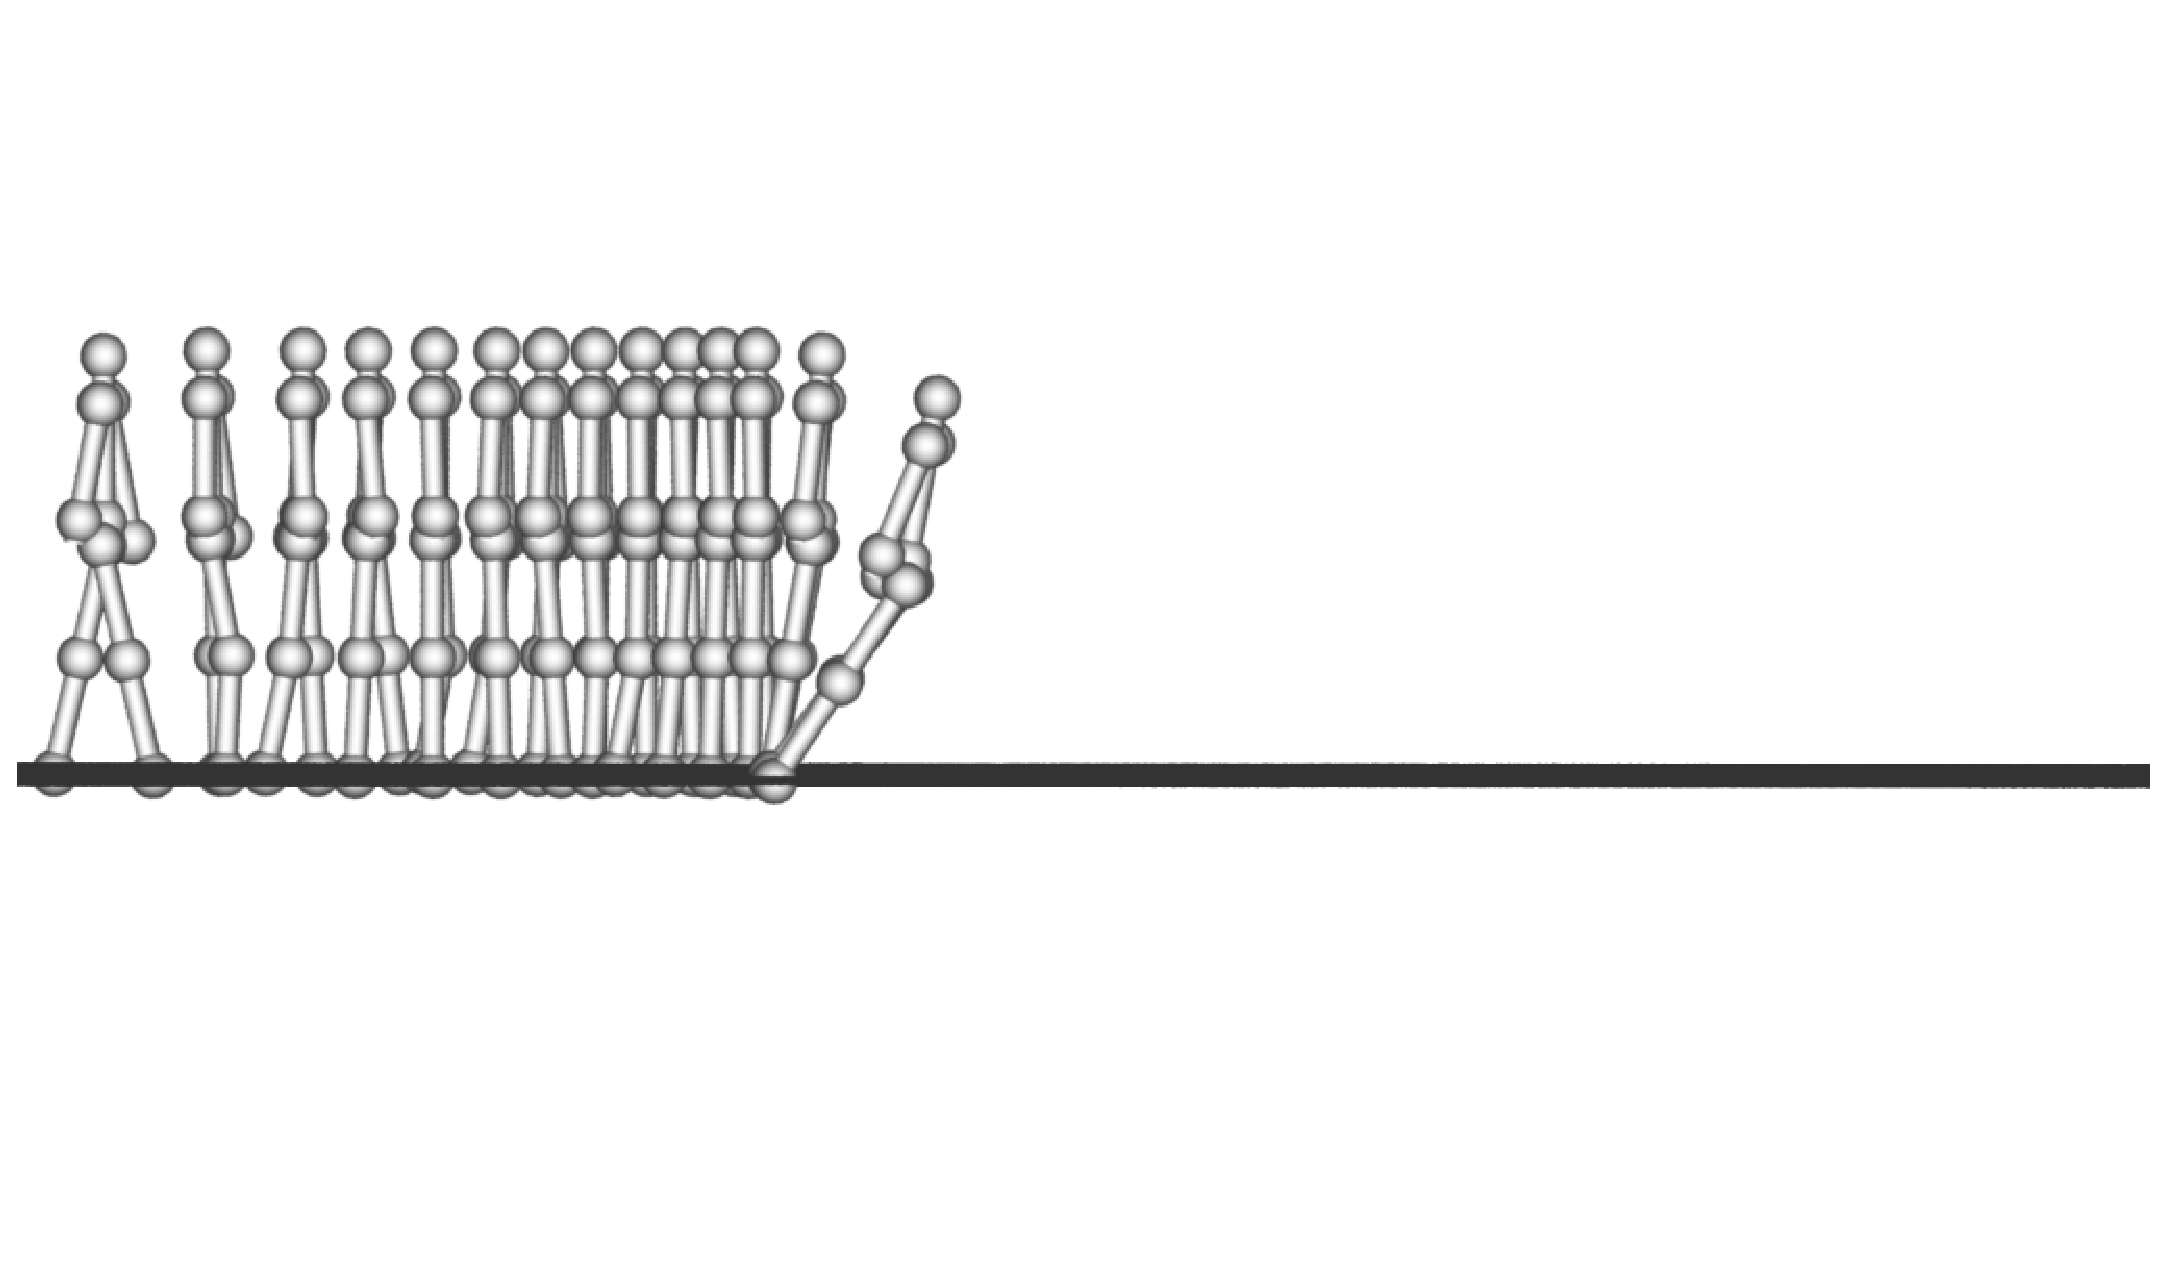
\includegraphics[width=0.7\textwidth]{PassiveOnPlane}
    \caption{Passive On Plain}
    \label{fig:passivegaitplane}
\end{center}
\end{figure}

\begin{figure}[!htbp]
  \begin{center}
     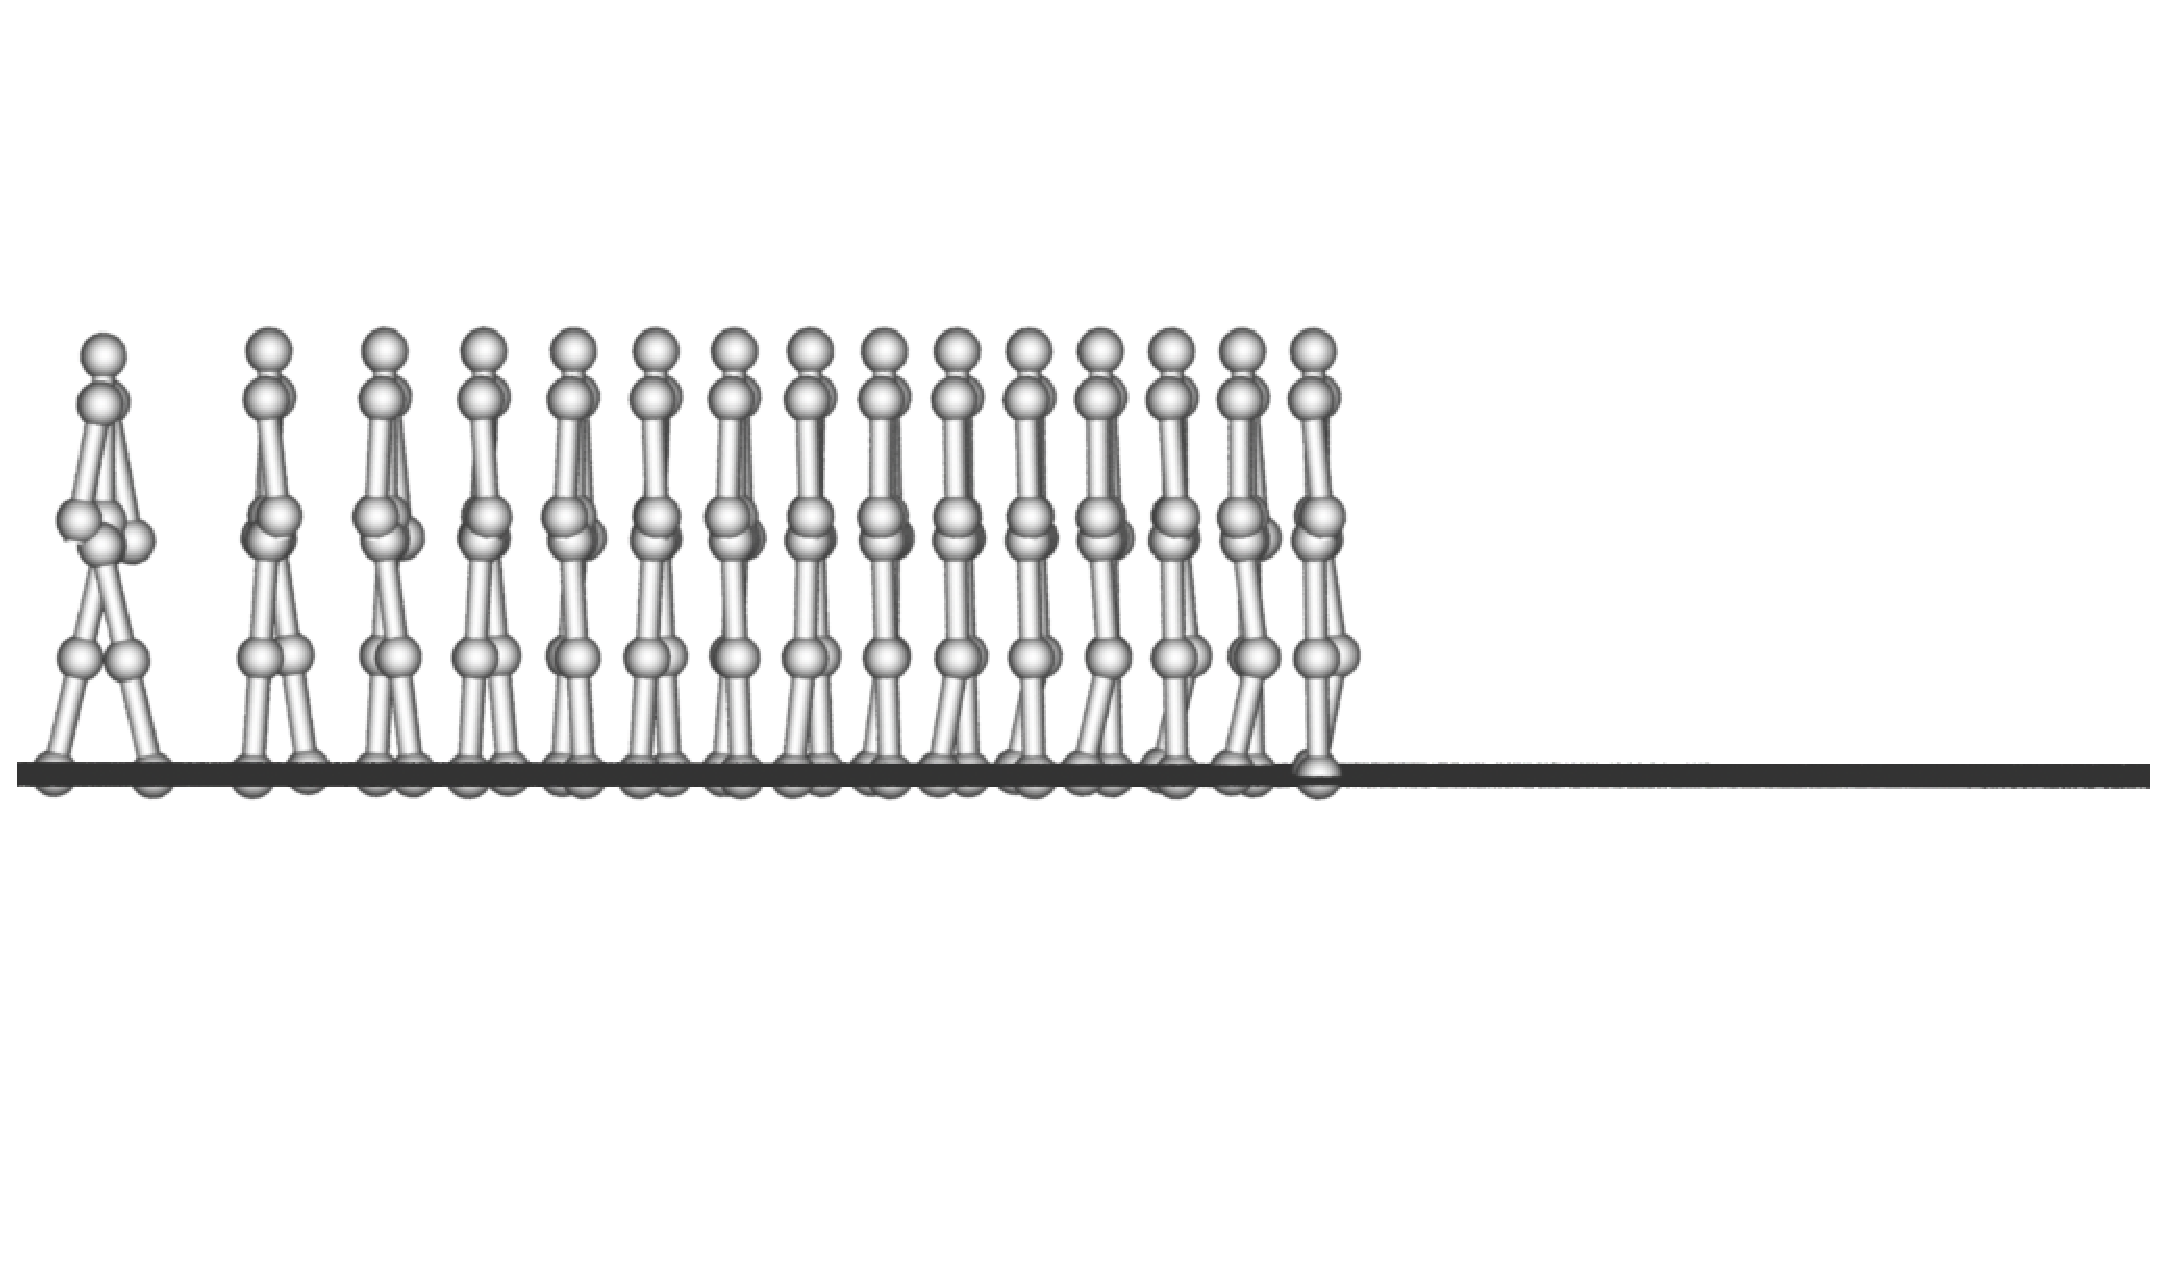
\includegraphics[width=0.7\textwidth]{NeuralWalkingPlane}
    \caption{Entraint Gait On Plane}
    \label{fig:neuralwalkinggait}
\end{center}
\end{figure}

\begin{figure}[!htbp]
  \begin{center}
      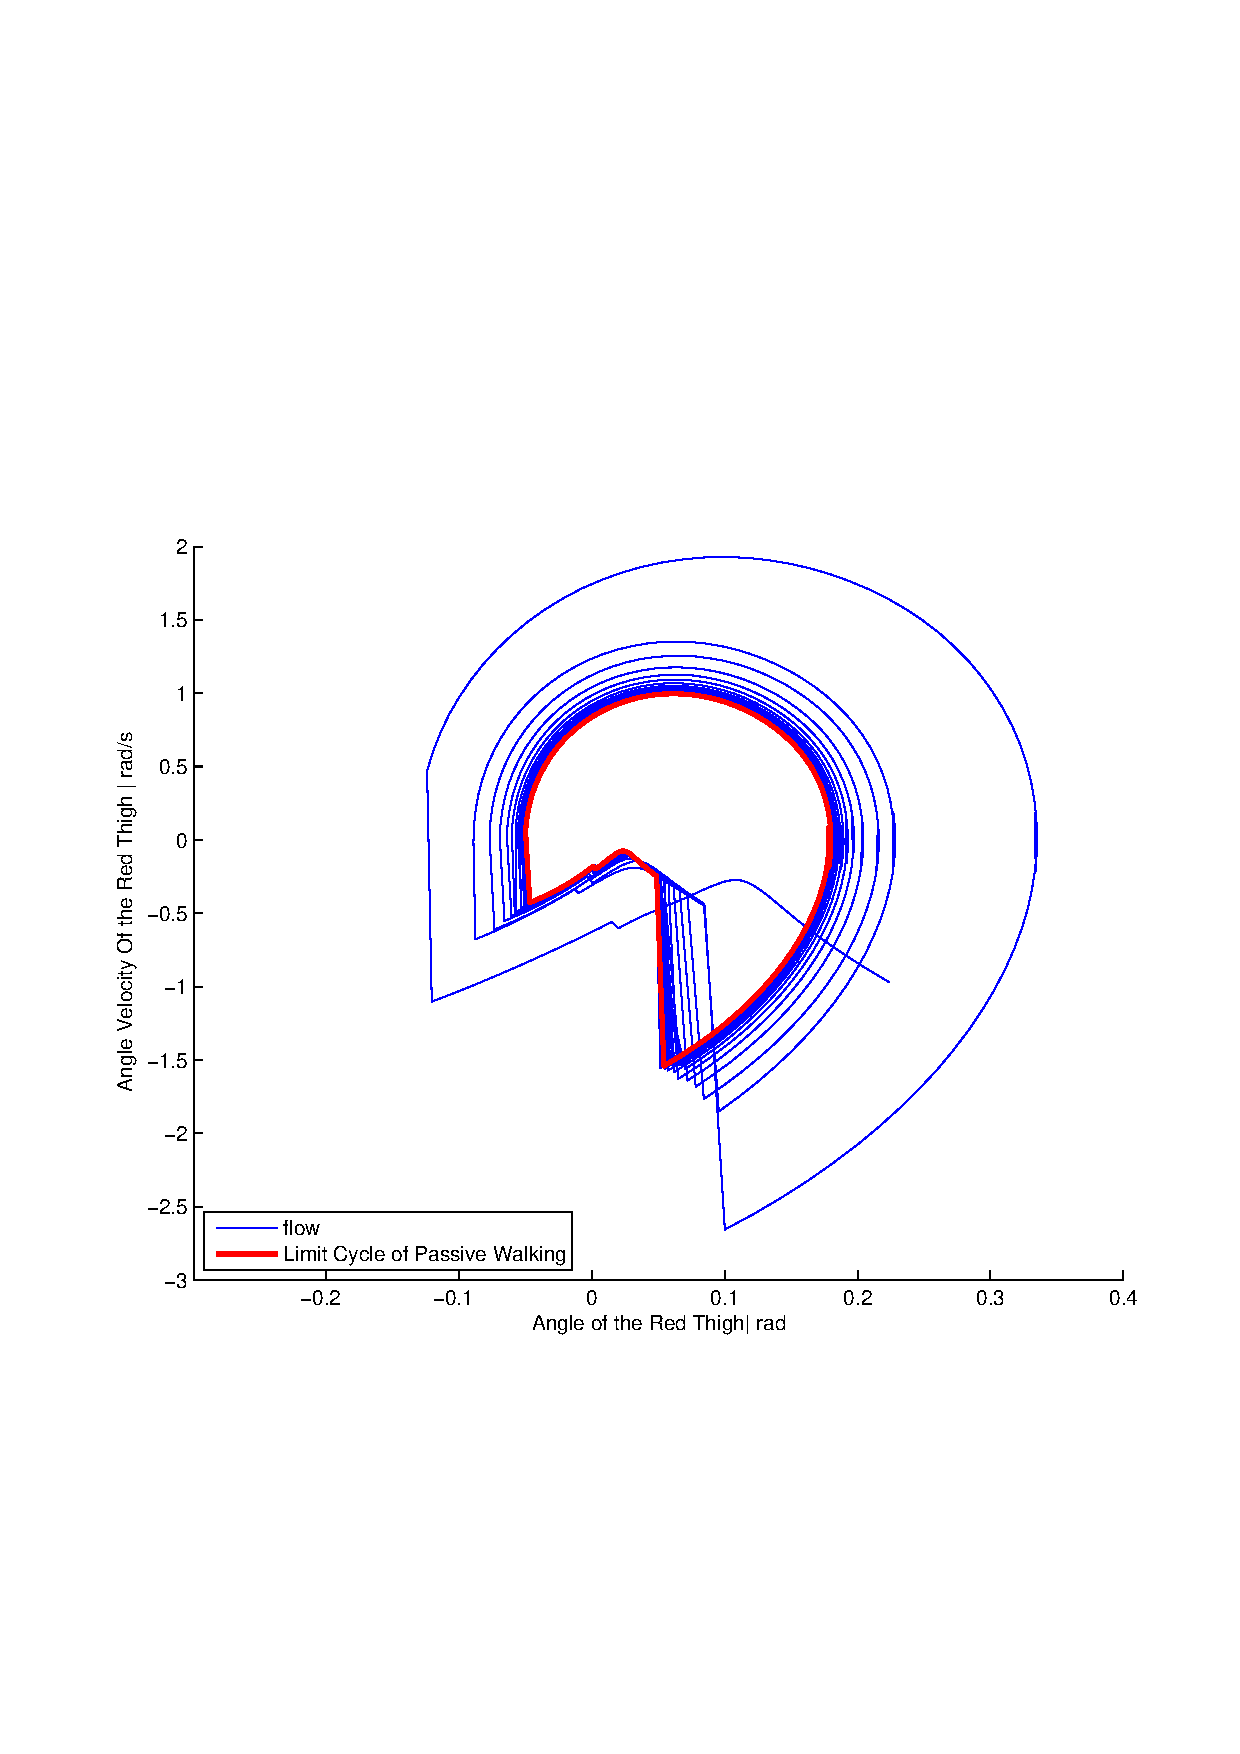
\includegraphics[width=0.7\textwidth]{NeuralPlaneCycle}
    \caption{Limit Cycle of entrainment gait on plane}
    \label{fig:entrainmentLimitCycleOnPlane}
\end{center}
\end{figure}

Figure~\ref{fig:entrainmentLimitCycleOnPlane},the walking cycle is kept shrinking overtime, this results a gaits of walking to stop intention. 
But after several steps, the walking gaits reach a limit cycle (shown in red). 
The new walking limit cycle is of a smaller size, which means a smaller step.


\subsubsection*{Area of Basin of Attraction}
Another measurement for stability is to size of the basin of attraction.
Passive walking is fragile, which means the basin of attraction is very narrow.
If the walker is pushed, it will fall.

Entrainment greatly enlarged the basin of attraction of the walking limit cycle.
For Figure~\ref{fig:entrainmentLimitCycleOnPlane}, the initial position is far from the limit cycle, this shows that the basin of attraction has been enlarged.

A better test is to push or pull the walking character.
When push and pull is applied to the character, the state is moved away from the limit cycle.
The harder the push or the pull is, the further it moves away.
The gaits of  pushed or pulled walking shown in Figure~\ref{fig:PushGait} and Figure~\ref{fig:PullGait}.
For both cases, the characters start walking with normal stable gaits.
When the character is pushed forward, the character will take a big step and then slowly return to the normal step;
when the character is pulled backward, the character will take a smaller step or even step backwards for one or two step, and then gradually return to normal walking gait.


\begin{figure}[!htbp]
  \begin{center}
      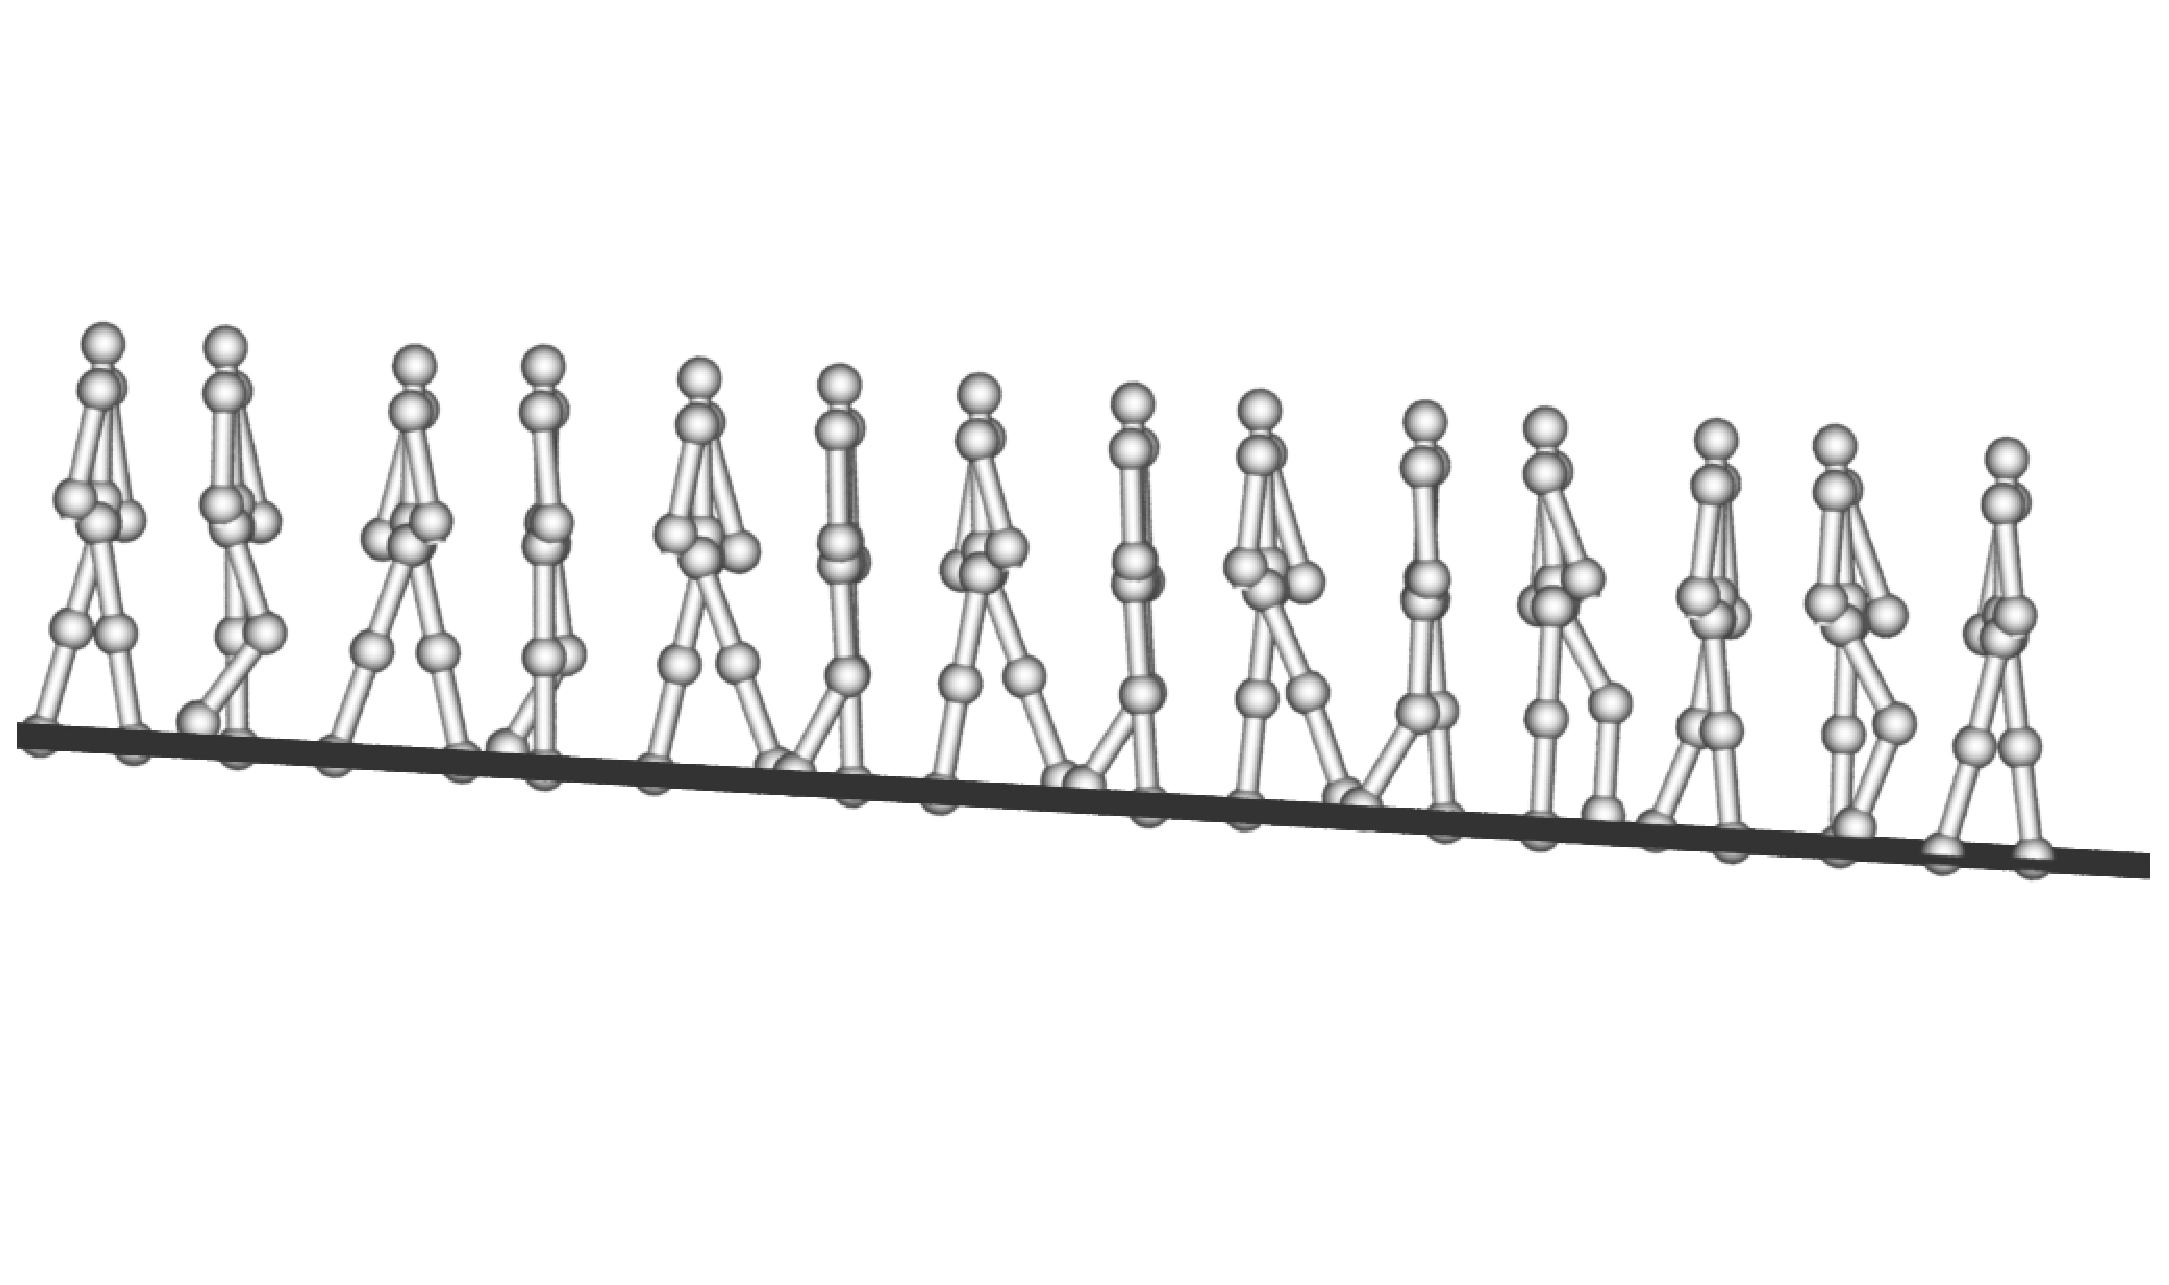
\includegraphics[width=0.7\textwidth]{PushGait}
    \caption{The Push Perturbated Gait}
    \label{fig:PushGait}
\end{center}
\end{figure}


\begin{figure}[!htbp]
  \begin{center}
      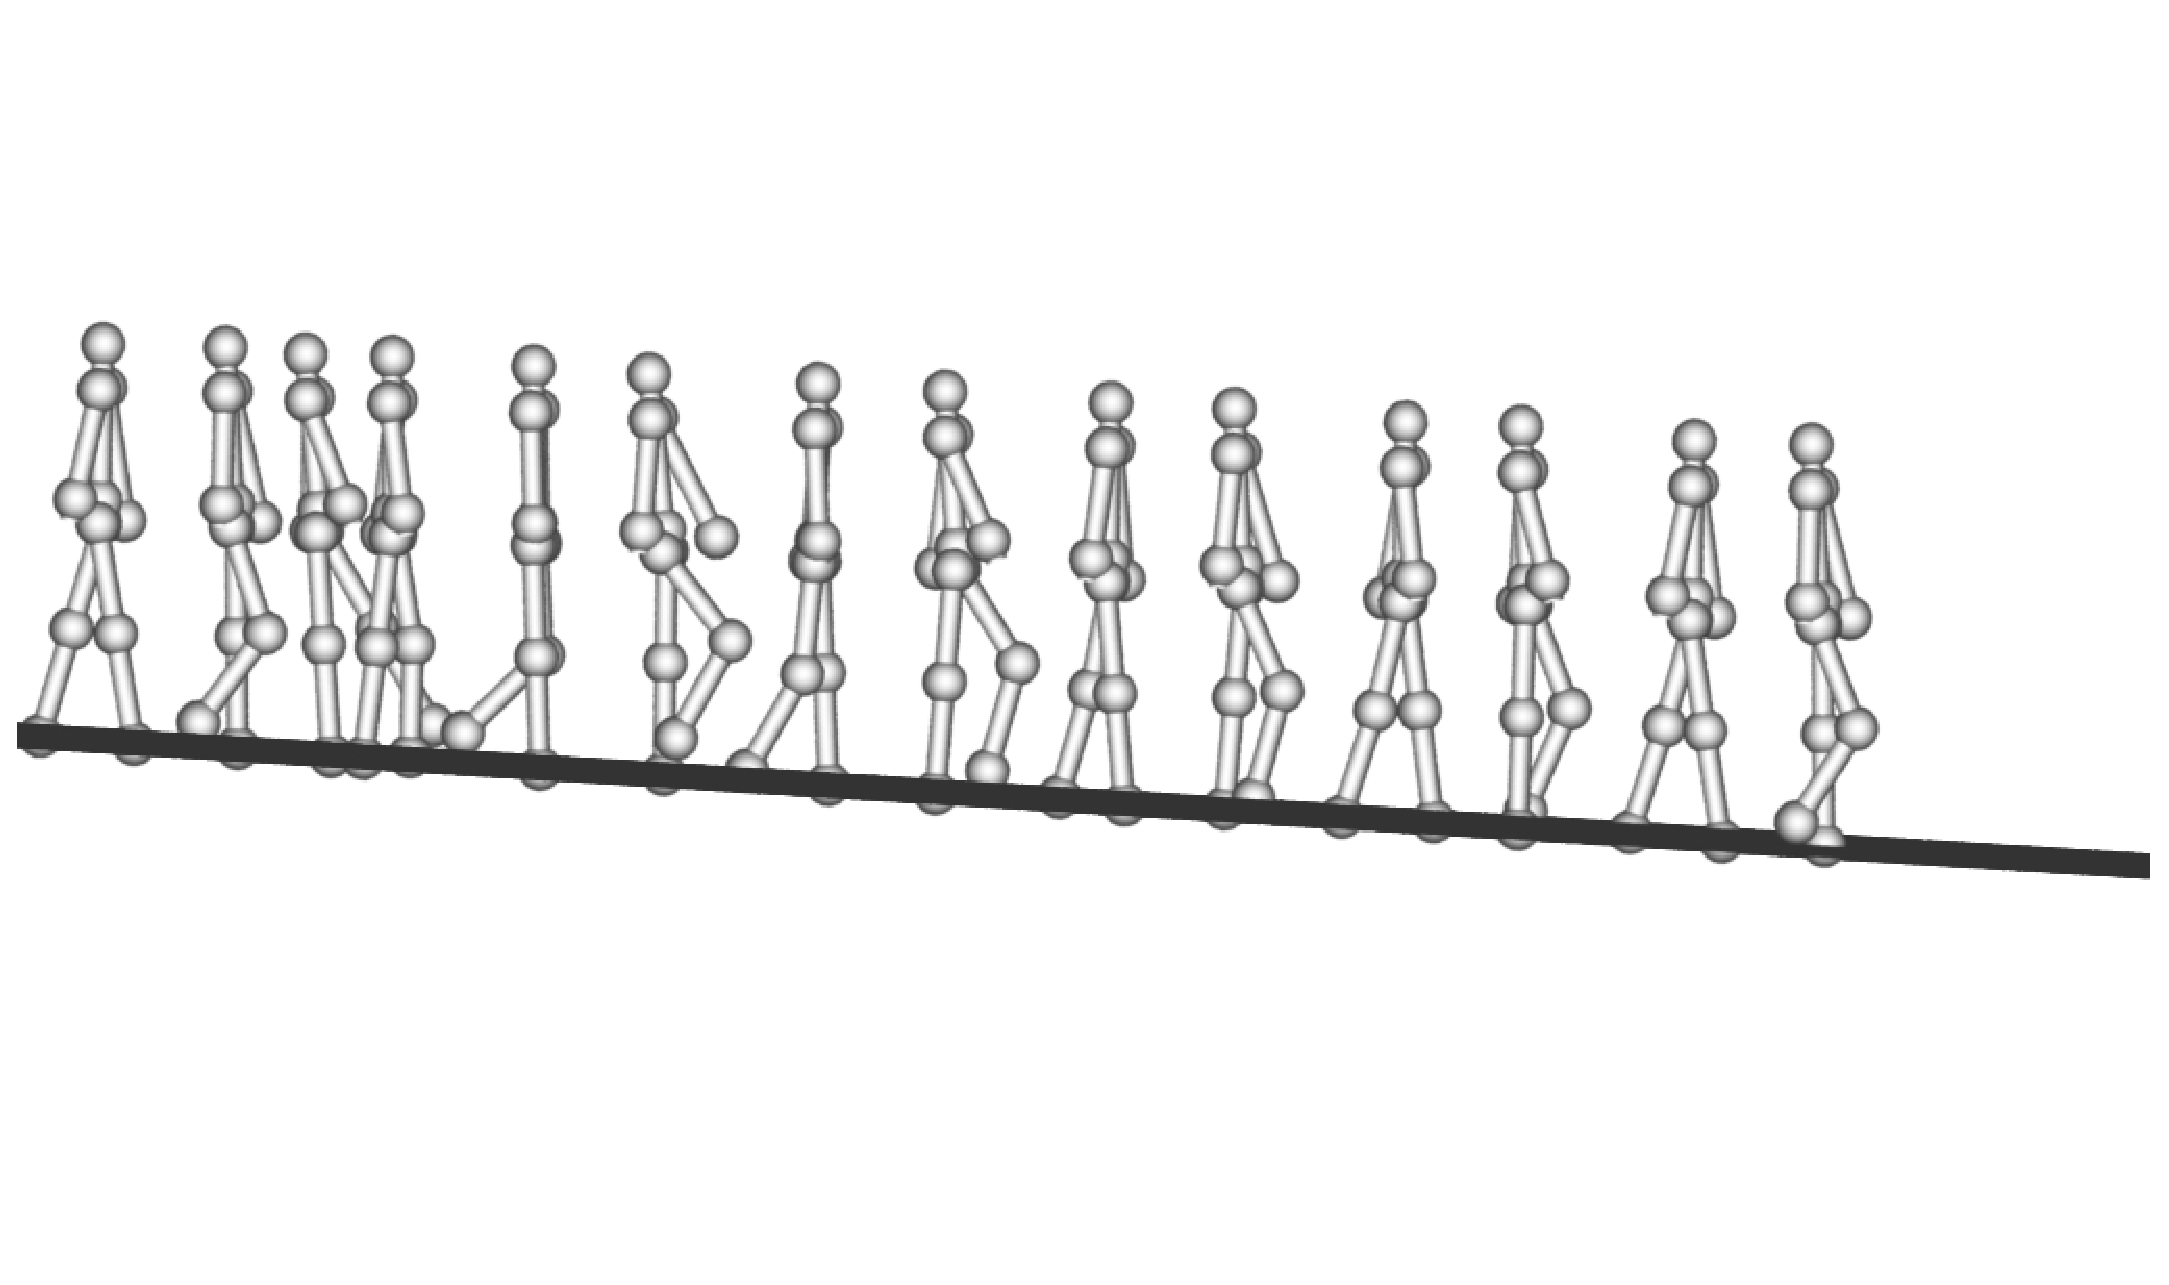
\includegraphics[width=0.7\textwidth]{PullGait}
    \caption{The Pull Perturbated Gait}
    \label{fig:PullGait}
\end{center}
\end{figure}

Figure~\ref{fig:PushGaitPlot} and Figure~\ref{fig:PullGaitPhasePlot} show the flow convergence of the limit cycle.
When the character is pushed, it takes a big walking cycle. 
However because of the entrainment, the walking cycle shrinks and trembles around the limit cycle. 
The pull effects make the character take a smaller step size, in the next several steps, the walker takes bigger and smaller step to adjust walking and finally returns to the normal walking gait.


\begin{figure}[!htbp]
  \begin{center}
      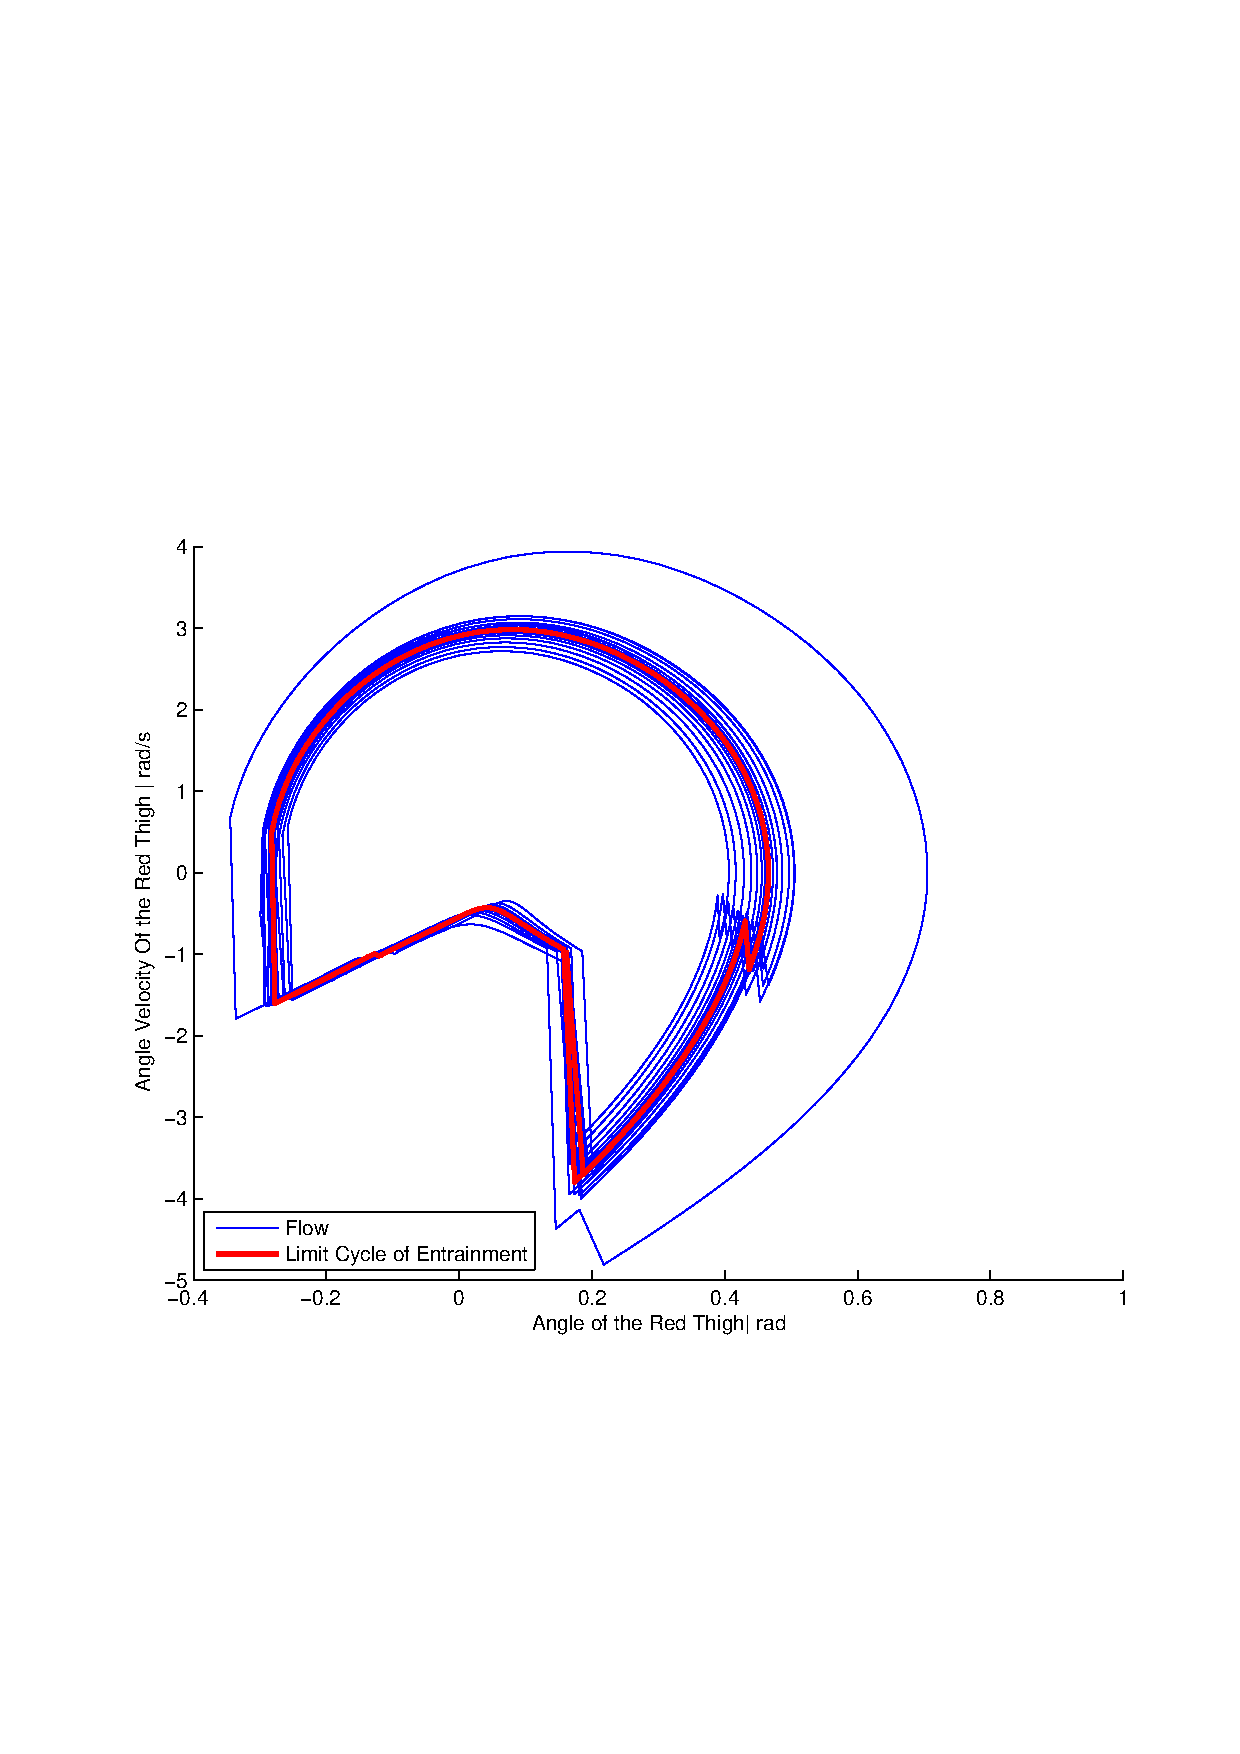
\includegraphics[width=0.7\textwidth]{PushWalkingPhasePlot}
    \caption{The Pushed Gait Phase Plot}
    \label{fig:PushGaitPlot}
\end{center}
\end{figure}


\begin{figure}[!htbp]
  \begin{center}
      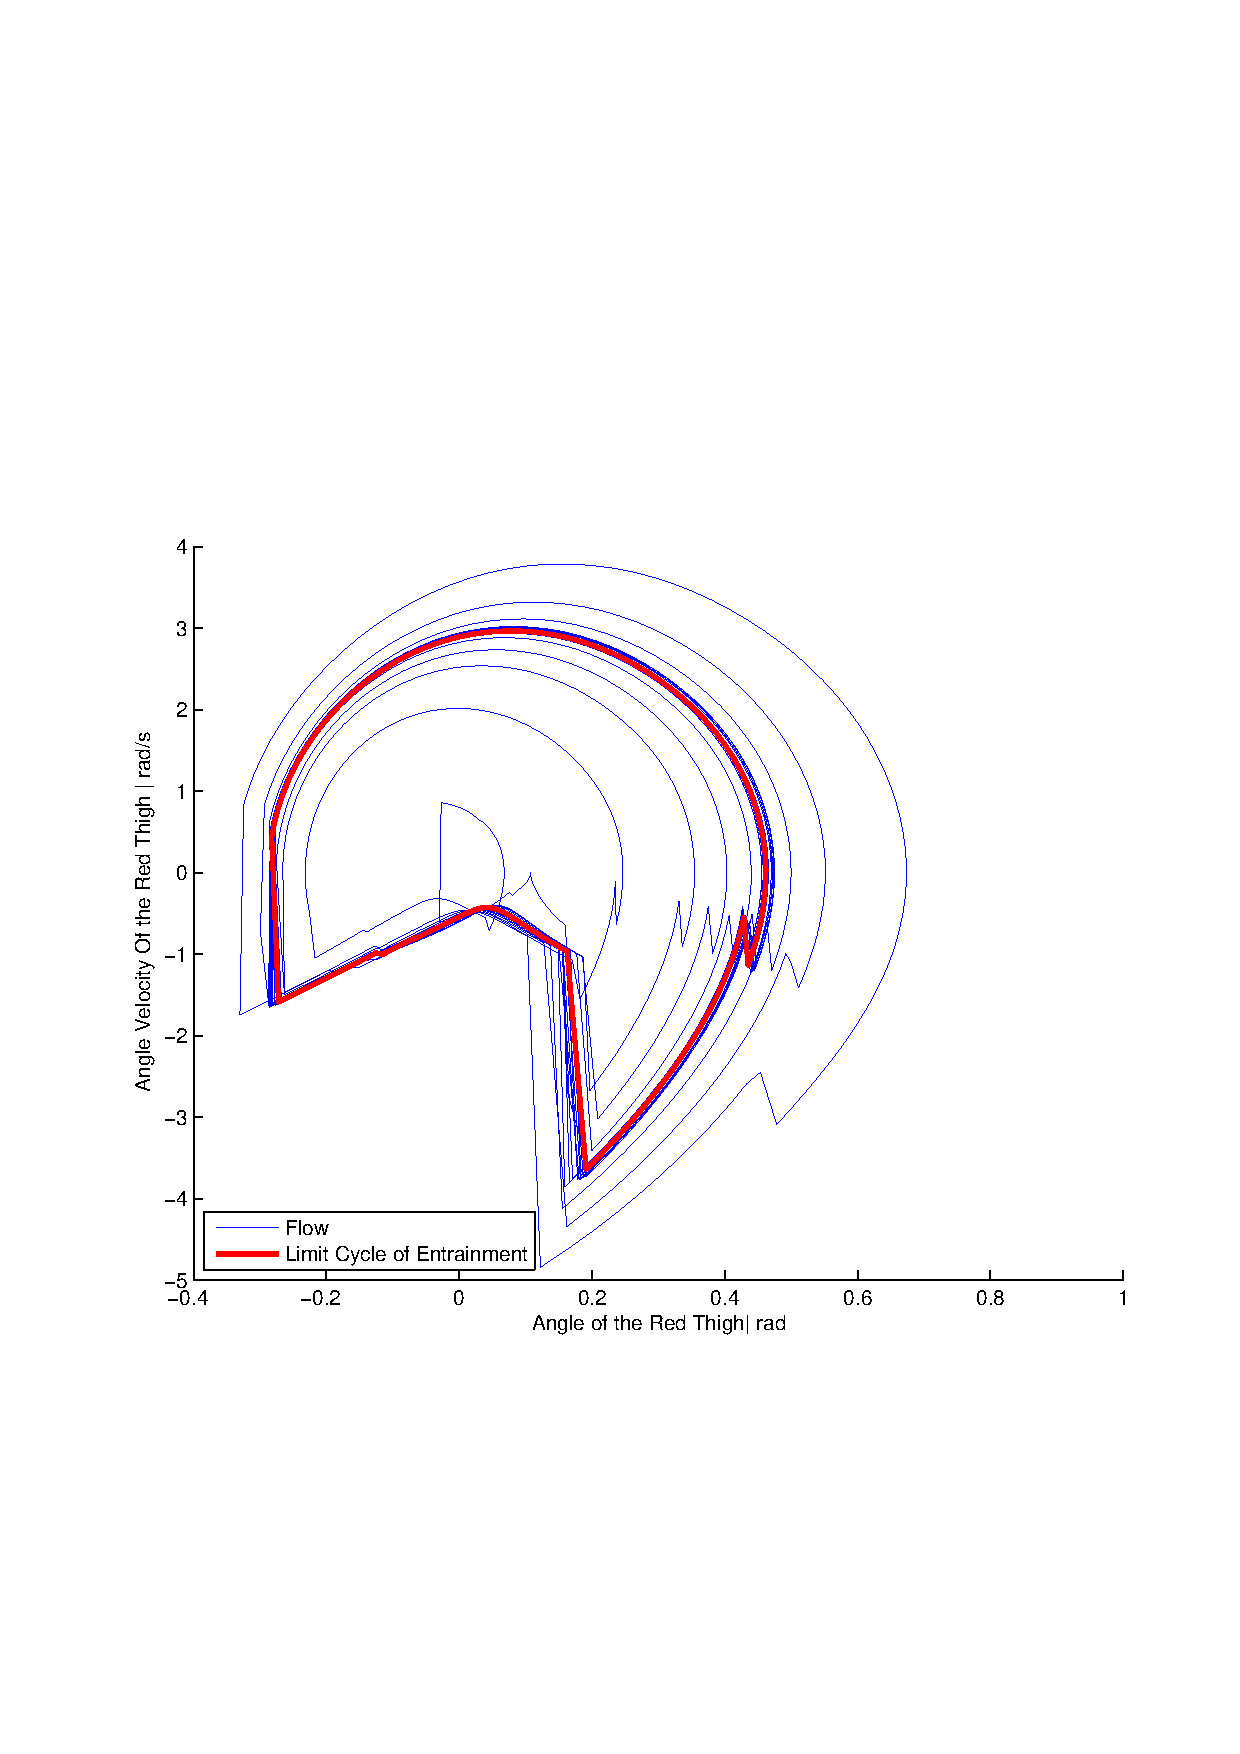
\includegraphics[width=0.7\textwidth]{PullWalkingPhasePlot}
    \caption{The Pulled Gait Phase Plot}
    \label{fig:PullGaitPhasePlot}
\end{center}
\end{figure}


The initial step size can also be changed, the walker will adjust it automatically.
Figure~\ref{fig:bigStepIni} and Figure~\ref{fig:smallStepini} show the gaits.
Figure~\ref{fig:bigstepiniGaitPlot} and Figure~\ref{fig:smallstepiniPhasePlot} show the phase plot.

\begin{figure}[!htbp]
  \begin{center}
      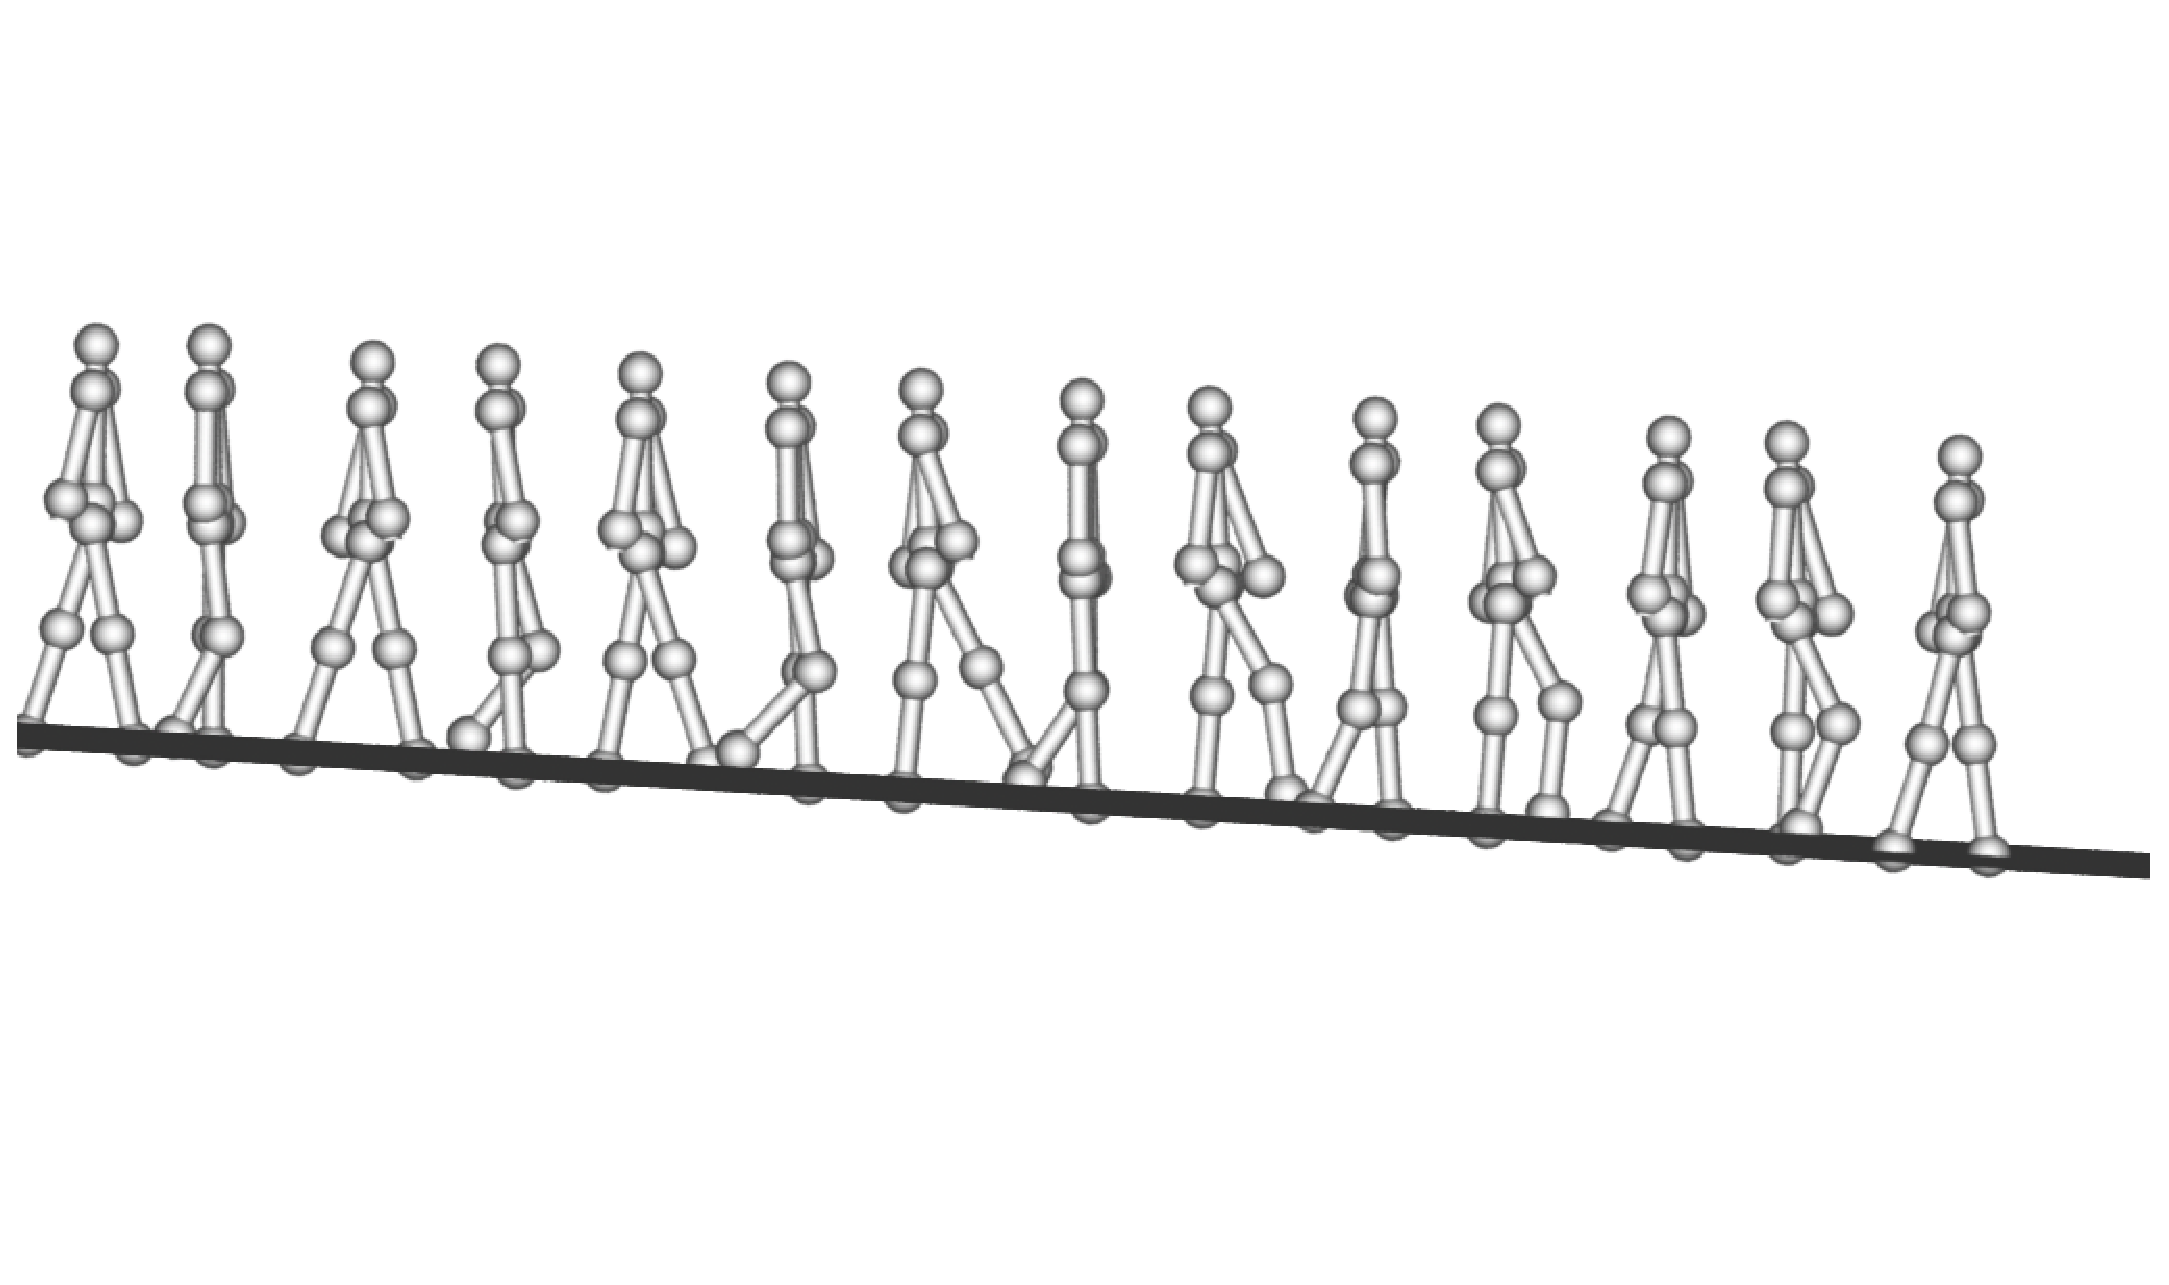
\includegraphics[width=0.7\textwidth]{BigStep}
    \caption{Big Initial Step Size}
    \label{fig:bigStepIni}
\end{center}
\end{figure}


\begin{figure}[!htbp]
  \begin{center}
      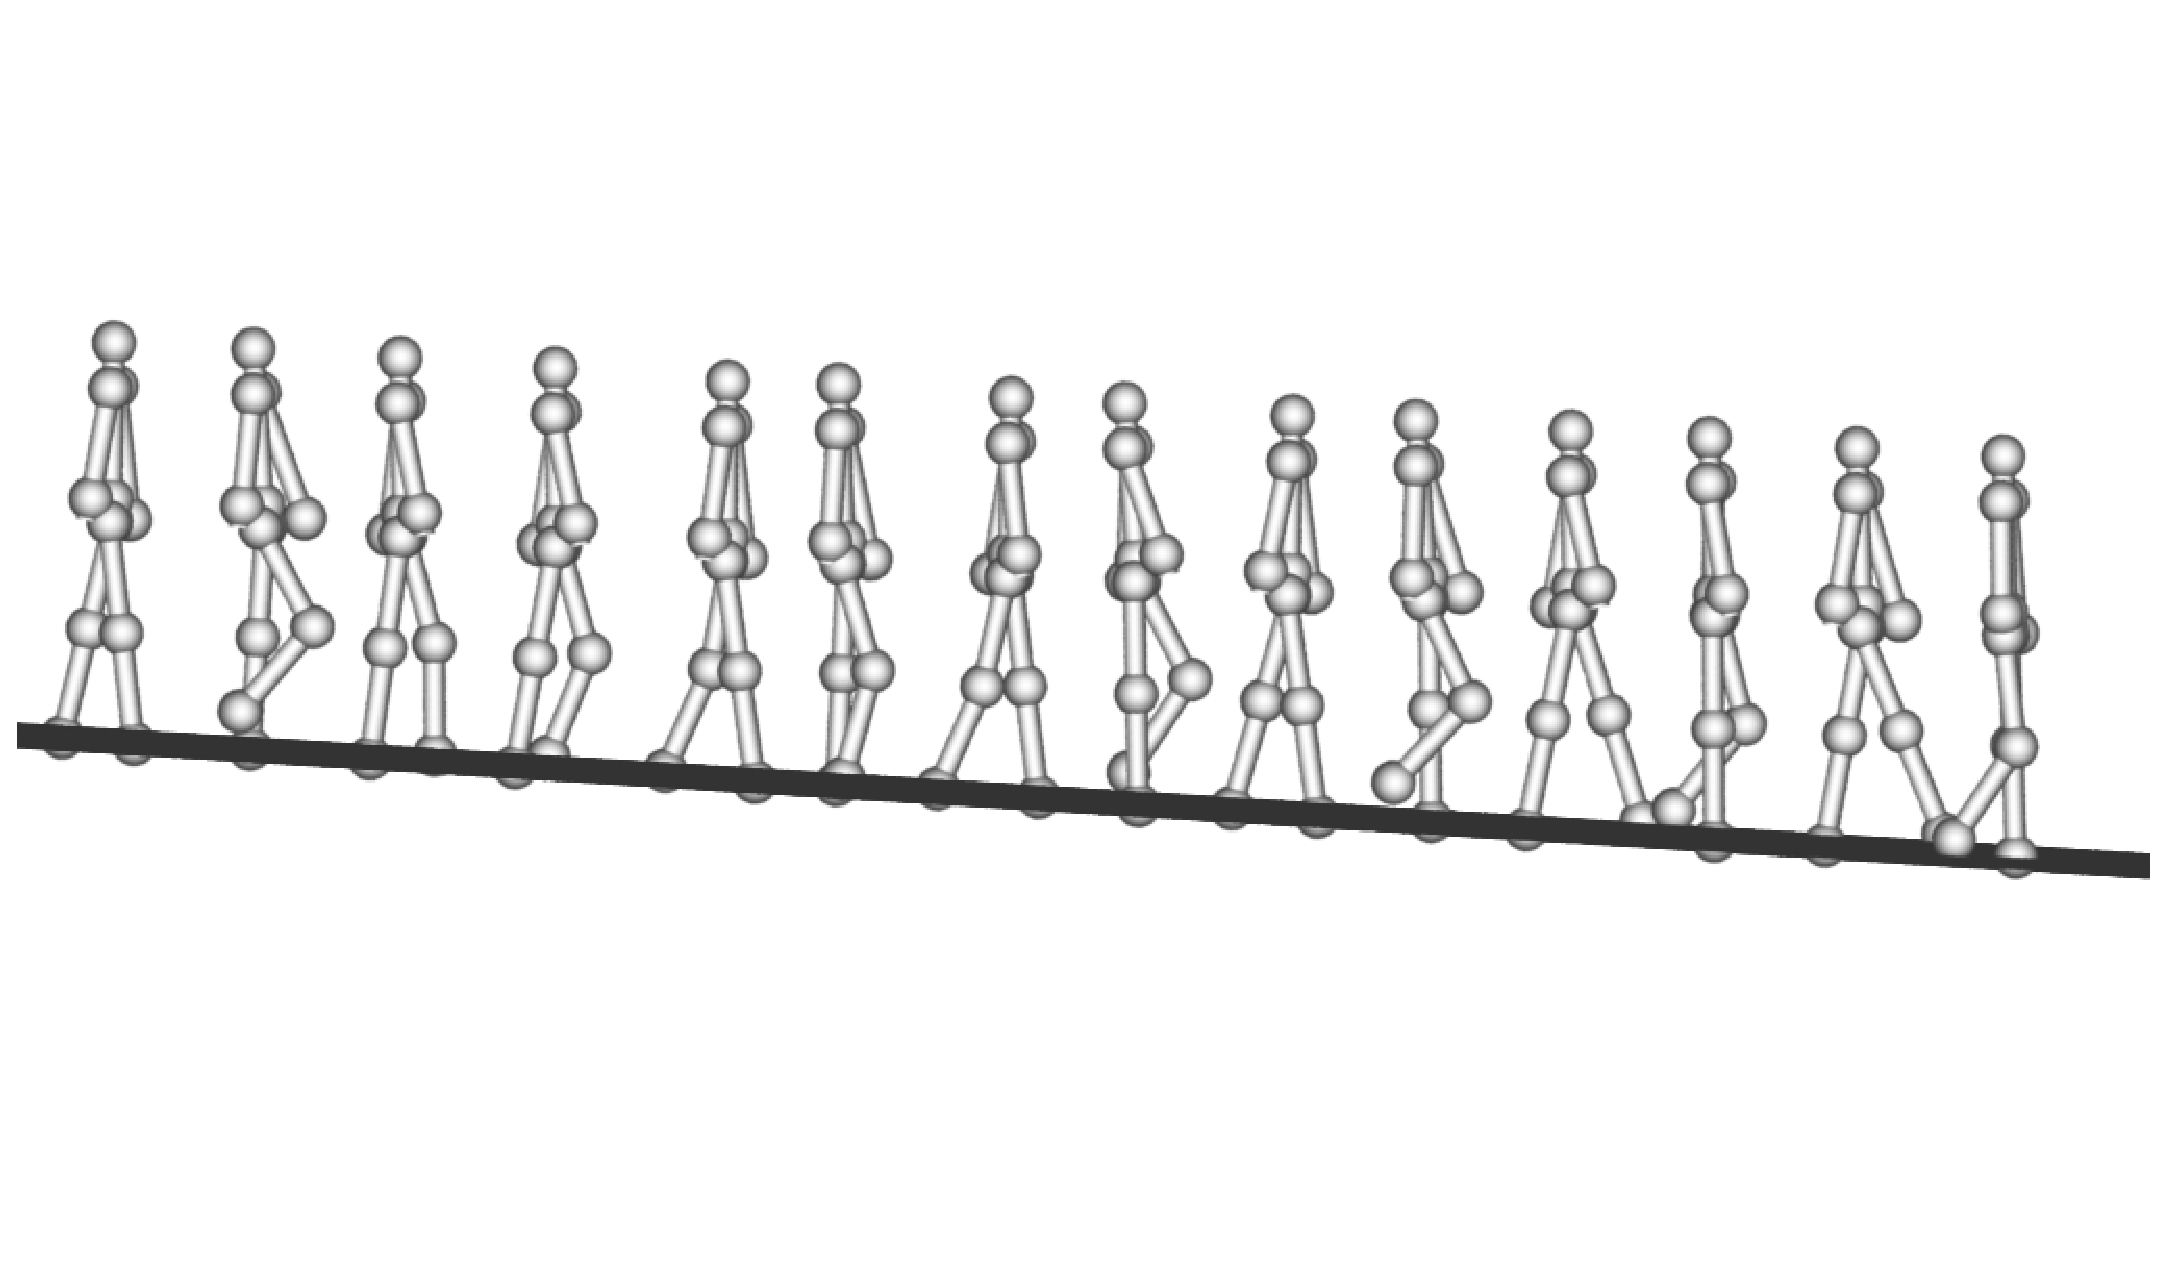
\includegraphics[width=0.7\textwidth]{smallStep}
    \caption{Small Initial Step Size}
    \label{fig:smallStepini}
\end{center}
\end{figure}


\begin{figure}[!htbp]
  \begin{center}
      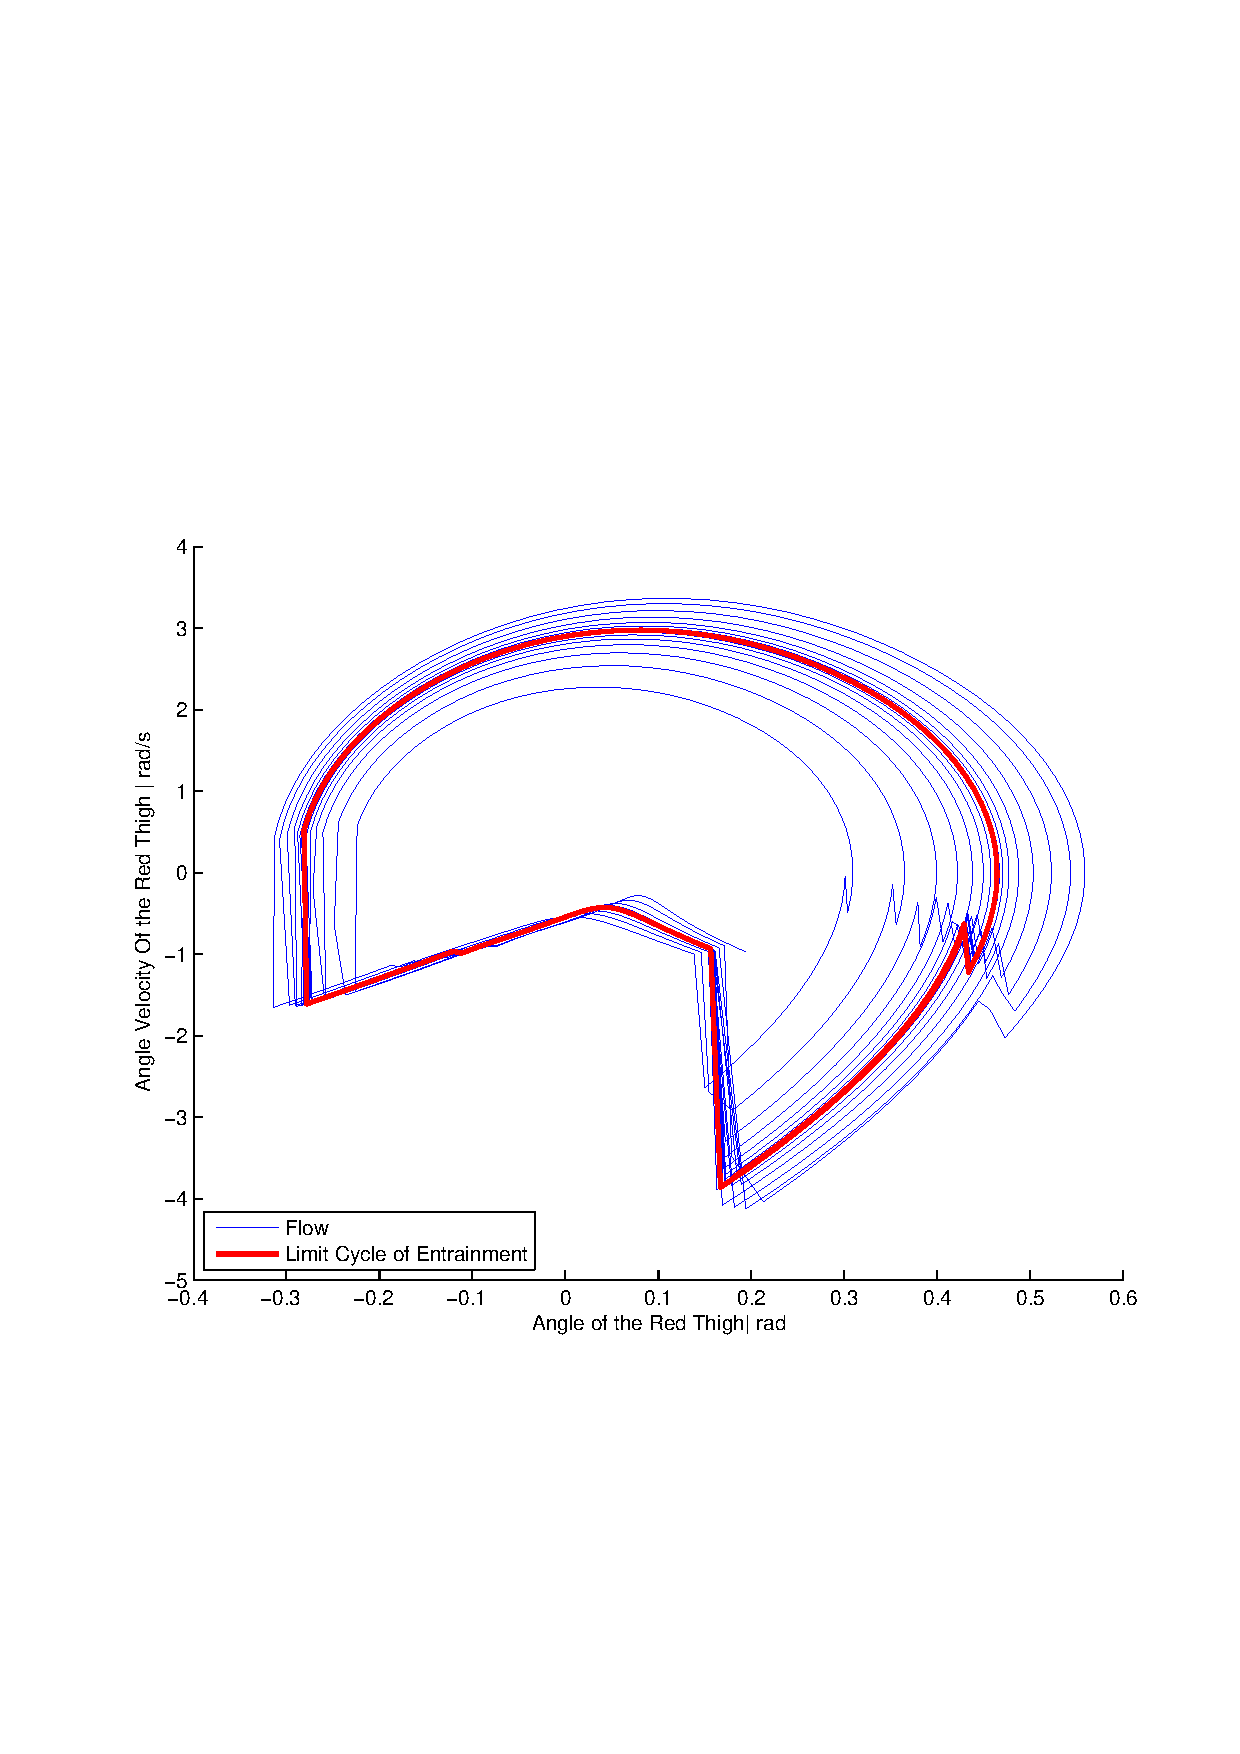
\includegraphics[width=0.7\textwidth]{BigStepPhasePlot}
    \caption{Big Initial Step Initial Phase Plot}
    \label{fig:bigstepiniGaitPlot}
\end{center}
\end{figure}


\begin{figure}[!htbp]
  \begin{center}
      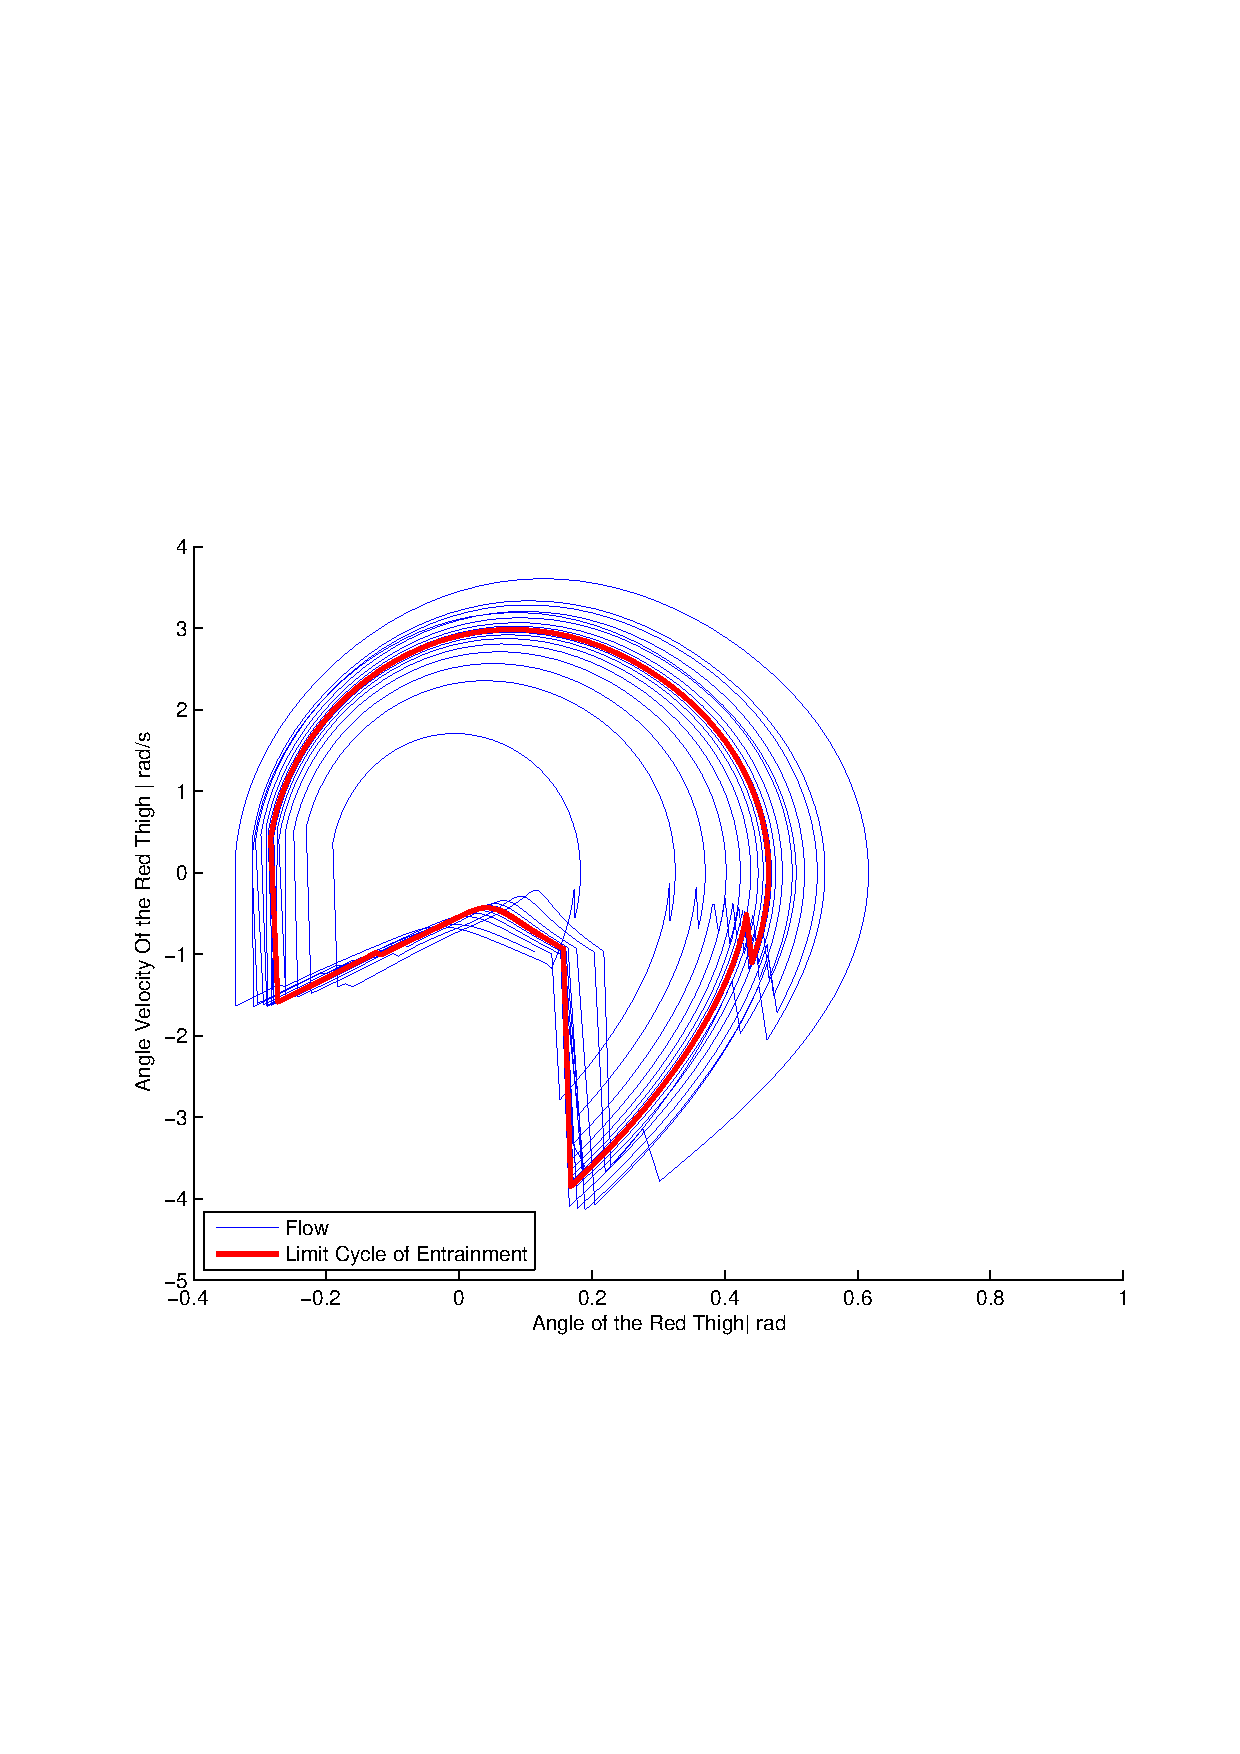
\includegraphics[width=0.7\textwidth]{SmallStepPhasePlot}
    \caption{The Small Initial Step Gait Phase Plot}
    \label{fig:smallstepiniPhasePlot}
\end{center}
\end{figure}

The entrainment of \cpg greatly enlarge the basin of attraction, when the parameters of \cpg is fixed, even start with very different position, the character will return to normal walk.





\subsection{Walking Re targeting}
Transferring the gait of one character to another is an challenging job.
\moit theory provides a method for physics based motion re-targeting.
\cpg will maintain the topology of the dynamics, when the dynamic parameters are changed, the analogous system will result in a varied motion.

The passive walker has many parameters, like mass and leg length.
Different parameters will result in a different dynamics system.
But all these dynamic systems  share the same topology and generate different limit cycle and gaits.
Some meaningful gaits are shown in this section.

If all the parameters are scaled in uniform, the gait will remain the same, only the velocity will be changed.
To demonstrate different gaits, the ratio or relative parameters are modified. 
The total mass and total leg length of all examples are kept the same.



\subsubsection*{Mass Distribution Ratio}
When the total mass is kept,
Mass Distribution Ratio is defined as the hip mass over leg mass. 
\[
\alpha_m=\frac{m_h}{m_s}
\]
where $m_h$ is the mass of the hip and $m_t$ is mass of the thigh.
The mass ratios of shank and thigh are kept.

Different $\alpha_m$ will result in different gaits, bigger $\alpha_m$ result gait to that burdened.
Different limit cycles are shown in Figure ~\ref{fig:differentmh}.
\begin{figure}[!htbp]
  \begin{center}
     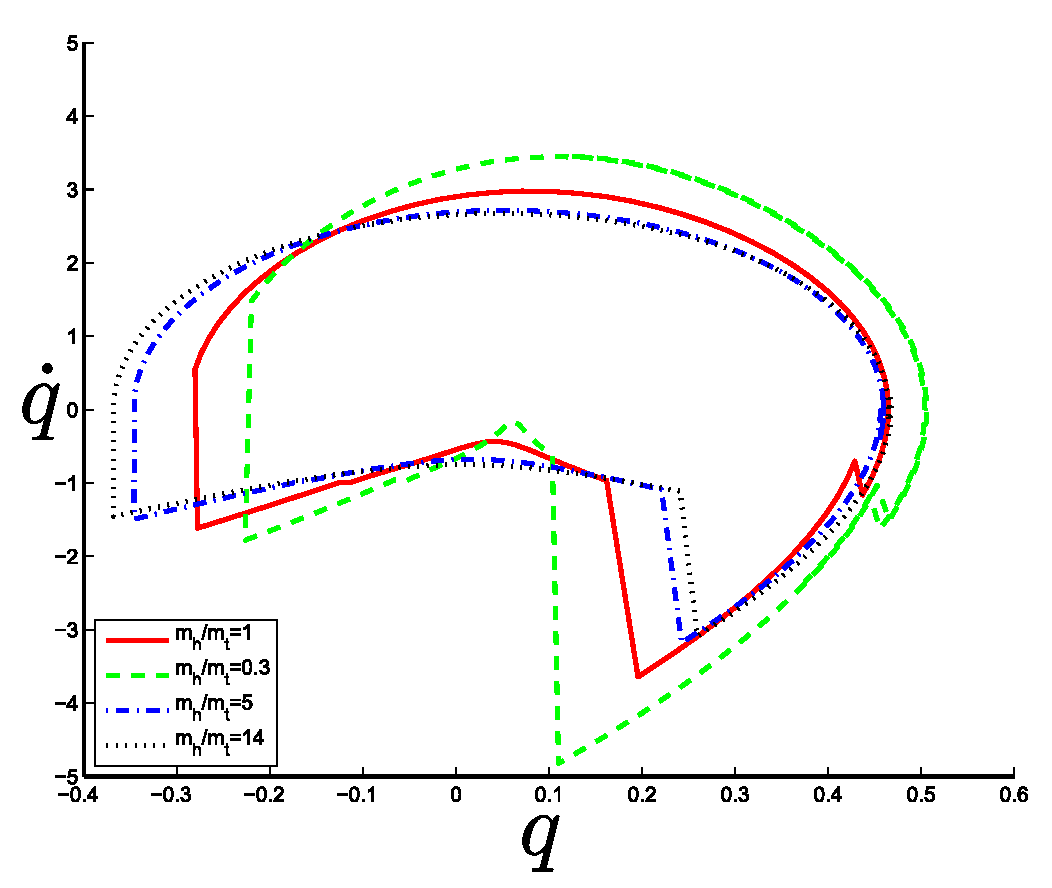
\includegraphics[width=0.7\textwidth]{MassDistributionEffectsOnLimitCircle}
    \caption{Different Gait Resulting from the Different Mass Ratio}
    \label{fig:differentmh}
\end{center}
\end{figure}

For bigger $\alpha_m$, the walker will walk with bigger step but a slow speed($\qd$ is lower).
Also the character tends to fall backward.
For smaller $\alpha_m$, character will walk quickly($\qd$ is bigger) and it tends to lean forward.
This may imply about the upper body motion.
Usually, when we carry something heavier, we  tend to bend upper body forward.

Different gaits are shown in Figure~\ref{fig:massh1},Figure~\ref{fig:massh2} and Figure~\ref{fig:massh3}
\begin{figure}[!htbp]
  \begin{center}
      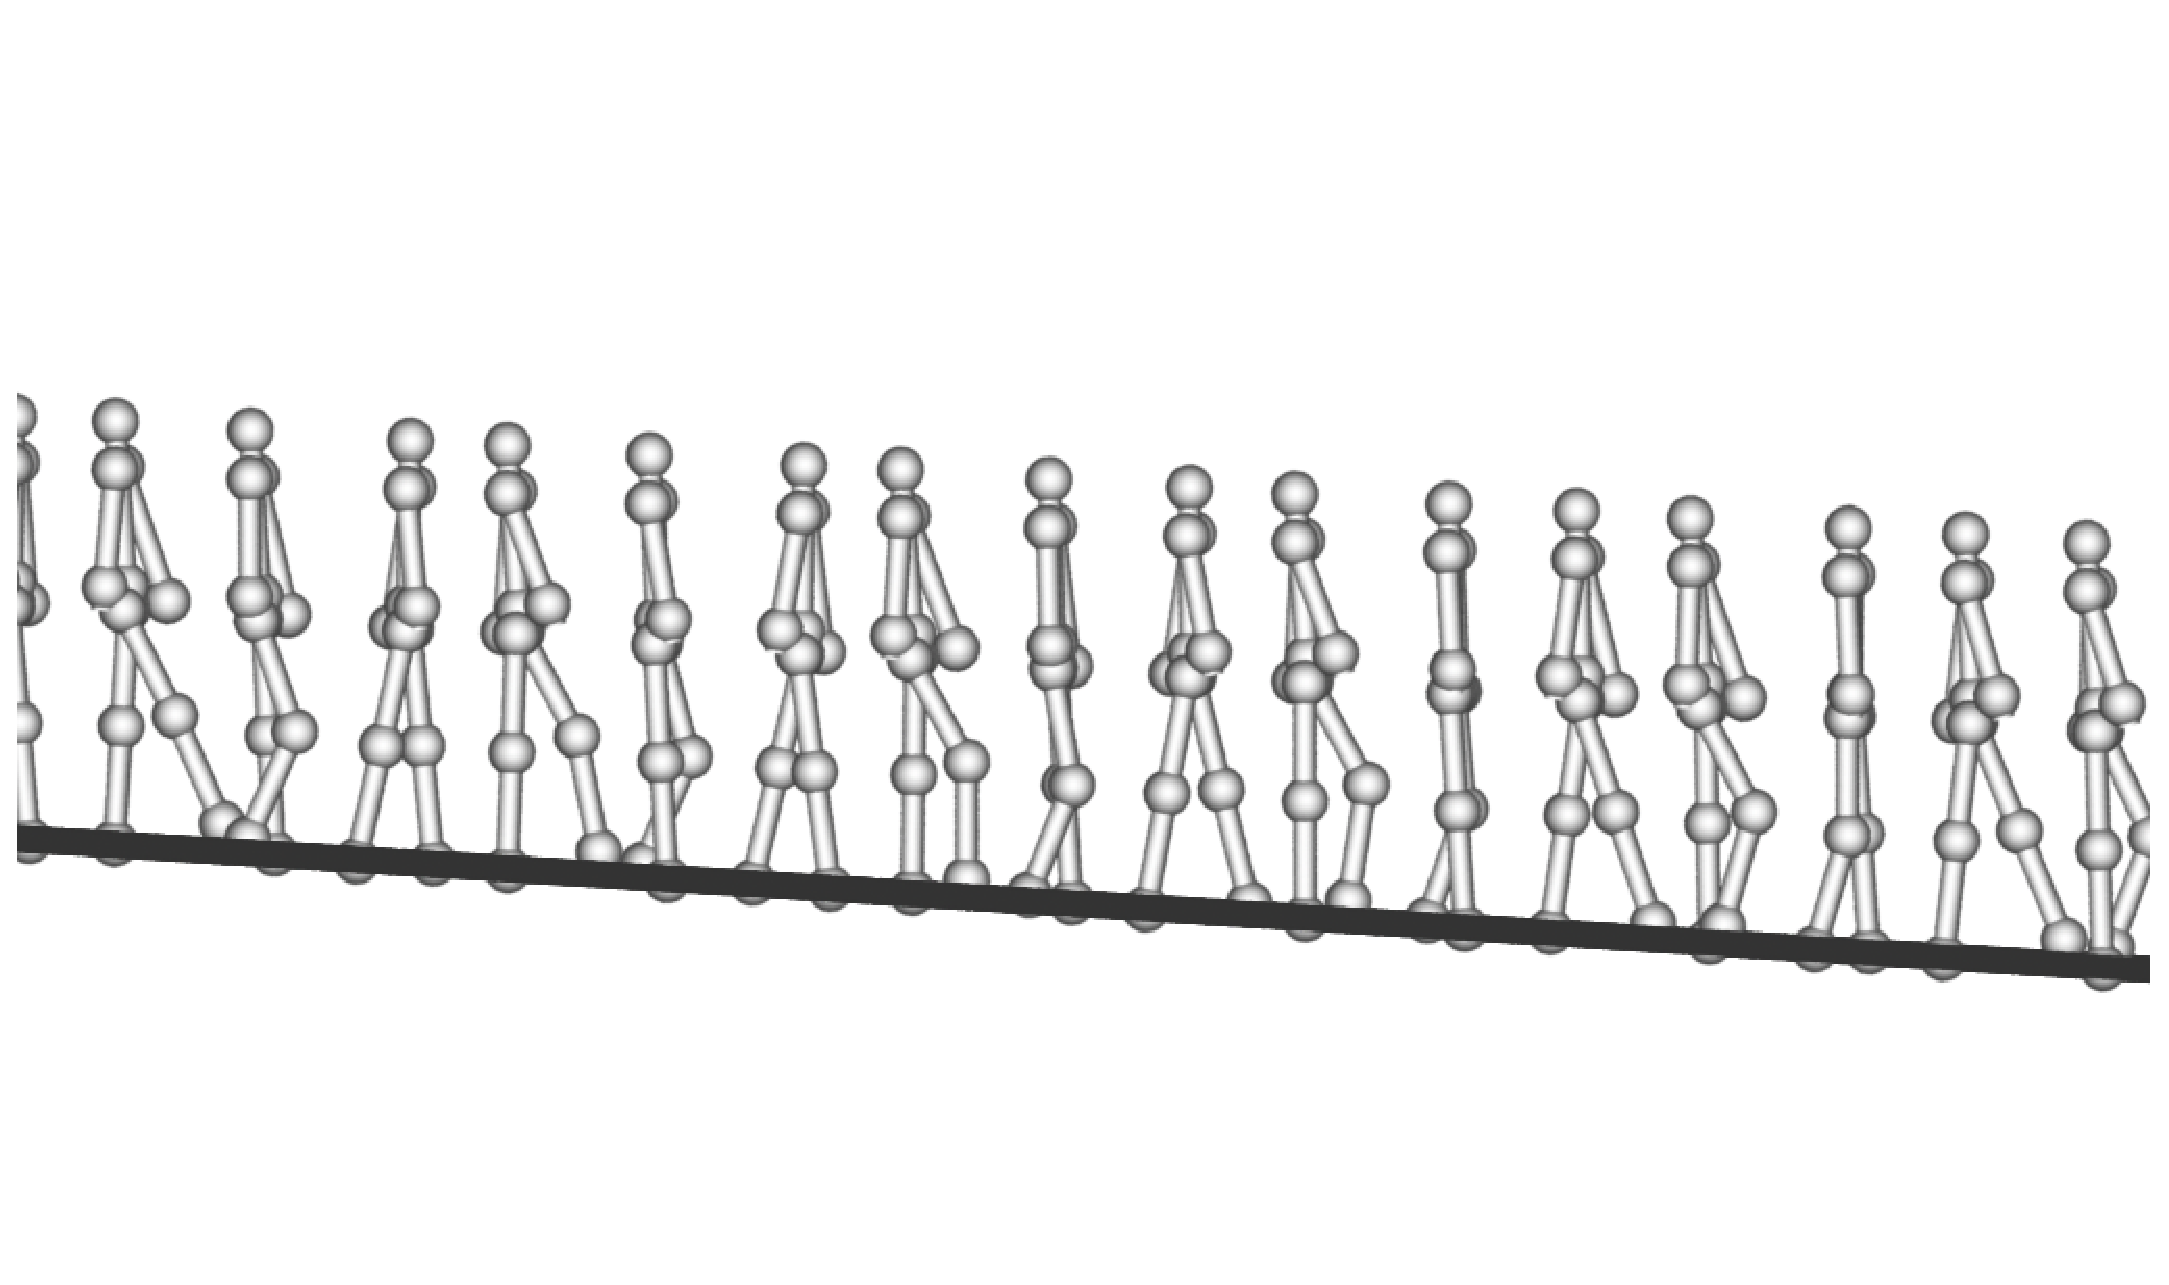
\includegraphics[width=0.7\textwidth]{mhms3}
    \caption{gait with $\alpha_m=0.3$}
    \label{fig:massh1}
\end{center}
\end{figure}

\begin{figure}[!htbp]
  \begin{center}
      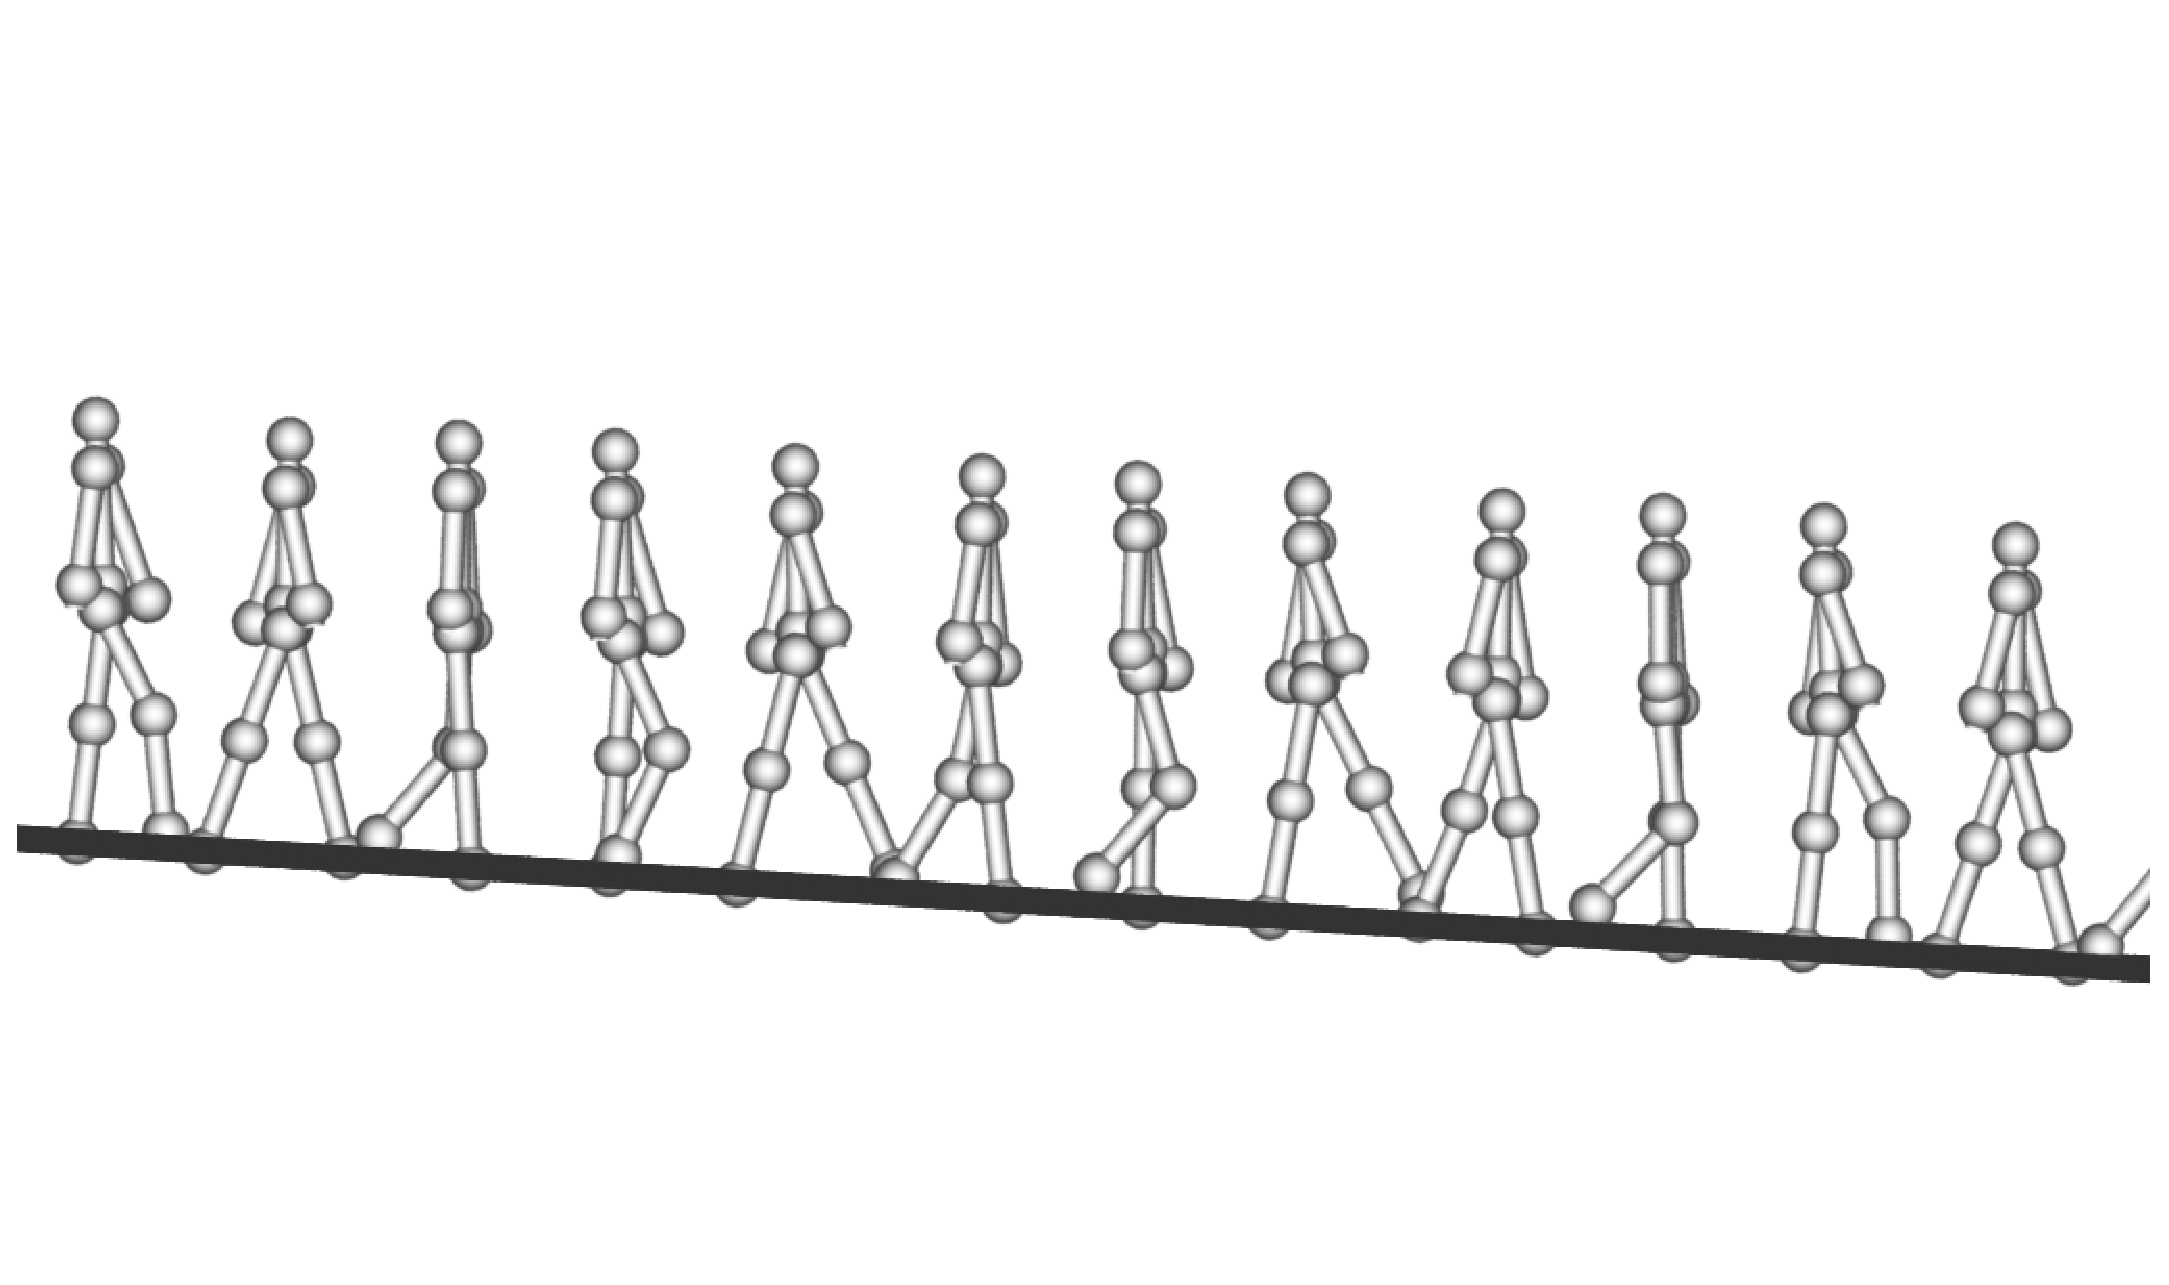
\includegraphics[width=0.7\textwidth]{mhms50}
    \caption{Gait of $\alpha_m=5$}
    \label{fig:massh2}
\end{center}
\end{figure}

\begin{figure}[!htbp]
  \begin{center}
      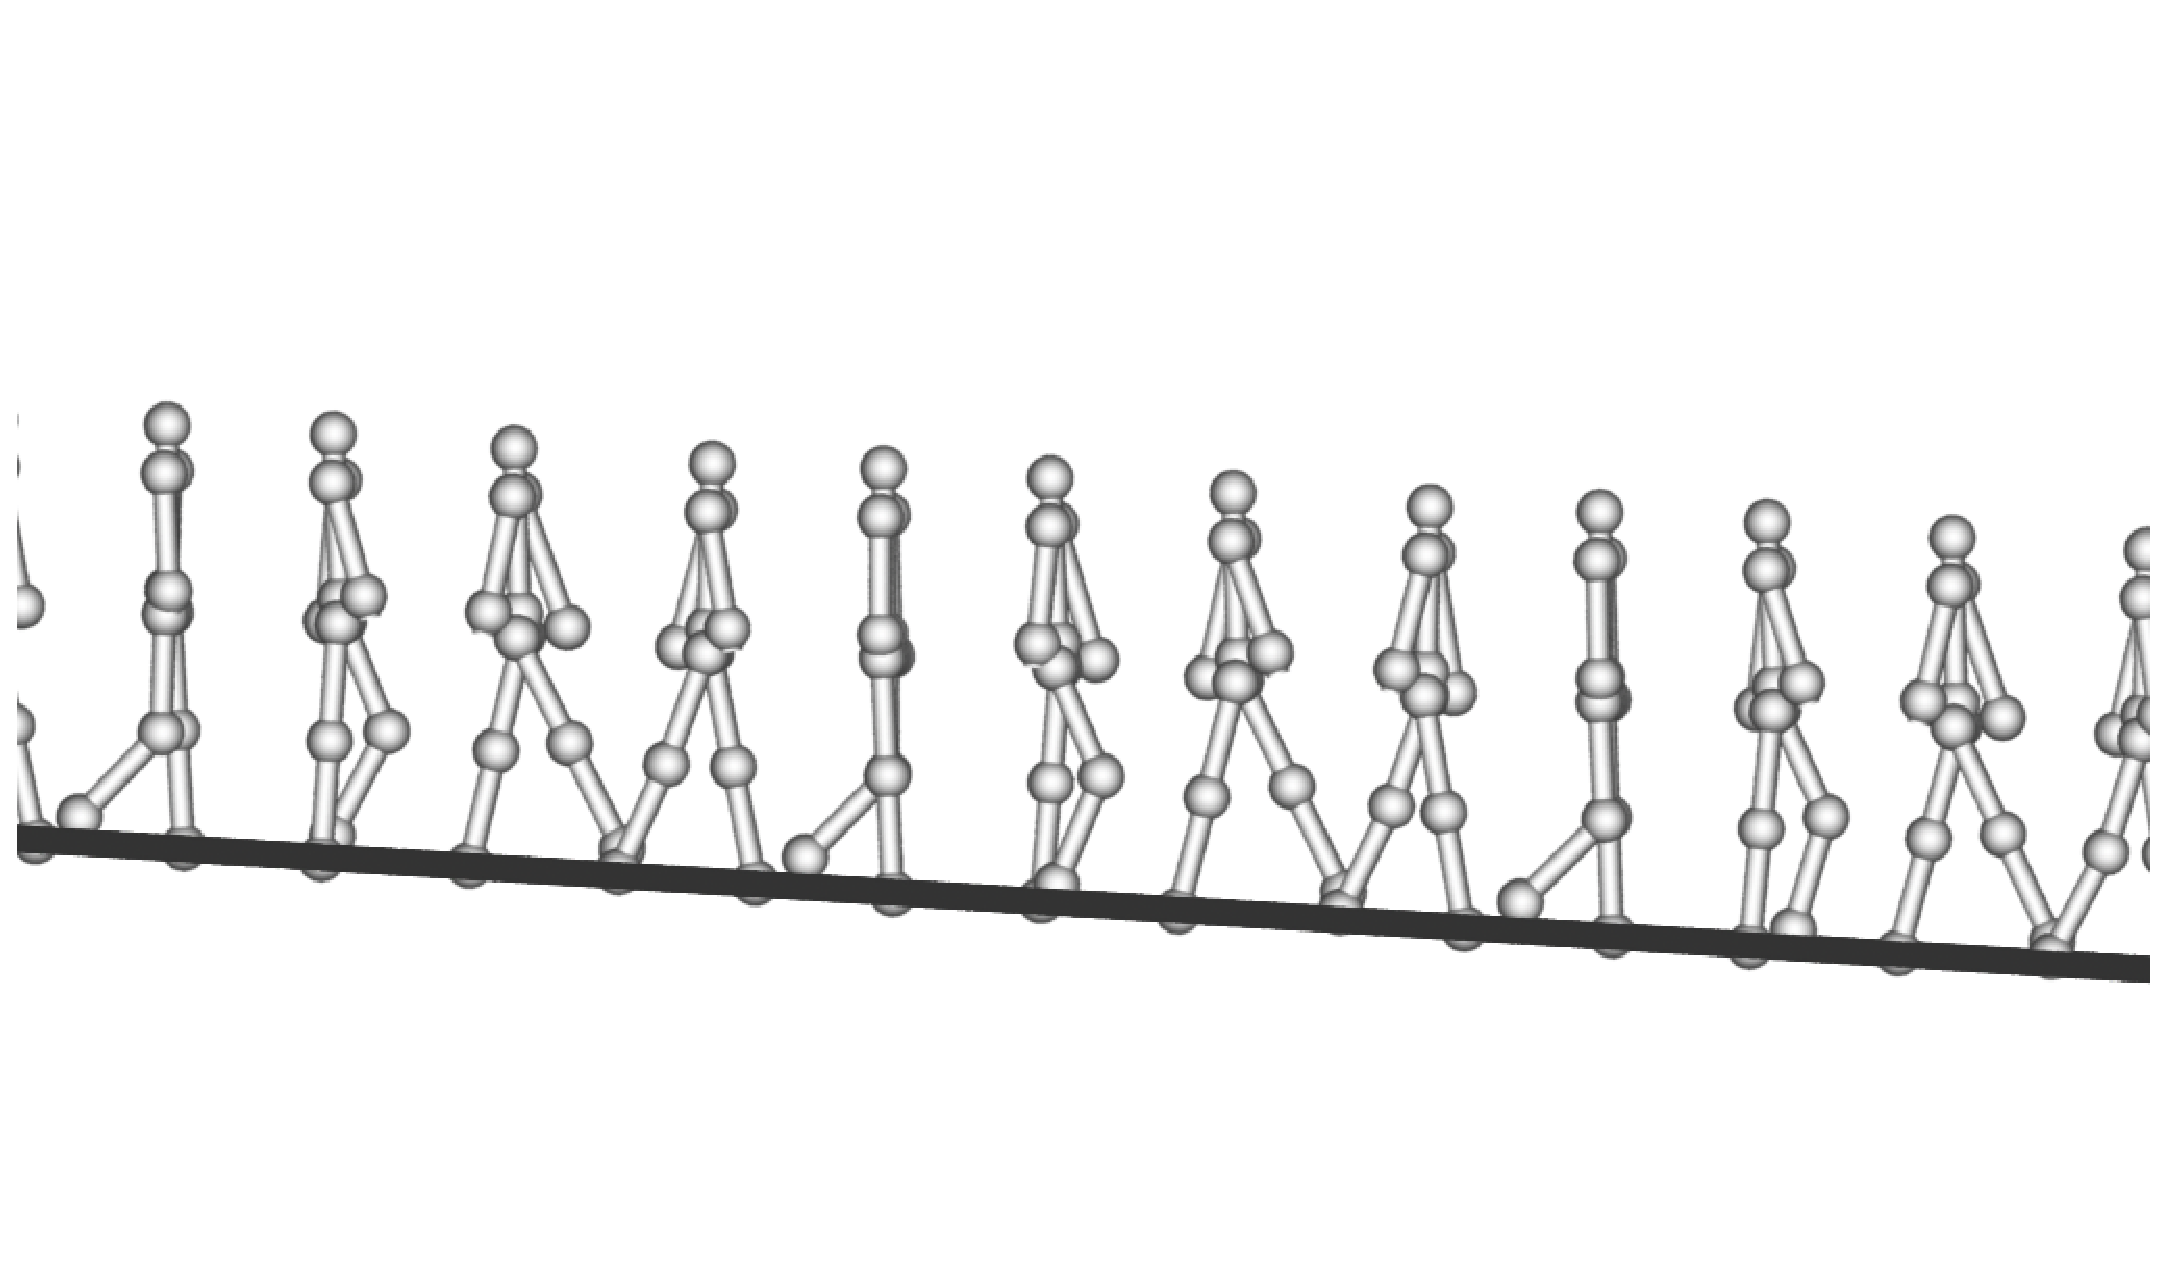
\includegraphics[width=0.7\textwidth]{mhms140}
    \caption{Gait of $\alpha_m=14$}
    \label{fig:massh3}
\end{center}
\end{figure}



\subsubsection*{Leg Length Distribution Ratio}
The leg length is kept unchanged, but we alter the the ration parameter $\alpha_l=\frac{l_t}{l_s}$.
By changing $\alpha_l$ motion for different characters are generated.
This demonstrated the motion re-targeting results.


\begin{figure}[!htbp]
  \begin{center}
      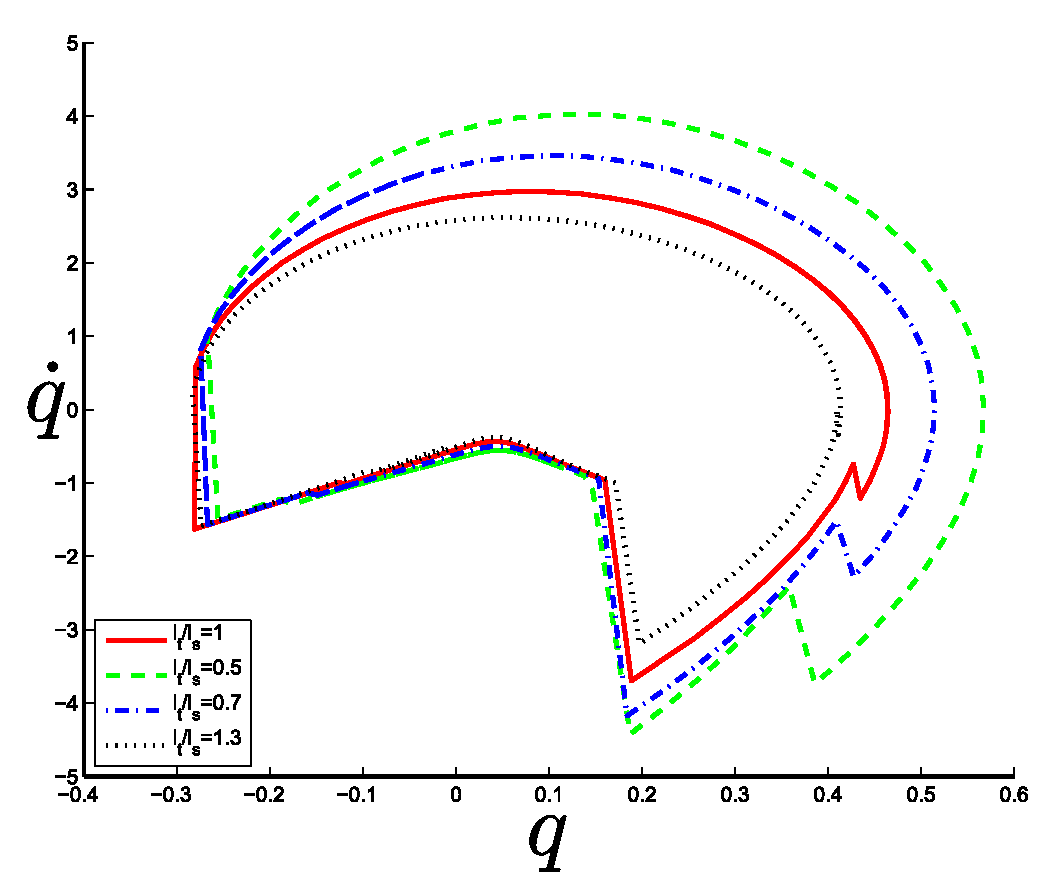
\includegraphics[width=0.7\textwidth]{LegLengthDistributionEffectsOnLimitCircle}
    \caption{Different Gait Resulting from the Different Mass Ratio}
    \label{fig:differentlr}
\end{center}
\end{figure}

The limit cycle in Figure~\ref{fig:differentlr} implies something important about leg length in walking.
Basically, the support leg motion is almost the same, while different leg length rations will result in different sway angle.
The step size is kept.
The longer the shank, thigh has to sway quickly and with bigger amplitude.
There are also bigger impulses during the strike phase. 
For both the knee and heel strike, larger impulse is generated.
This result may show the effects of high heel shoes for walking.

Figure~\ref{fig:lr1},Figure~\ref{fig:lr2},Figure~\ref{fig:lr3} show the different gaits.
\begin{figure}[!htbp]
  \begin{center}
      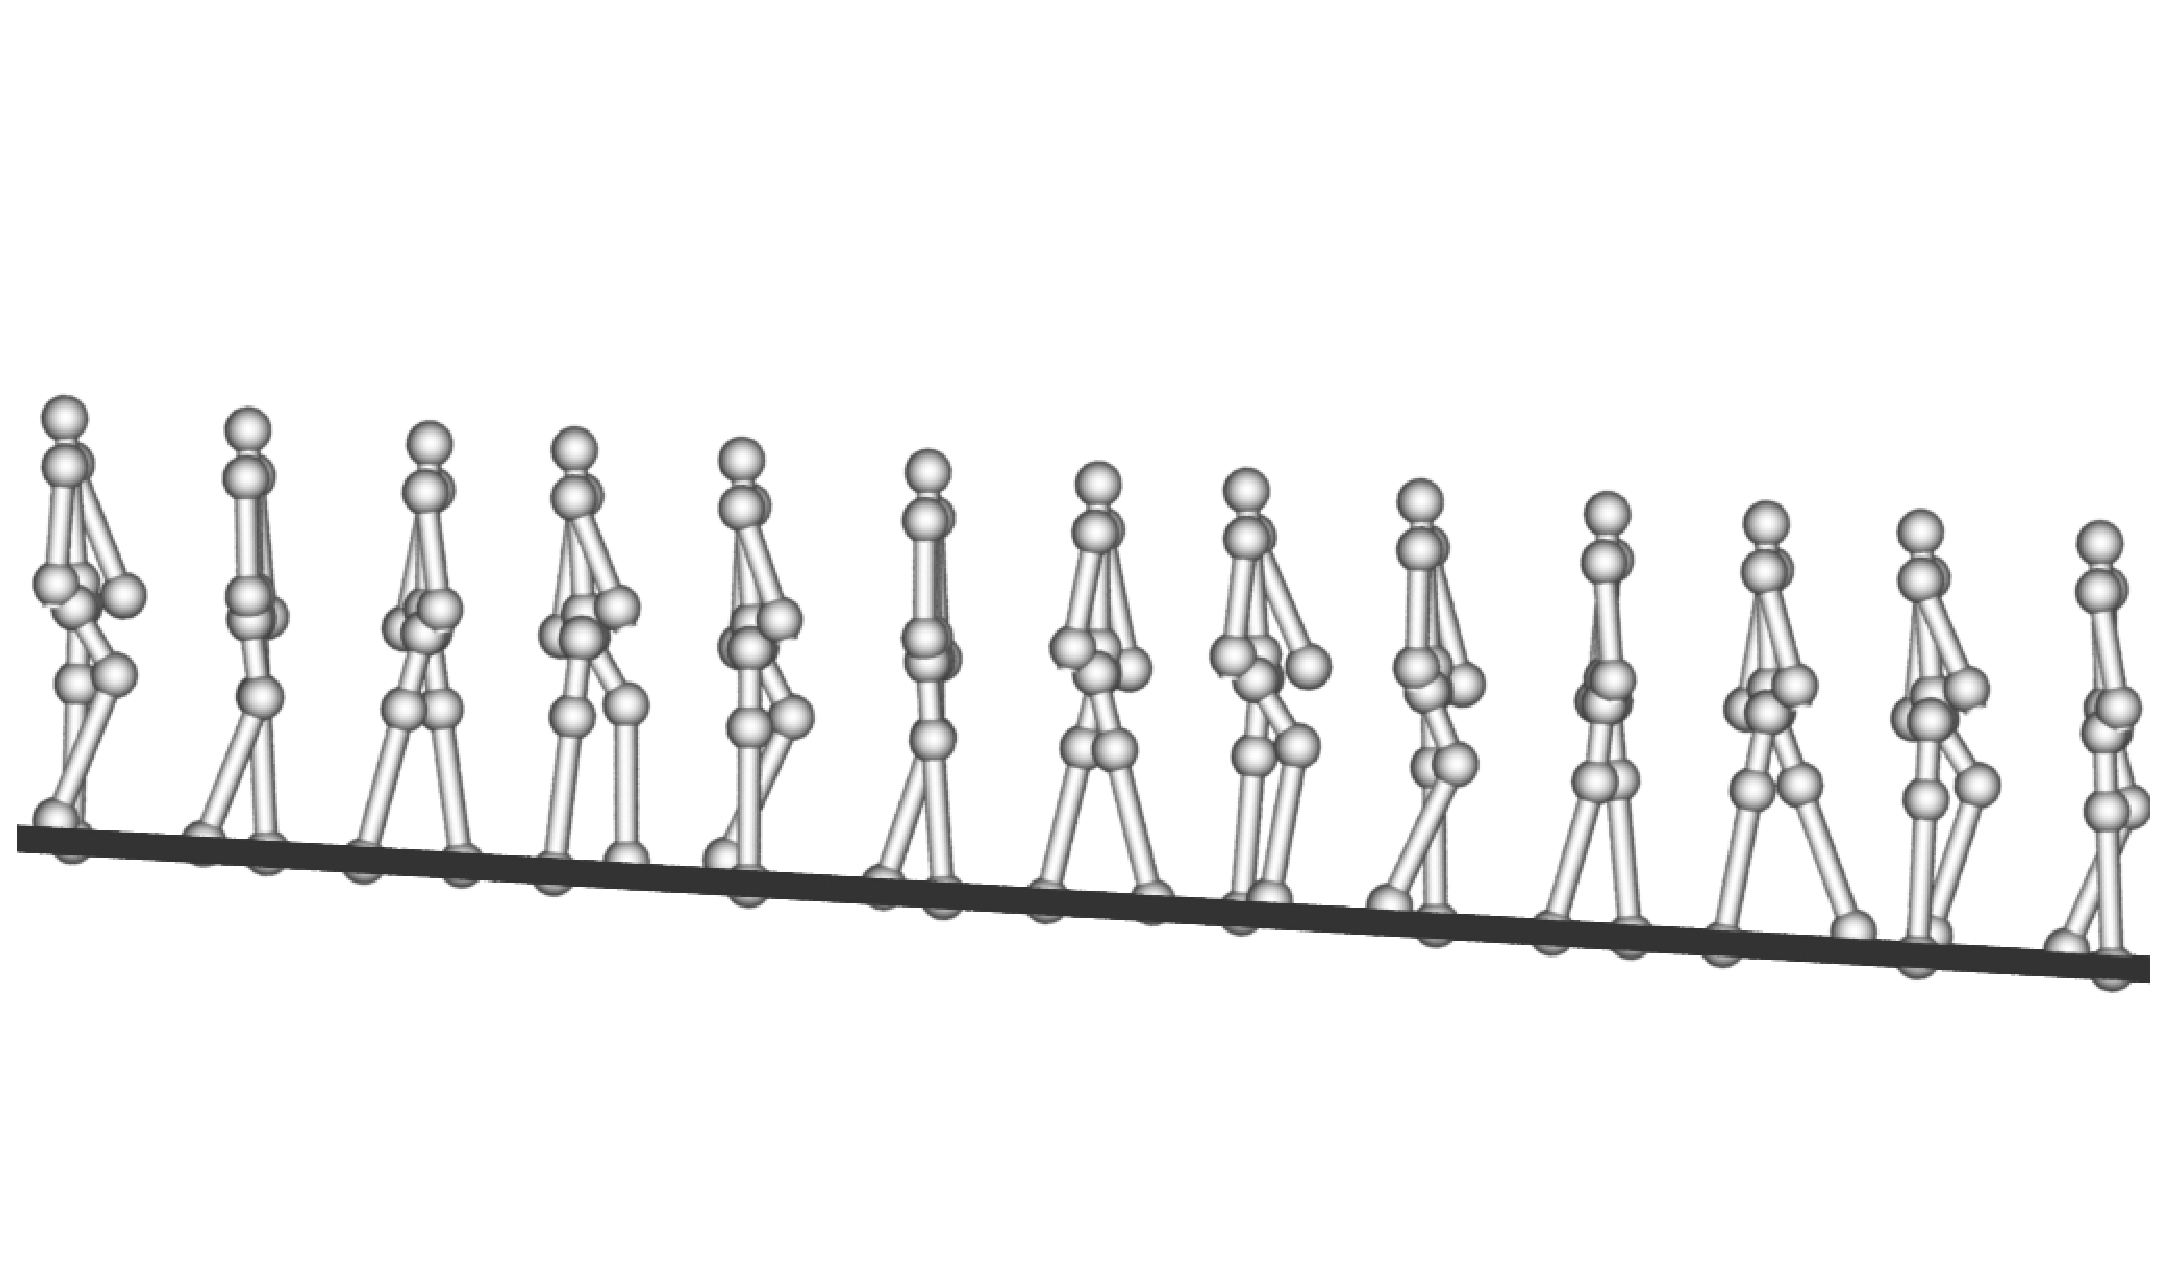
\includegraphics[width=0.7\textwidth]{LTLS5}
    \caption{gait of $\alpha_l=0.5$}
    \label{fig:lr1}
\end{center}
\end{figure}

\begin{figure}[!htbp]
  \begin{center}
      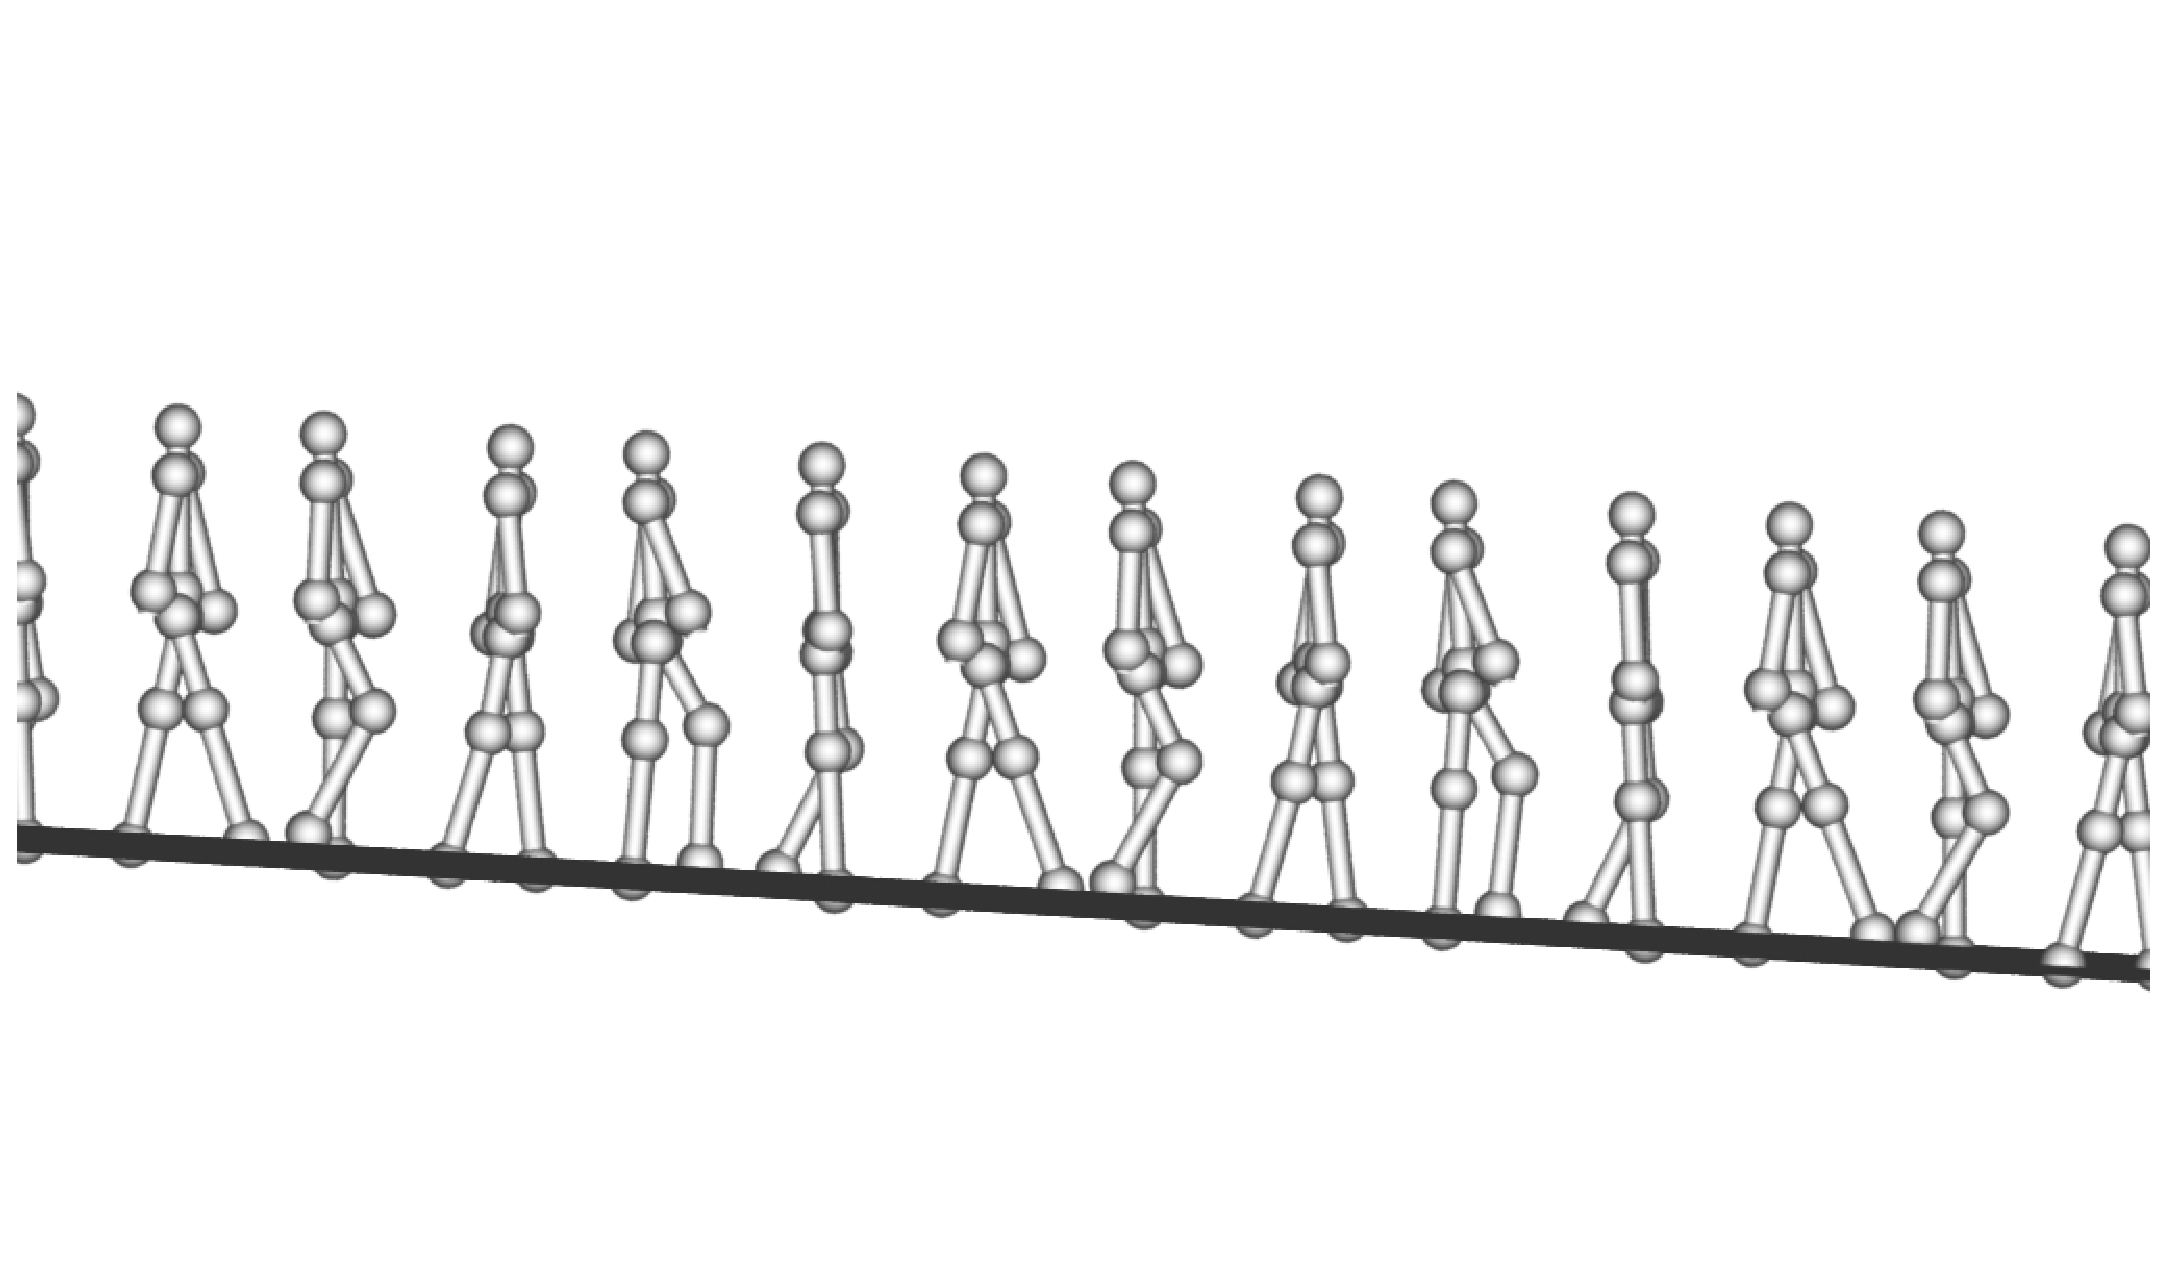
\includegraphics[width=0.7\textwidth]{LTLS7}
    \caption{gait of $\alpha_l=0.7$}
    \label{fig:lr2}
\end{center}
\end{figure}

\begin{figure}[!htbp]
  \begin{center}
      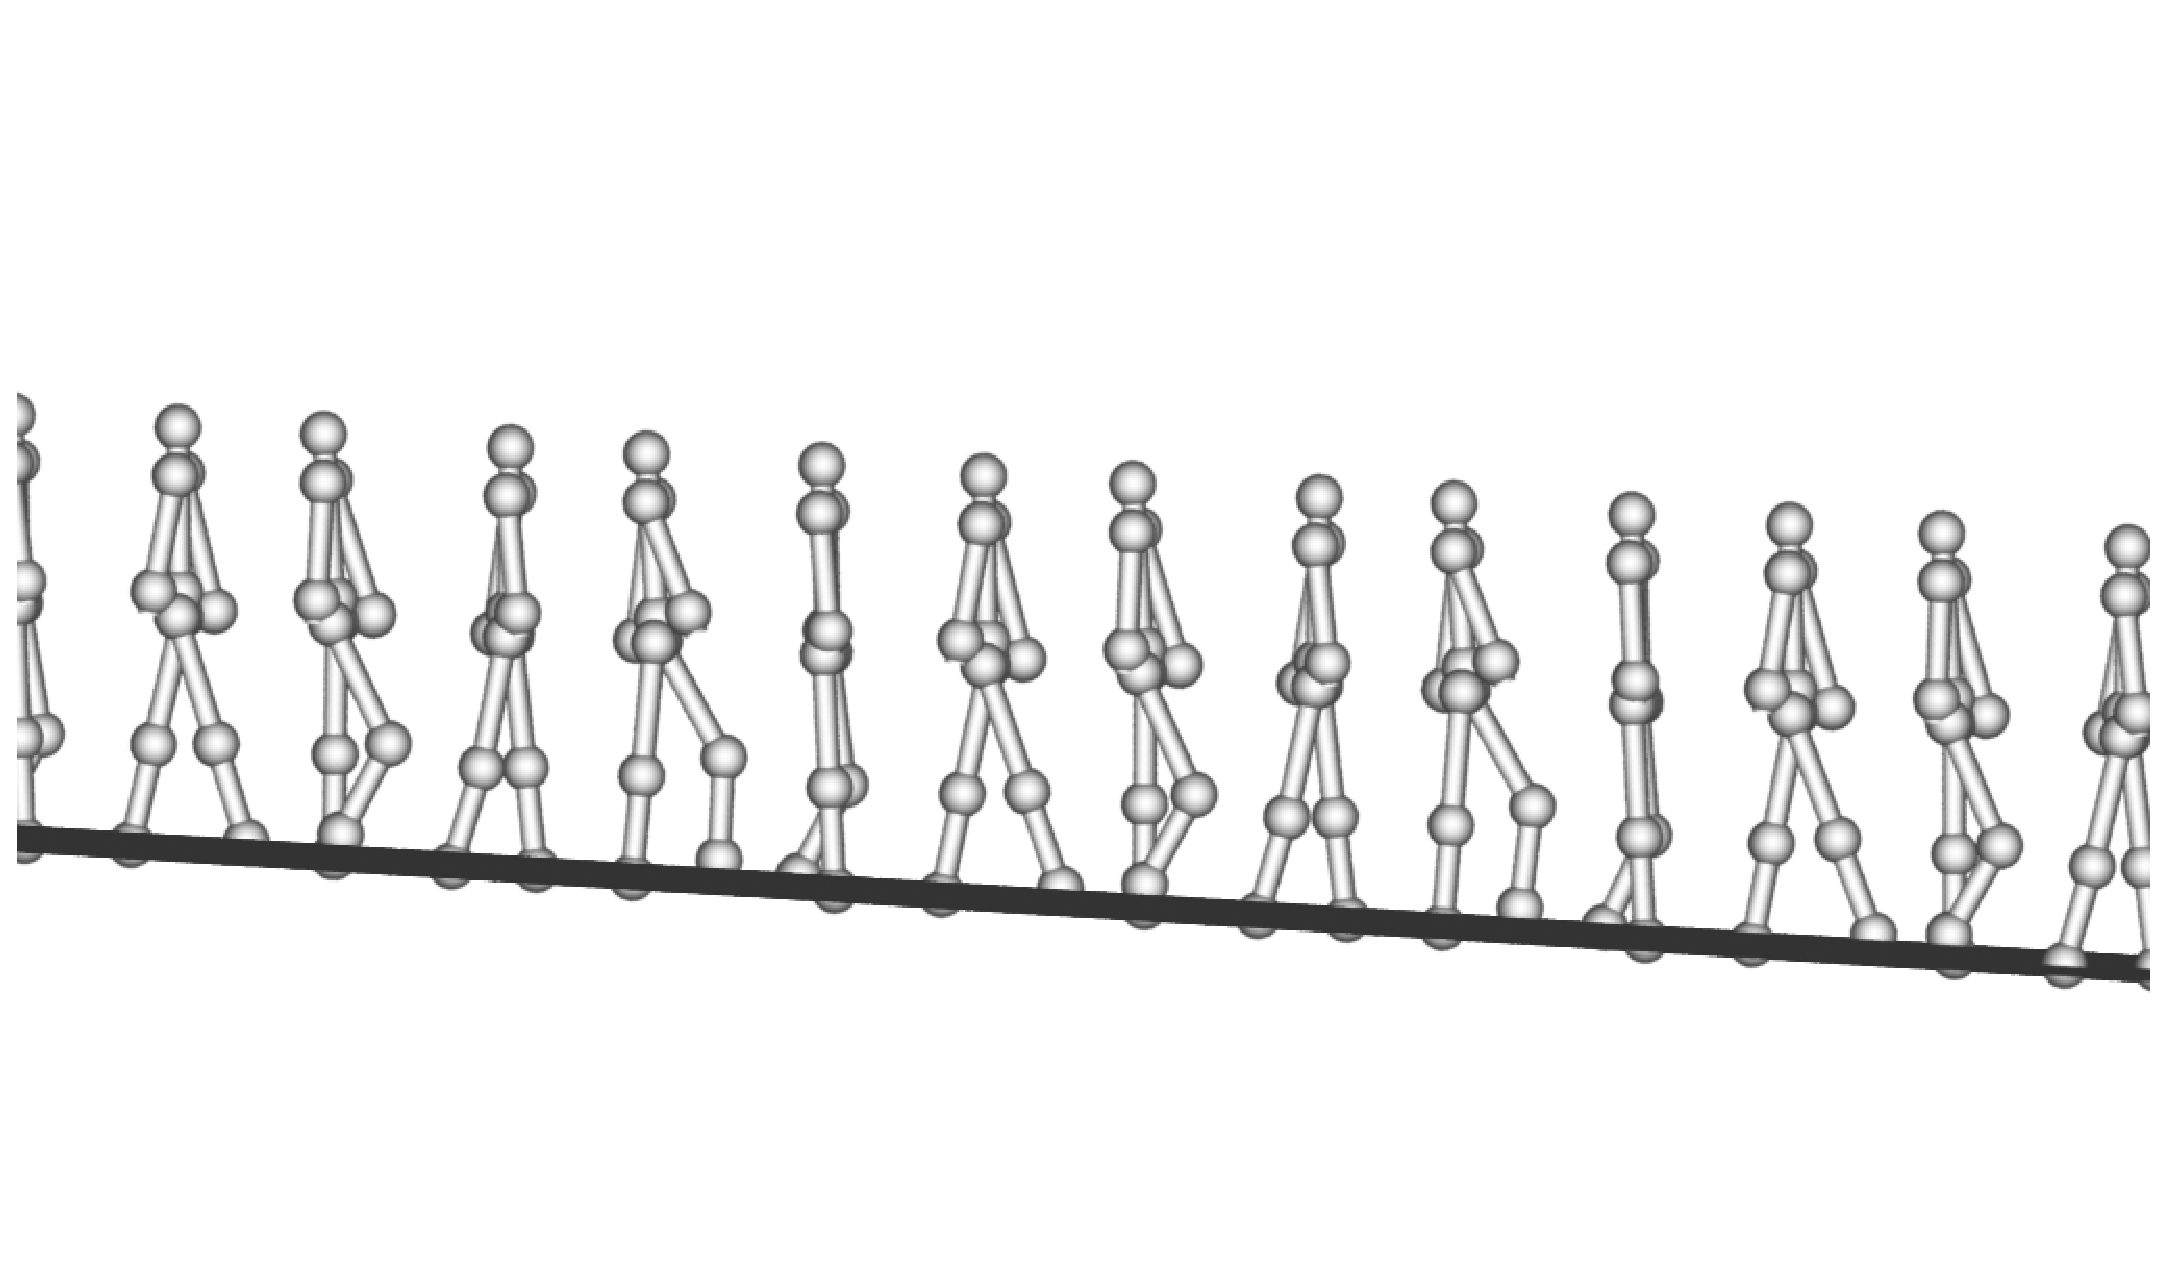
\includegraphics[width=0.7\textwidth]{LTLS13}
    \caption{gait of $\alpha_l=1.3$}
    \label{fig:lr3}
\end{center}
\end{figure}





\subsubsection*{Unbalanced Mass Ratio}
Also define the \emph{Unbalanced Mass Ration} 
\[
\alpha_b=\frac{\text{Left Leg Mass}}{\text{Right Leg Mass}}
\].


\begin{figure}[!htbp]
  \begin{center}
      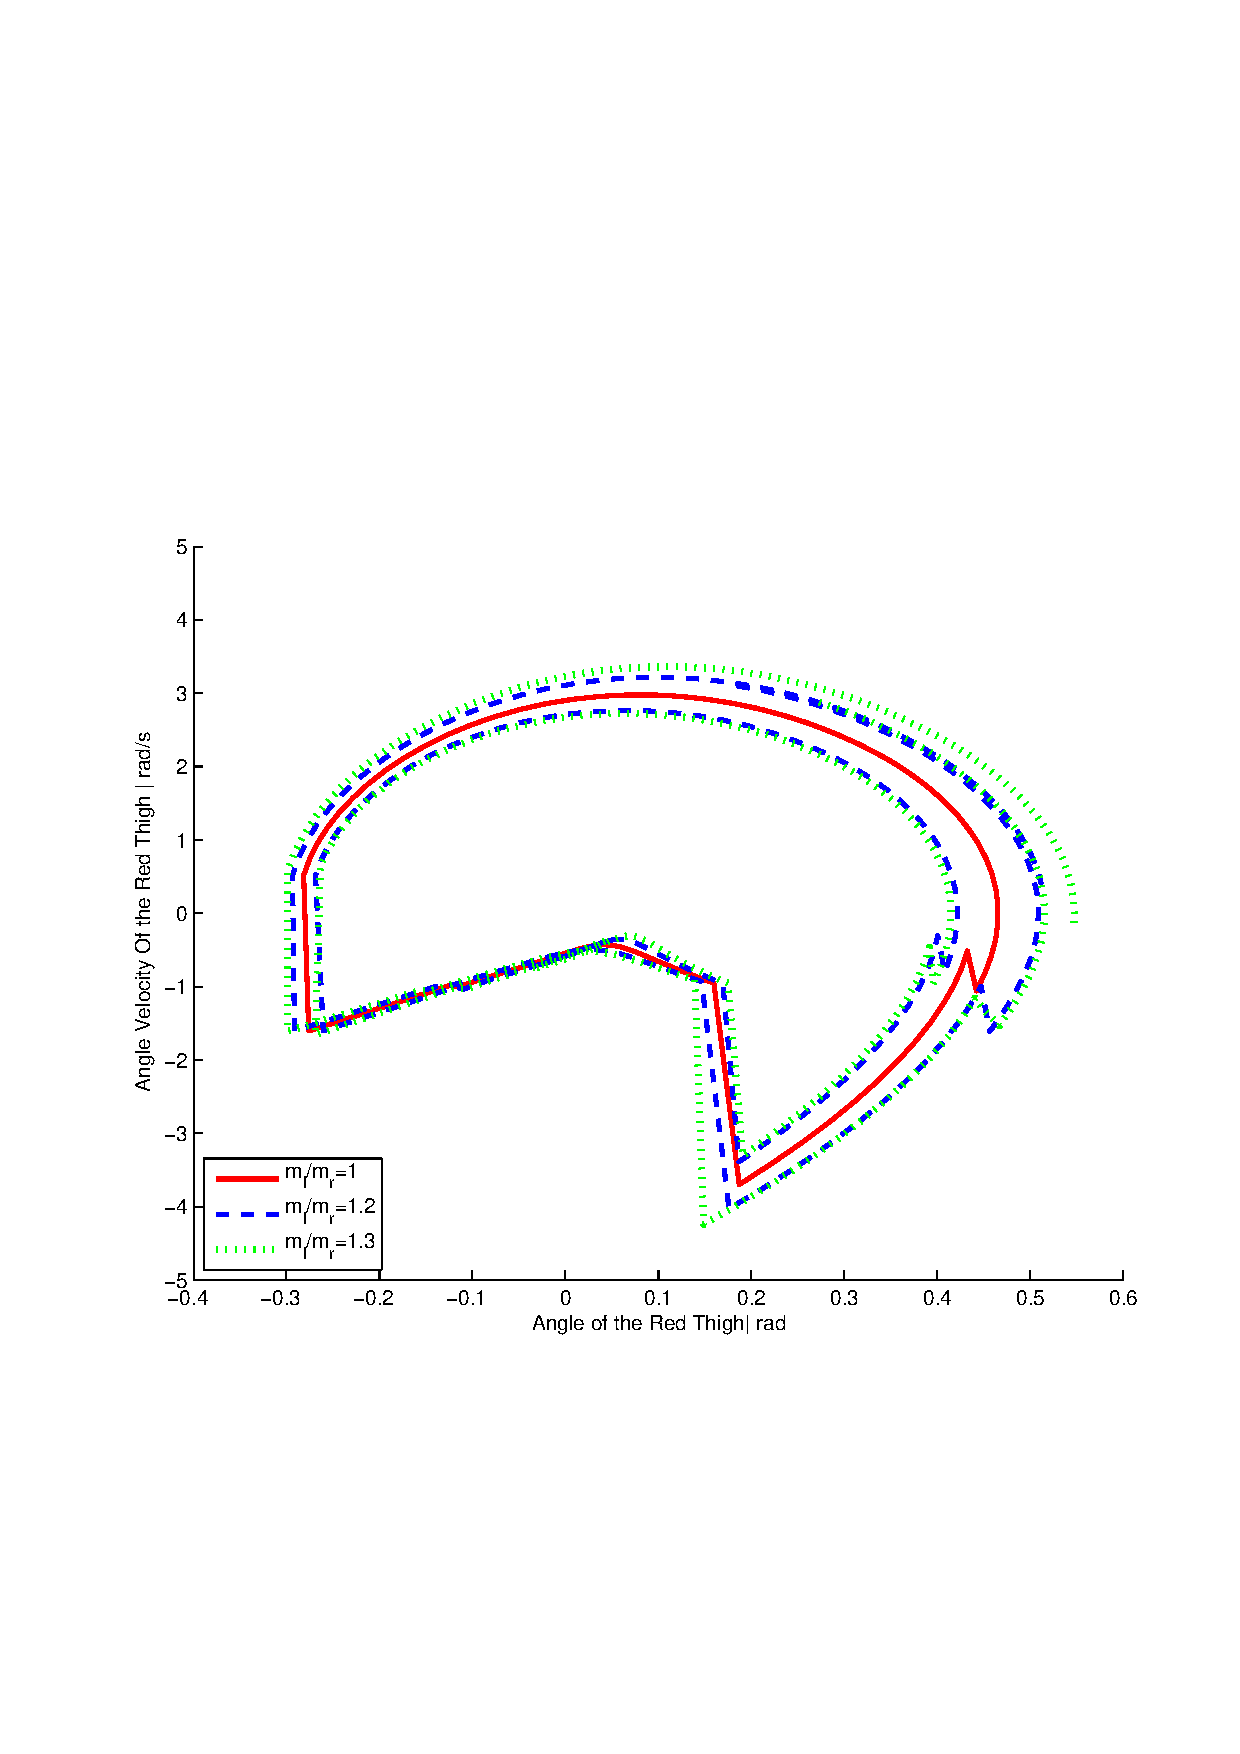
\includegraphics[width=0.7\textwidth]{DifferentLegMassLimitCircle}
    \caption{Different Leg Mass Stable Gaits}
    \label{fig:differentlr}
\end{center}
\end{figure}




\begin{figure}[!htbp]
  \begin{center}
      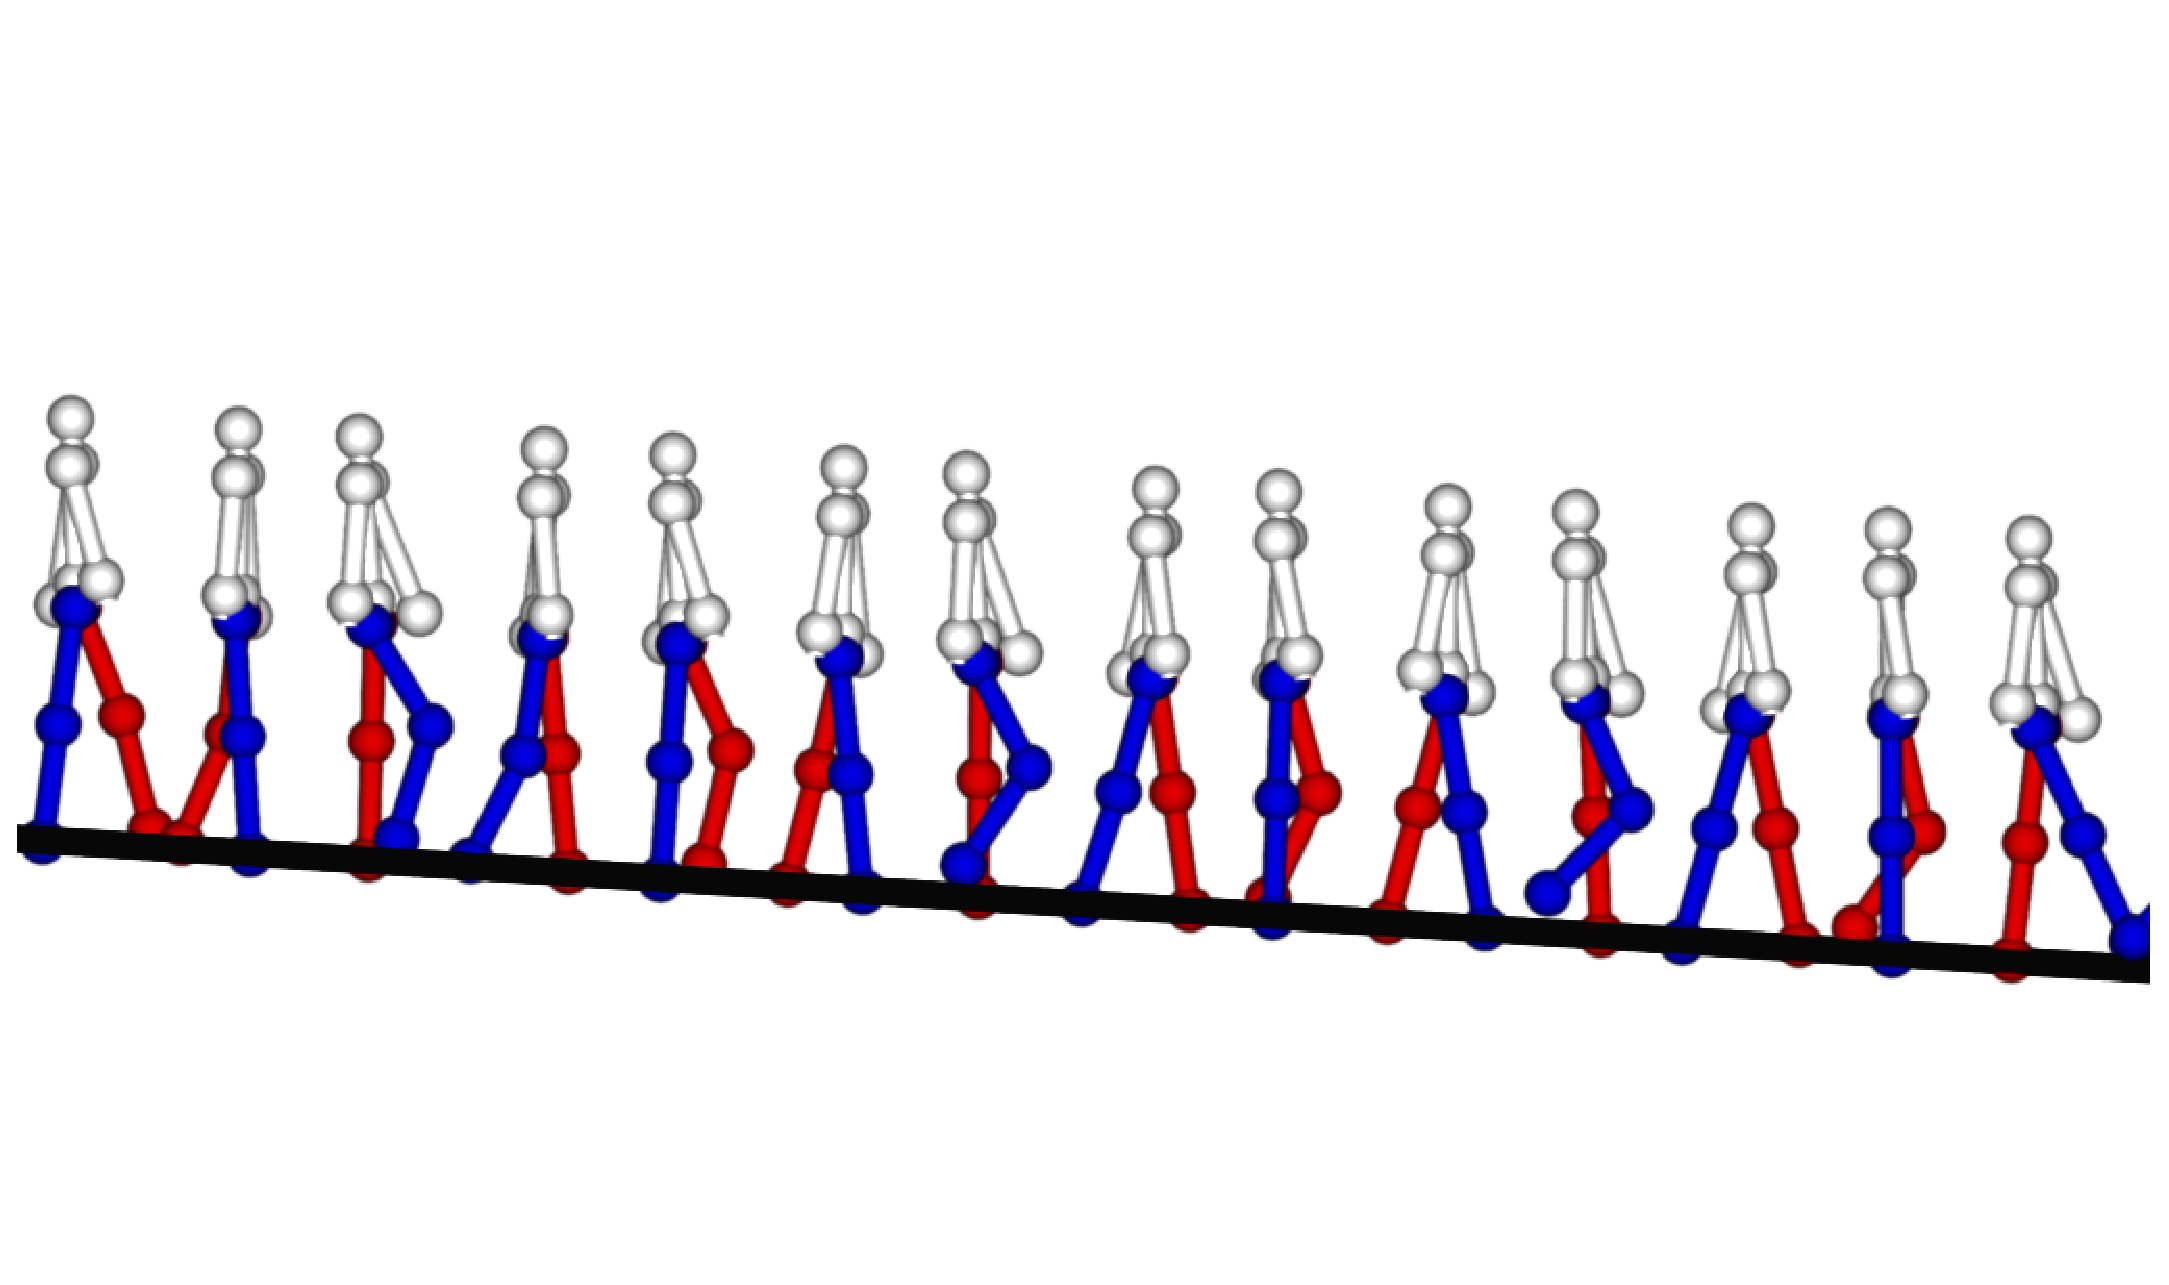
\includegraphics[width=0.7\textwidth]{MLMR130}
    \caption{Gait of $\alpha_b=1.3$}
    \label{fig:lm2}
\end{center}
\end{figure}
As shown in Figure~\ref{fig:differentlr},when $\alpha_b$ is increased, two legs sway differently and the limit circle is splitted.
Bigger $\alpha_b$  will result in cripple like gait, as shown in Figure~\ref{fig:lm2}



\subsubsection*{Different Slopes}
Usually, changing the slope may not seen as motion re targeting.
But in \moit, changing slope means changing the parameter of the dynamic equation, thus can be analysed in the same manner as changing body parameters.


Figure ~\ref{fig:diffslopes} shows the limit cycle of walking on different slopes.
For different slopes, entrainment maintains the limit cycle, but limit cycle changed its shape.
Different stable limit cycles are show in Figure ~\ref{fig:diffslopes}.
Basically, the bigger the slope, the bigger the step size, the higher the speed.
Slope changing has similar effects to energy scaling.



\begin{figure}[!htbp]
  \begin{center}
      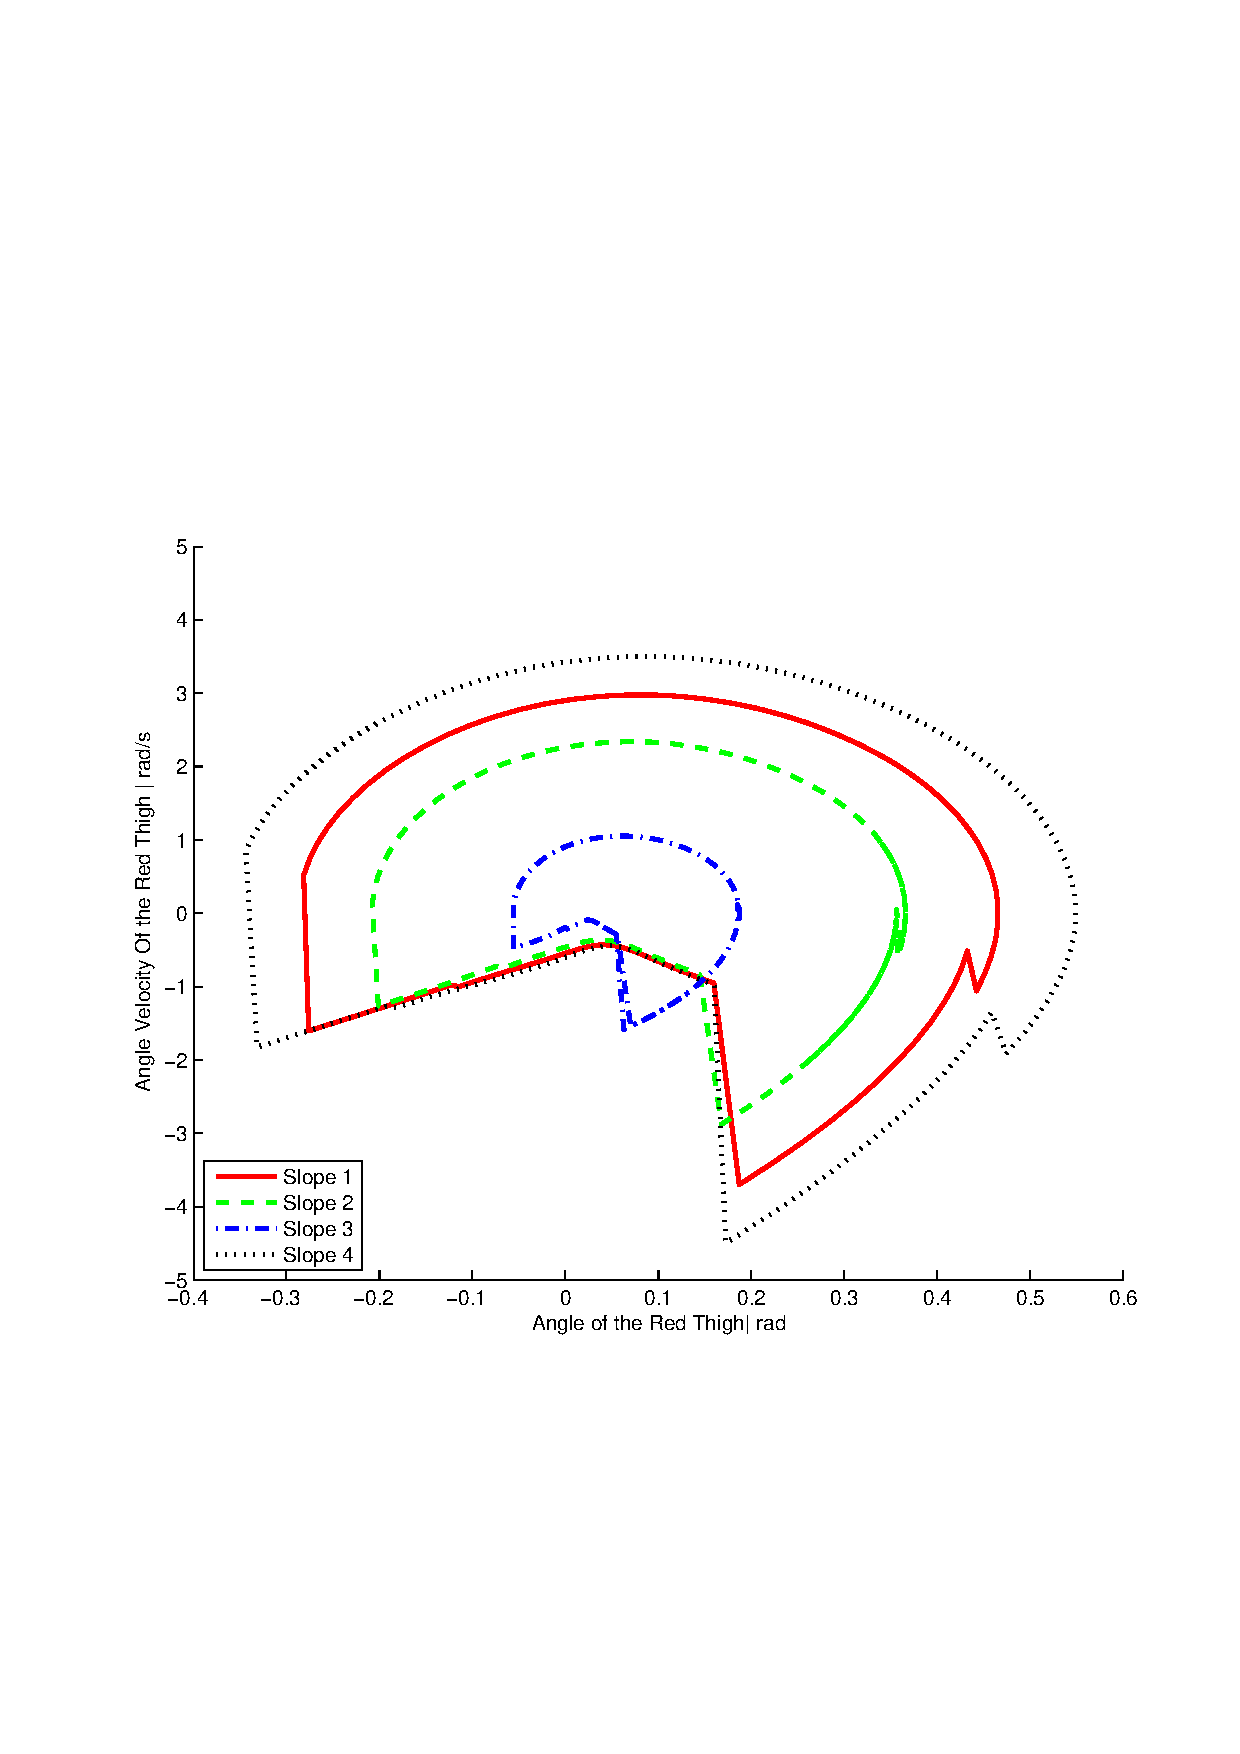
\includegraphics[width=0.7\textwidth]{DifferentSlope}
    \caption{different step size walking}
    \label{fig:diffslopes}
\end{center}
\end{figure}

Figure~\ref{fig:ss1},Figure~\ref{fig:ss2} and Figure~\ref{fig:ss3} show different gaits.

\begin{figure}[!htbp]
  \begin{center}
      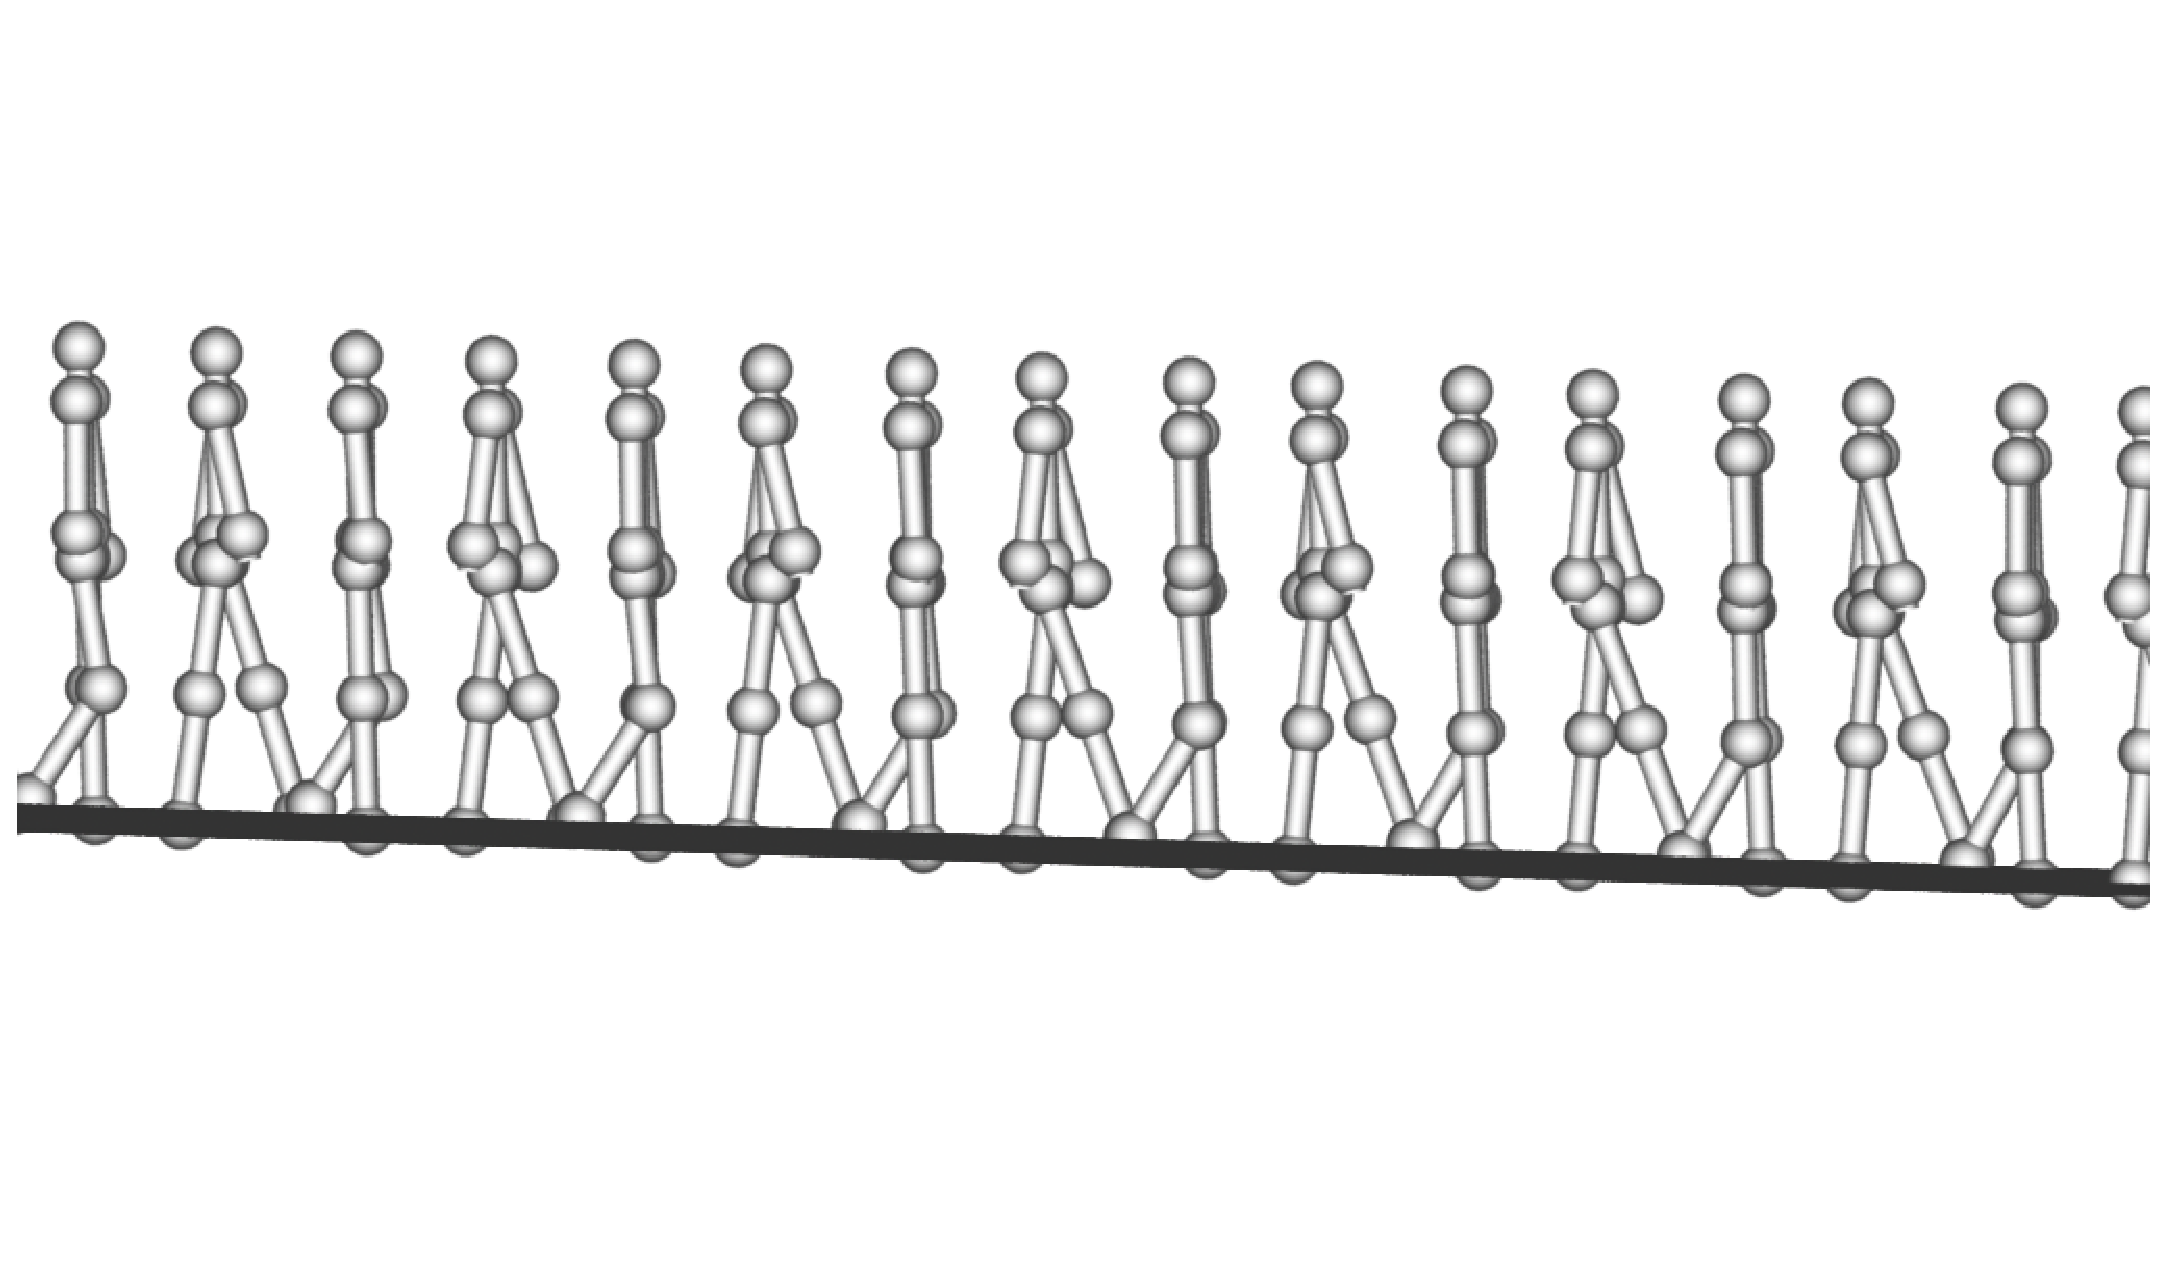
\includegraphics[width=0.7\textwidth]{Slope30}
    \caption{Gait On Slope 1} 
    \label{fig:ss1}
\end{center}
\end{figure}

\begin{figure}[!htbp]
  \begin{center}
      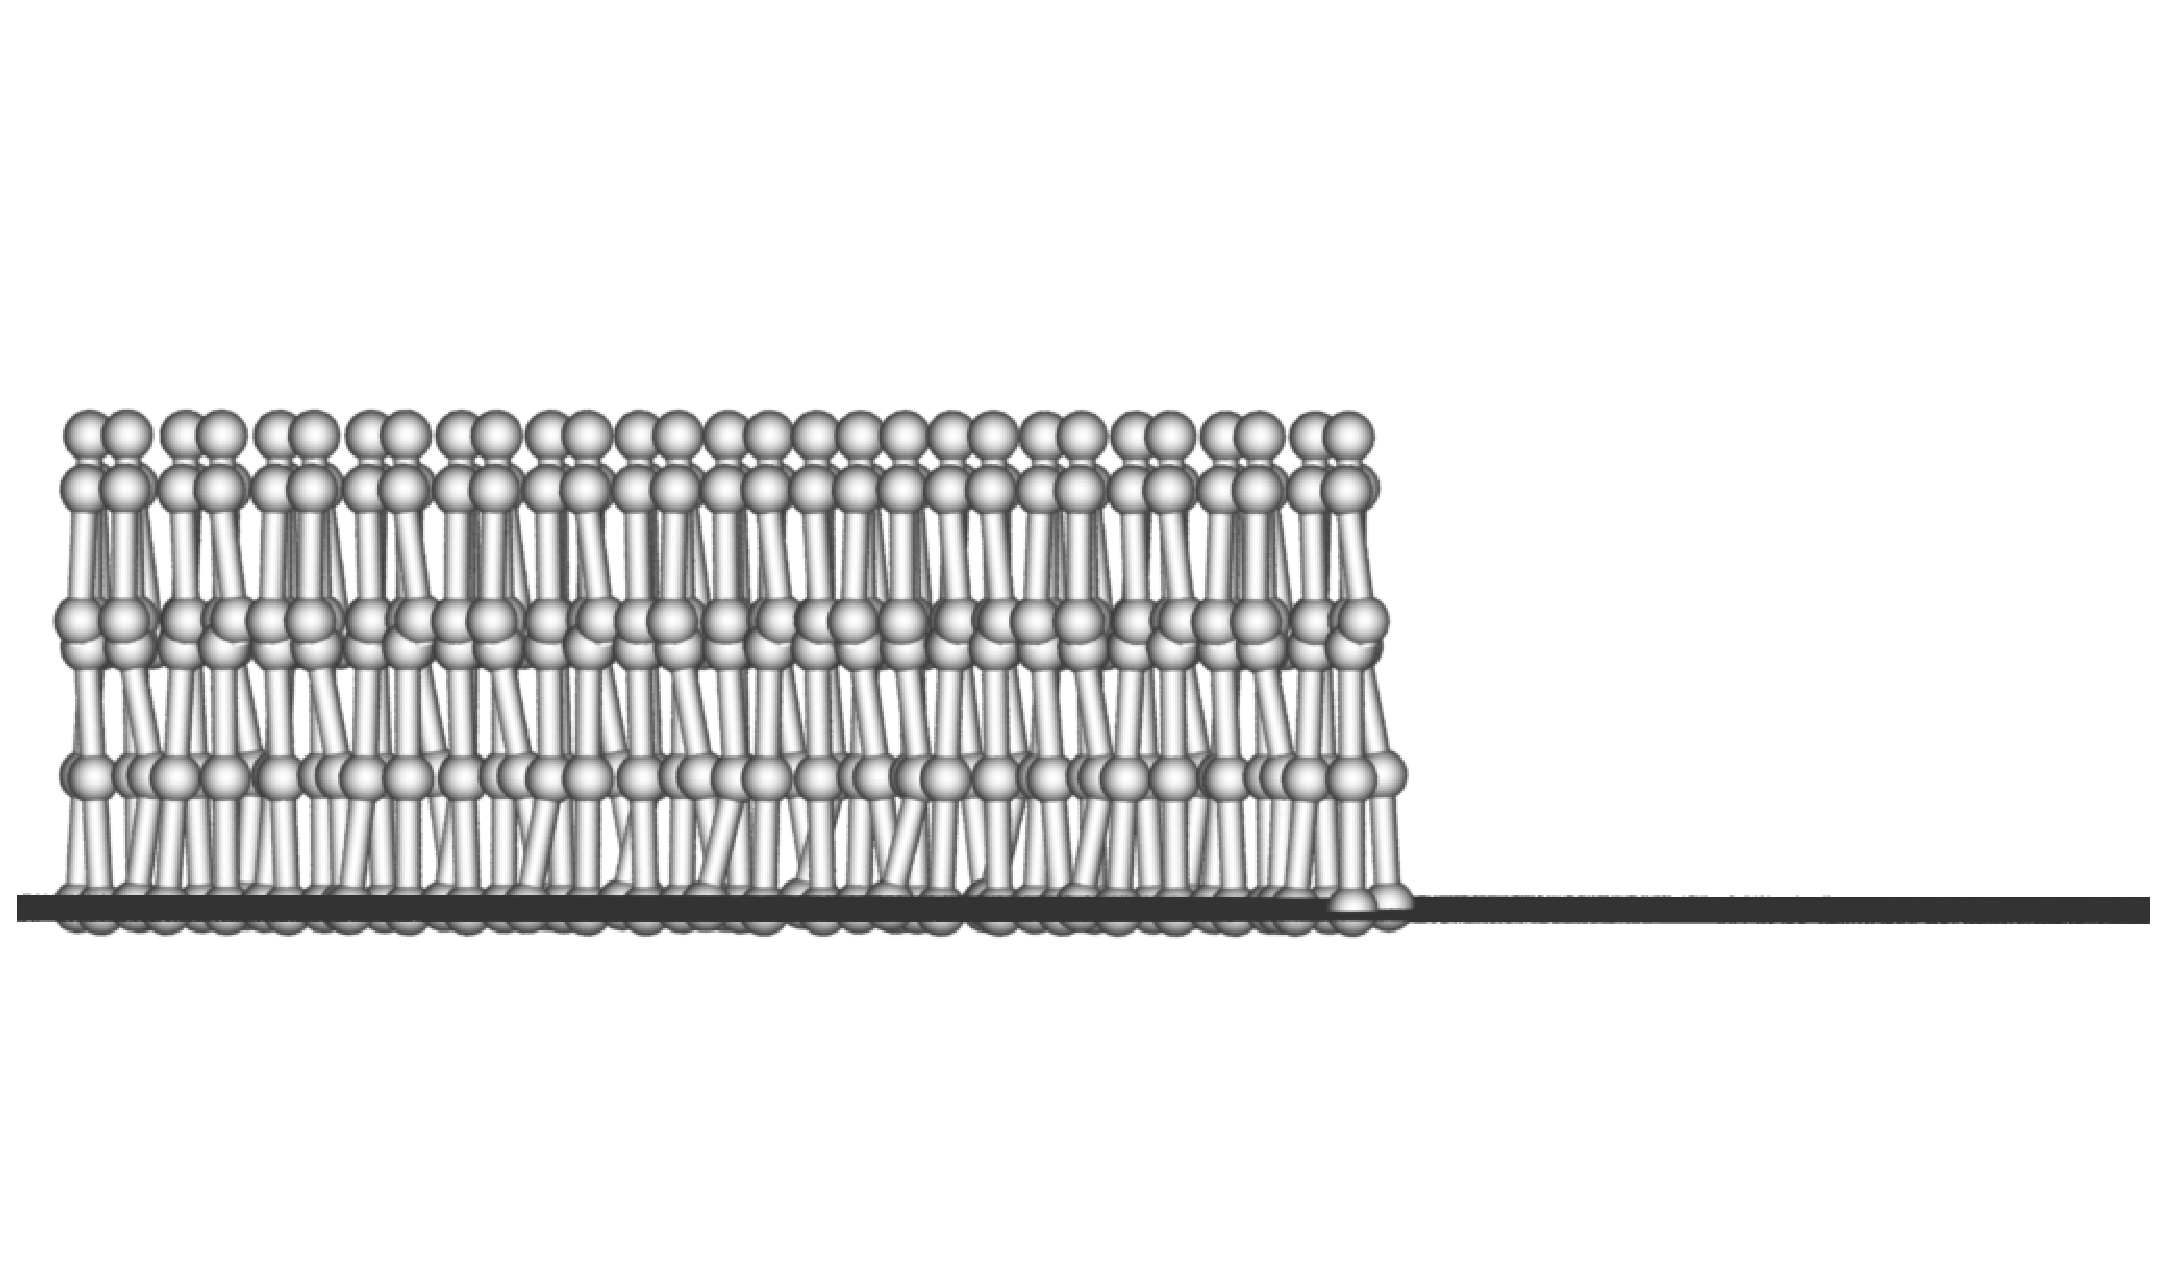
\includegraphics[width=0.7\textwidth]{Slope60}
    \caption{Gait On Slope 2}
    \label{fig:ss2}
\end{center}
\end{figure}

\begin{figure}[!htbp]
  \begin{center}
      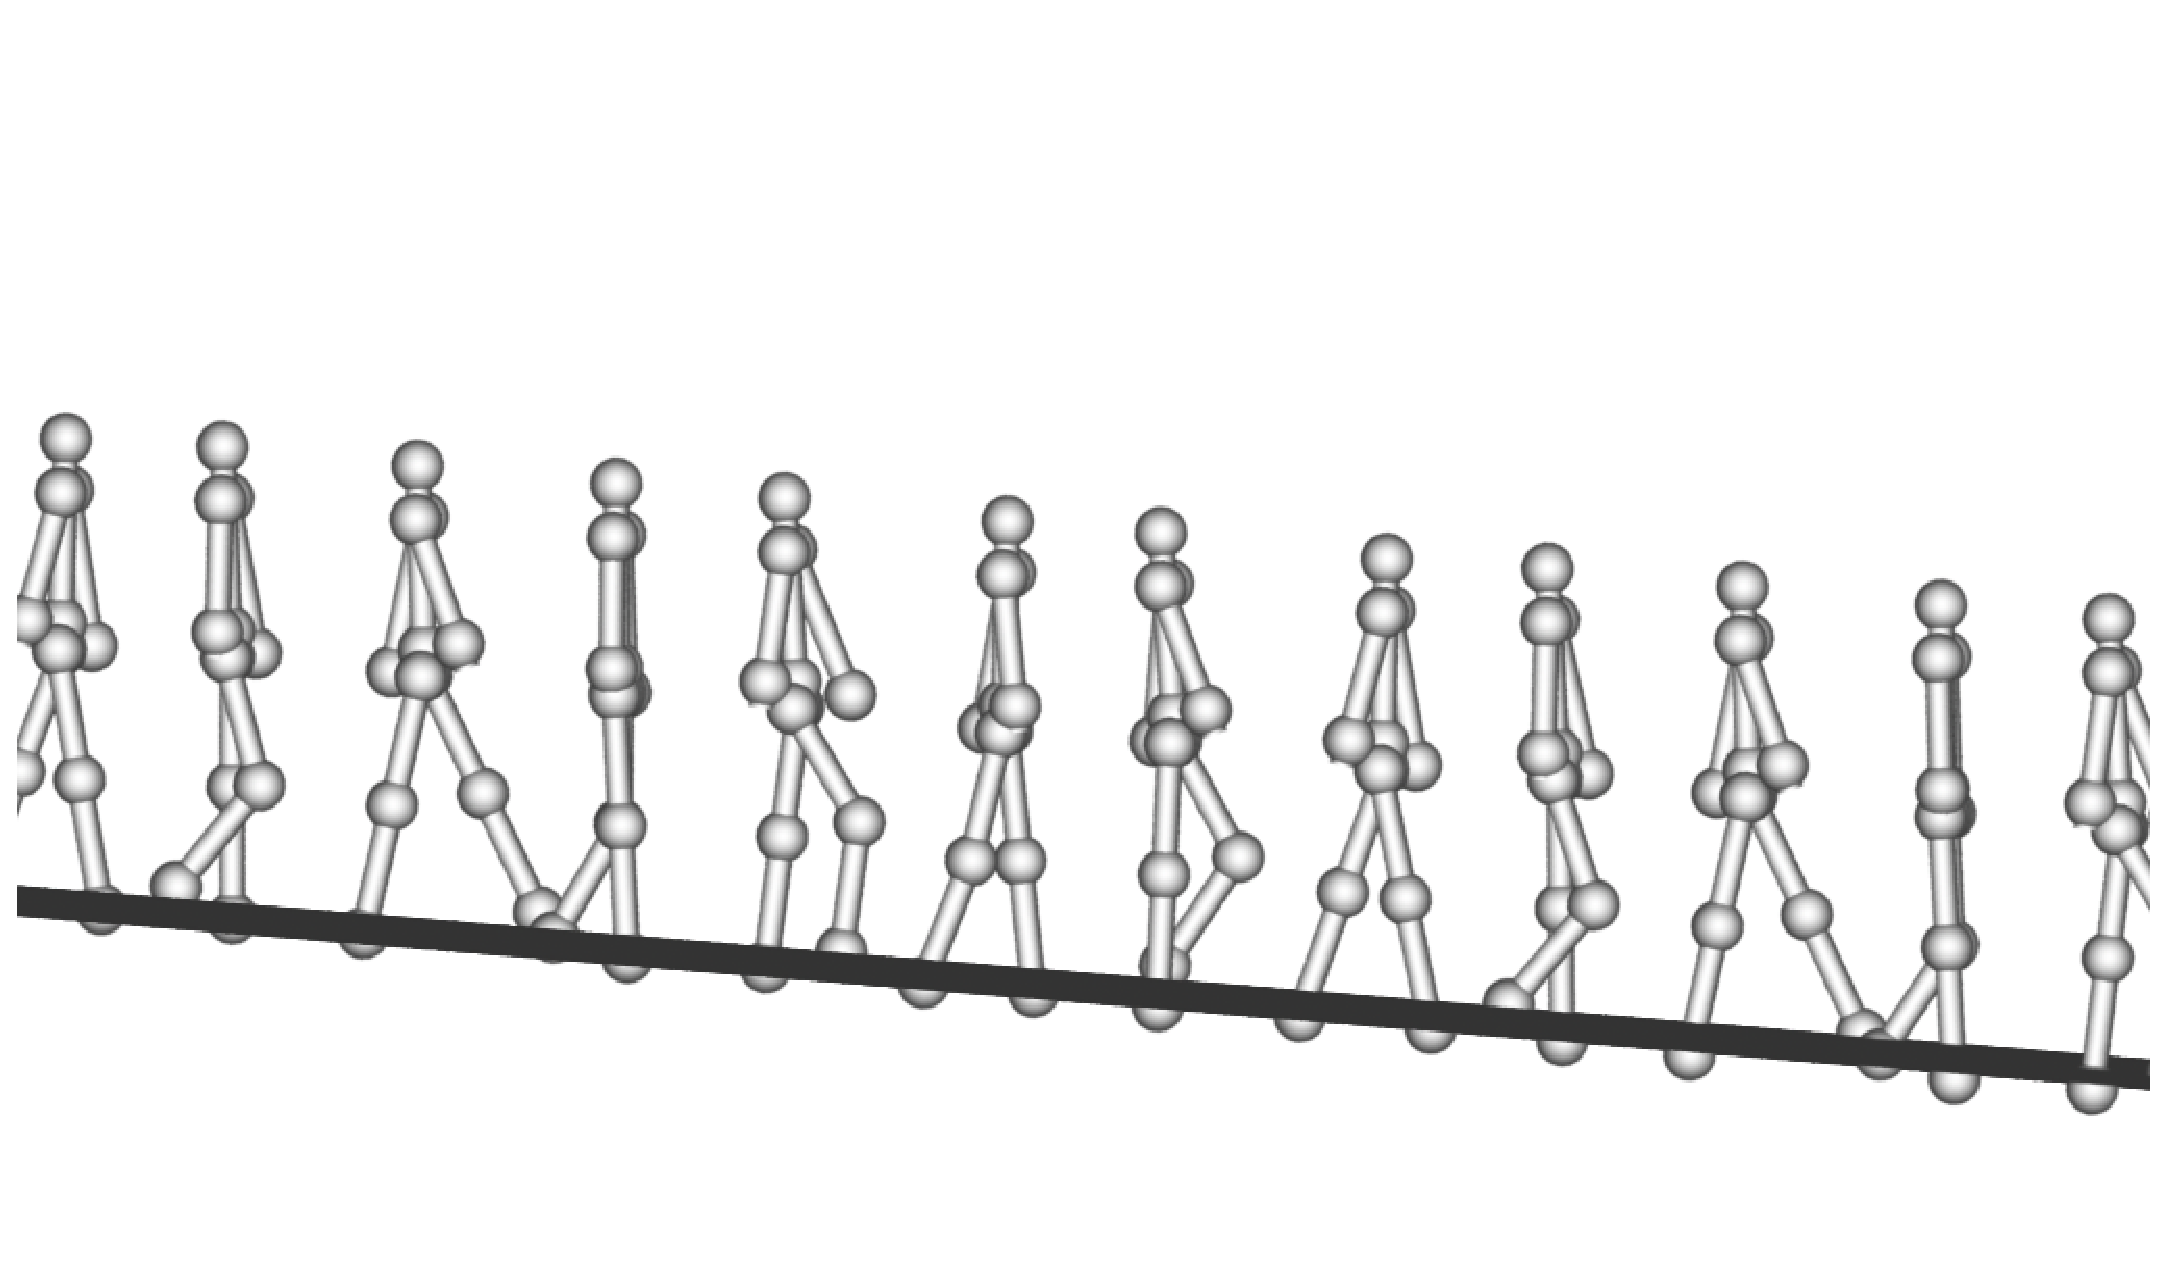
\includegraphics[width=0.7\textwidth]{Slope-20}
    \caption{Gait On Slope 3}
    \label{fig:ss3}
\end{center}
\end{figure}






\section{Local Motor Invariant Control}
Neural Oscillator boosts the stability.
Sometimes stability becomes a limitation in motion.
For the walking example, if the basin of attraction covers the whole space, then the passive walker can't walk up slope.
If put the walker walk up slope, after a few steps, the passive walker will begin to walk backward down slope,as shown in Figure~\ref{fig:localcontrolwalking}.
Also it is not convenient to adjust the speed of walking.




\begin{figure}[!htbp]
  \begin{center}
         $\begin{array}{cccc}
\includegraphics[width=1in]{UpFall/0001.eps}&
\includegraphics[width=1in]{UpFall/0051.eps}&
\includegraphics[width=1in]{UpFall/0101.eps}&
\includegraphics[width=1in]{UpFall/0151.eps}
\\
\includegraphics[width=1in]{UpFall/0201.eps}&
\includegraphics[width=1in]{UpFall/0251.eps}&
\includegraphics[width=1in]{UpFall/0301.eps}&
\includegraphics[width=1in]{UpFall/0351.eps}
\end{array}$
    \caption{Failure of walking upslope}
    \label{fig:localcontrolwalking}
\end{center}
\end{figure}

Local Motor Invariant provides a mechanism to adapt motion according to the environment and application specific purpose. 
For the bipedal walking, Group actions provides a mechanism to adjust the walking slope and walking speed in precision.




\subsubsection{Group Actions}

Equation~\ref{eq:localcontrolwalking} describes walking with local control.
\begin{equation}
\label{eq:localcontrolwalking}
M(\mathbf{q}) \ddot{\mathbf{q}} + C(\mathbf{q,\qd})\dot{\mathbf{q}} + N(\mathbf{q}) = \ulocal
\end{equation}




Lie group actions are developed for two types of symmetry.
\begin{itemize}

\HiItem{Offset Action}.
Offset Action moves the phase plot horizontally.
This will make the passive walking on terrain of different slope.
For the bipedal walking, the offset action is:
\[
\ulocal=N(q)-N(q+\ep)
\]
\HiItem{Speed Action}
Speed Action maintains the walking gait, but modifies the walking speed.
The local control is:
\[  
\ulocal=(1-\ep^2)N
\]
\end{itemize}

The original system does not have energy scaling symmetry.
Energy Scaling is approximated by a combined method discussed later.

Figure~\ref{fig:walkliegroupphase} demonstrates different phase plot after applying lie group actions.
The red one is the original limit cycle.
Green ones are applied speed actions and blue ones are applied local transform action.


\begin{figure}[!htbp]
  \begin{center}
     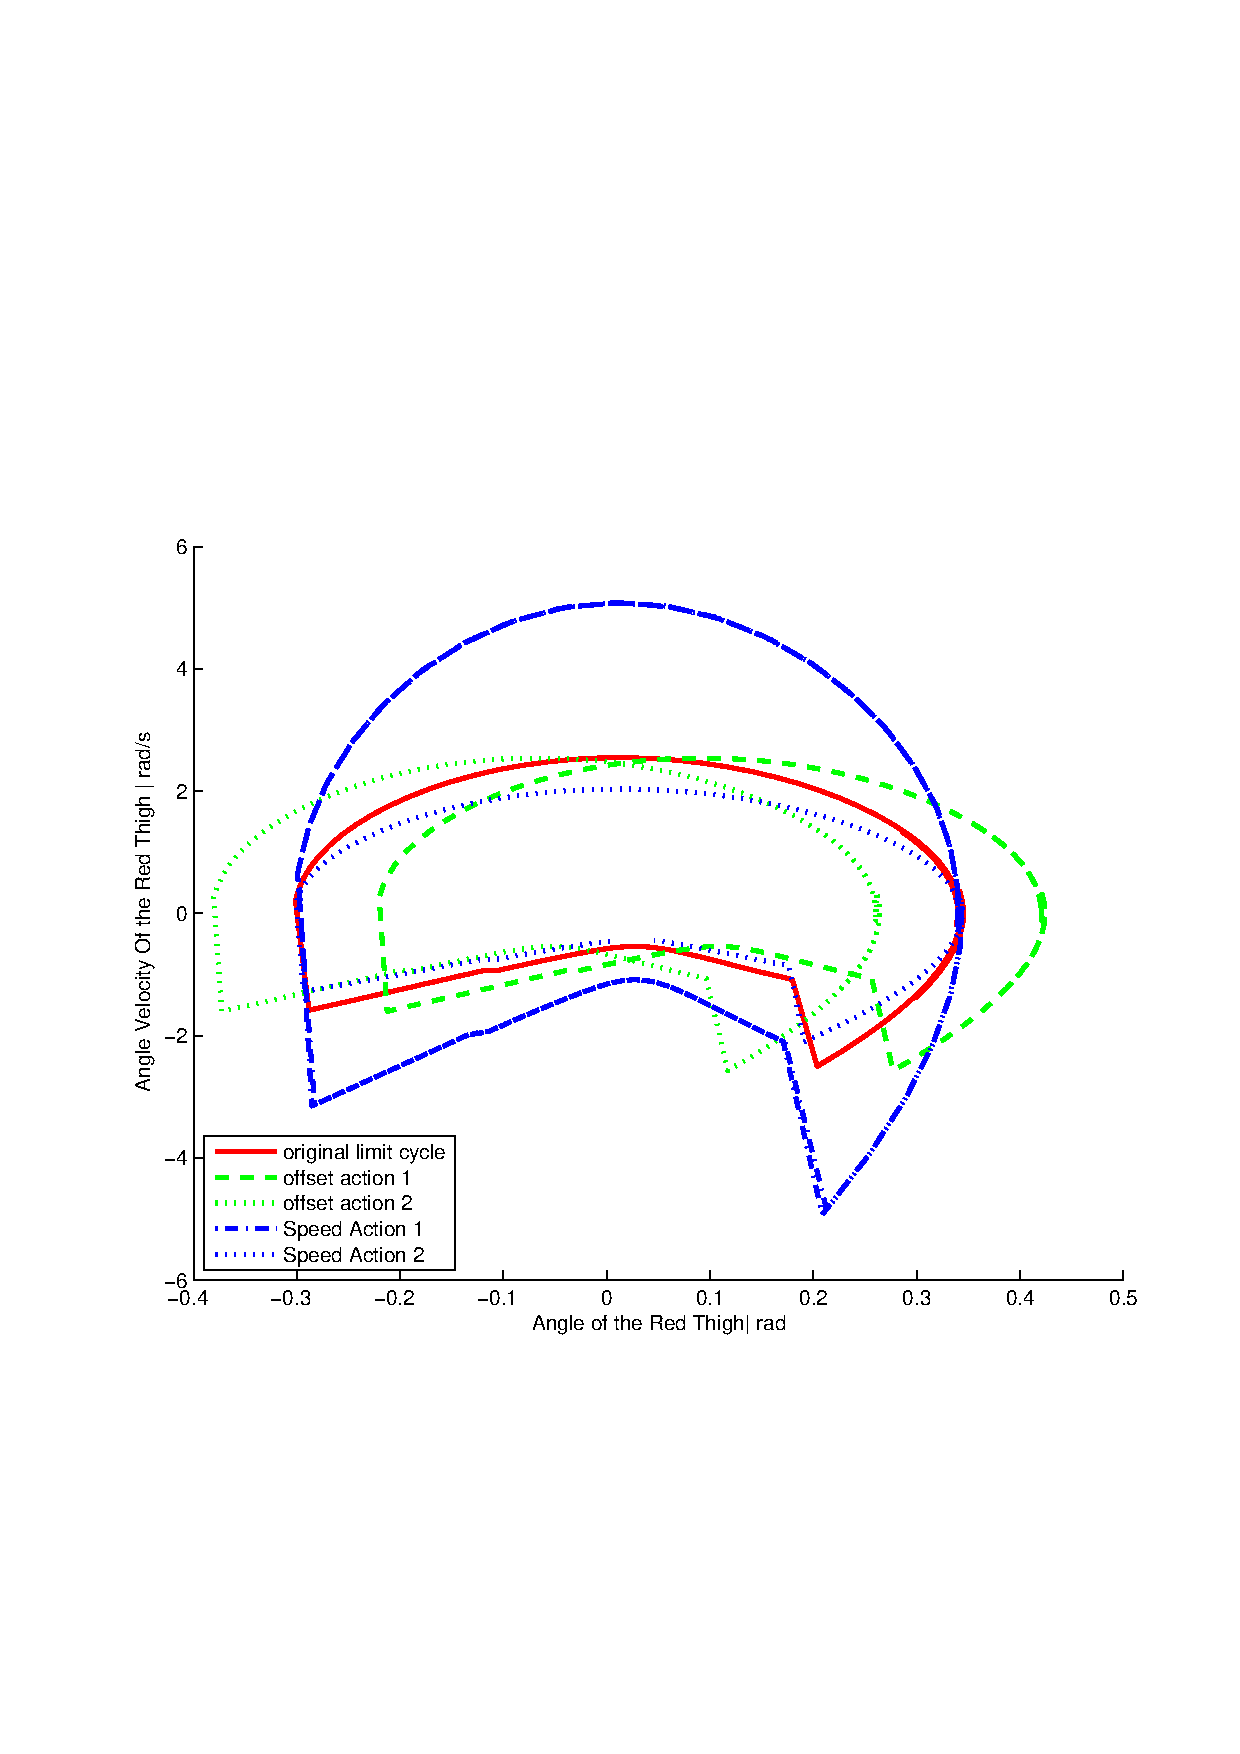
\includegraphics[width=0.7\textwidth]{LieGroupAction}
    \caption{Lie Group Actions on the Phase Plot}
    \label{fig:walkliegroupphase}
\end{center}
\end{figure}


By applying the offset action,   the passive walker to walk up slope, as shown in Figure~\ref{fig:liegroupupslope}
\begin{figure}[!htbp]
  \begin{center}
      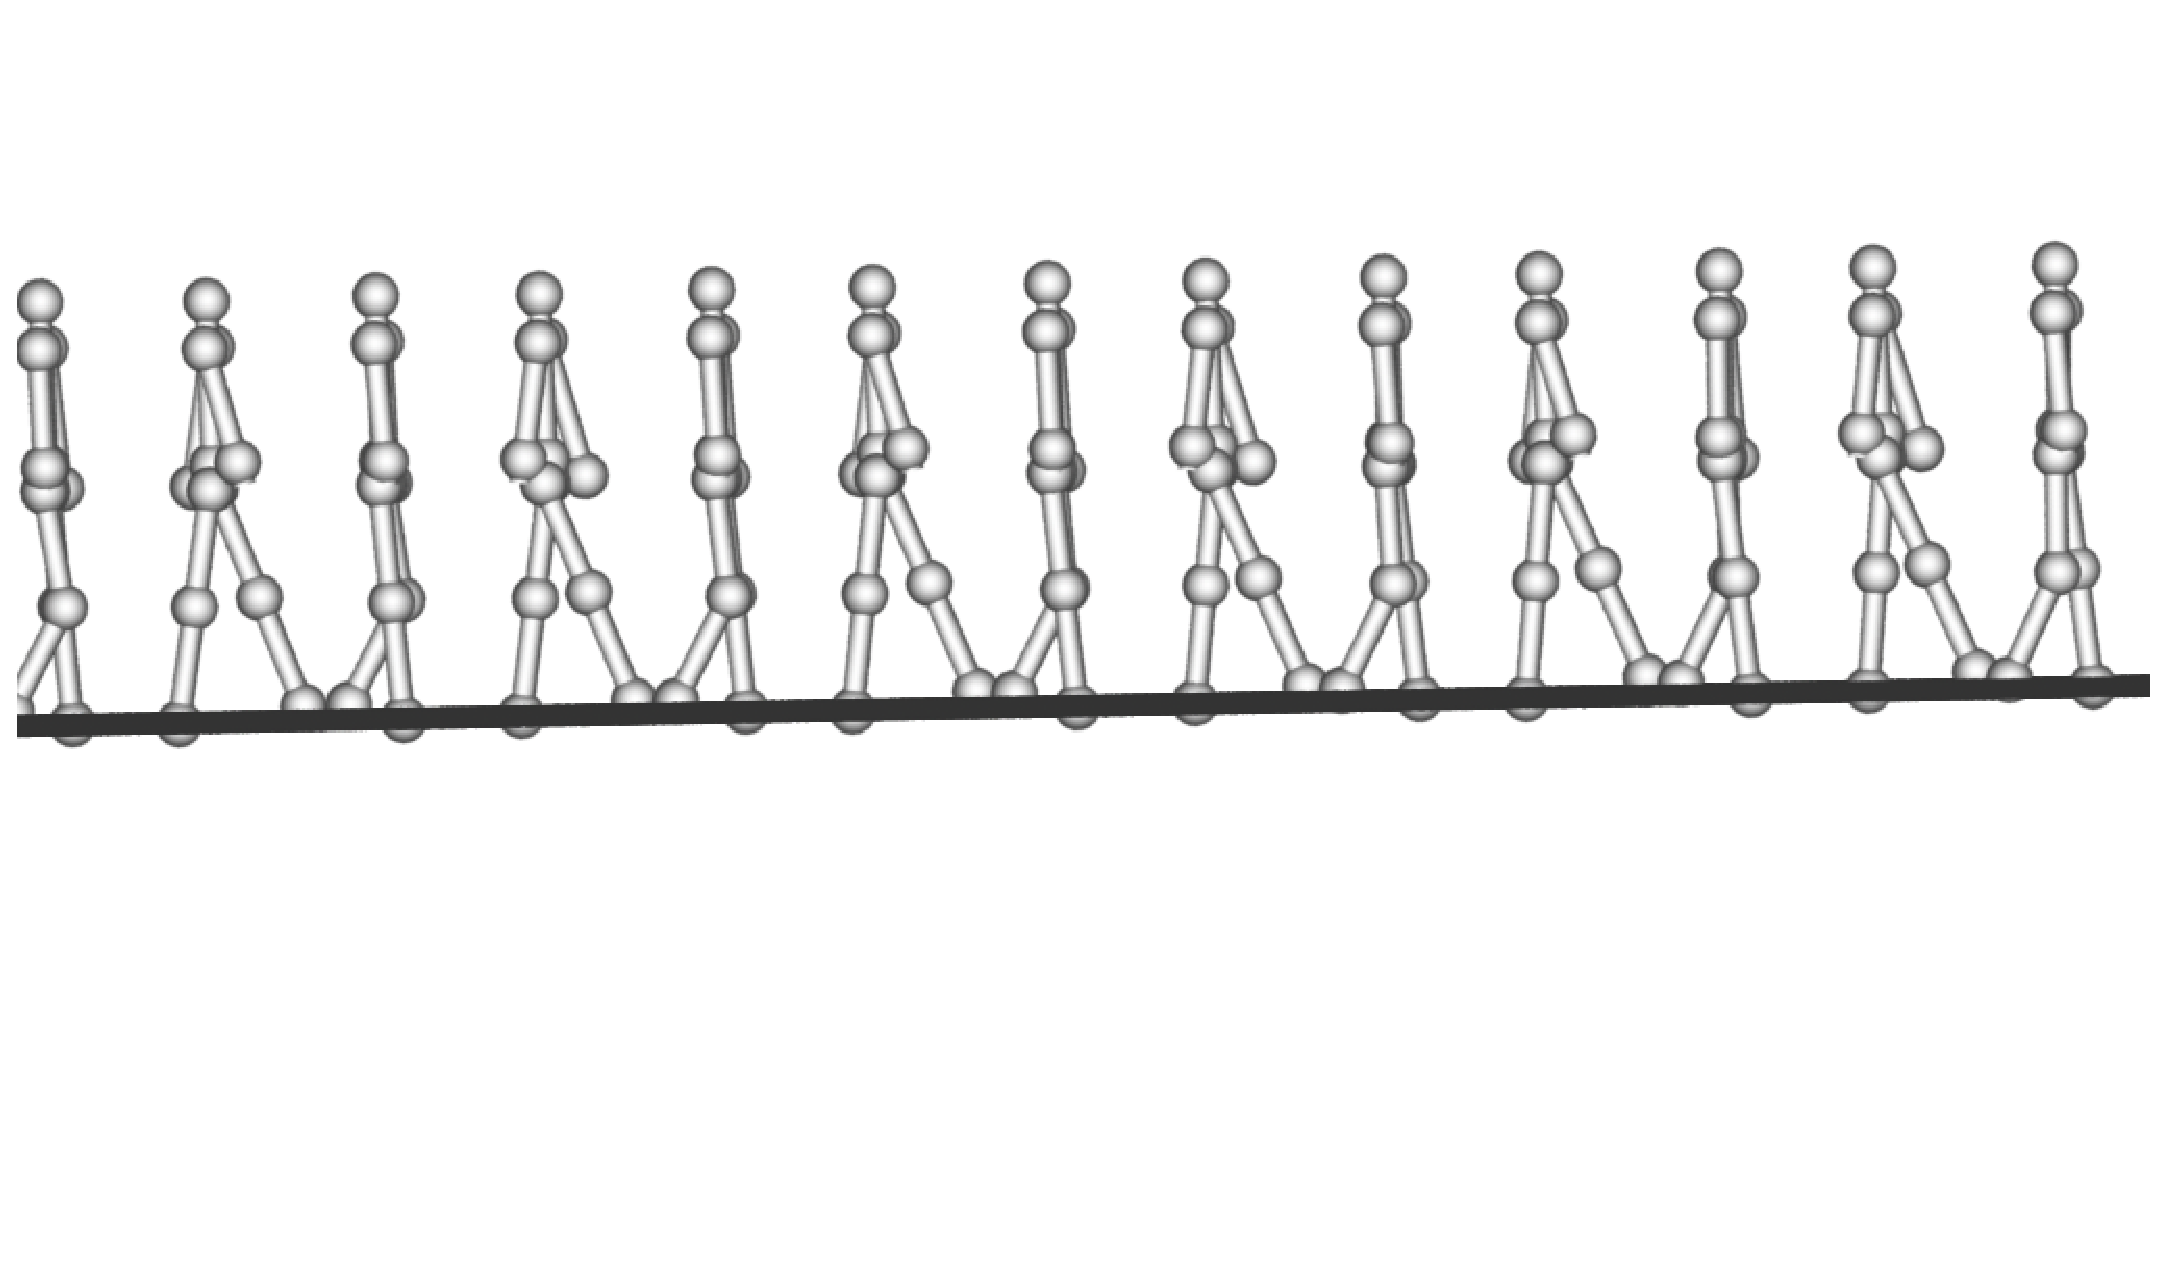
\includegraphics[width=0.7\textwidth]{LieUpslope}
    \caption{Up slope Gait Generate by Lie Group offset Action}
    \label{fig:liegroupupslope}
\end{center}
\end{figure}

\section{Application of Combined Method}
Global Motor Invariant Control boosts the walking stability, but sometimes  the result motion does not meet application's needs.
Local Motor Invariant Control can adapt the walking to application purpose, but it can't boost the stability.
Combining the two controllers make it possible to take advantages of the two methods.

The combined method is shown by Equation~\ref{eq:combinedcontrolwalking}
\begin{equation}
\label{eq:combinedcontrolwalking}
M(\mathbf{q}) \ddot{\mathbf{q}} + C(\mathbf{q,\qd})\dot{\mathbf{q}} + N(\mathbf{q}) = D\uout+\ulocal
\end{equation}

In applications, animator can generate different gaits through  adjusting neural oscillator and the body parameters, then transform the different gaits by lie group actions.
For animators, this method is efficient, natural looking and easy to use.

Such combinations will achieve unlimited variations of gaits.
In the following, we shown how some gaits variation can be achieved in this manner. 

\subsection{Step Size Adjust}
The first example shows how a character can adjust his step size realistically.



When the character walks down different slopes, steeper slope will result in a bigger step size as shown in Figure~\ref{fig:diffslopes}. 
if Offset Lie Group actions is applied, then we can transform the gait of different slope on the plane, we can achieve different step gait on the plane.

Figure~\ref{fig:differentstepsizeonplaine} shows limit cycles of the different step size gaits on the plane.
\begin{figure}[!htbp]
  \begin{center}
      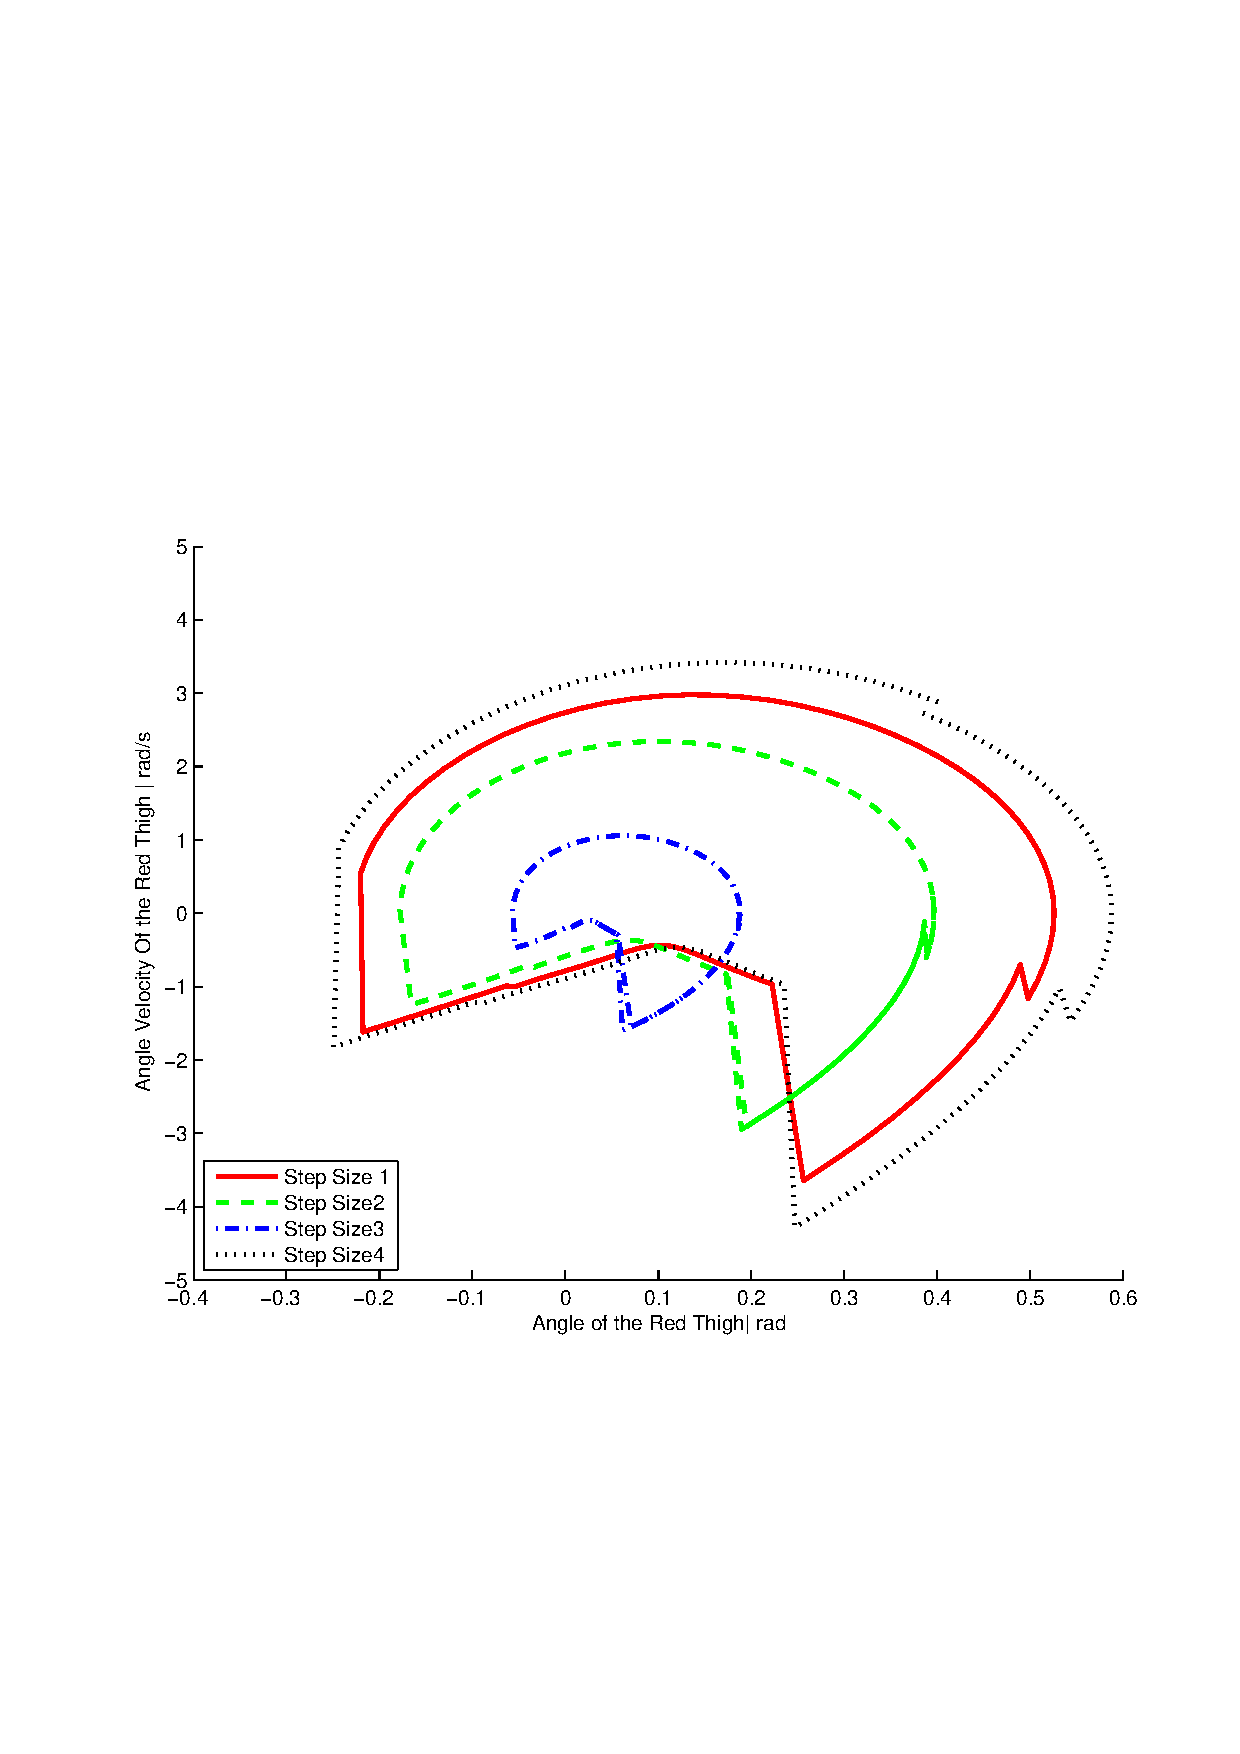
\includegraphics[width=0.7\textwidth]{DifferentStepSizeWalking}
    \caption{Limit Cycles of gaits of different step size}
    \label{fig:differentstepsizeonplaine}
\end{center}
\end{figure}


And the different gaits are shown in Figure~\ref{fig:ssp1},Figure~\ref{fig:ssp2},Figure~\ref{fig:ssp3}.
\begin{figure}[!htbp]
  \begin{center}
      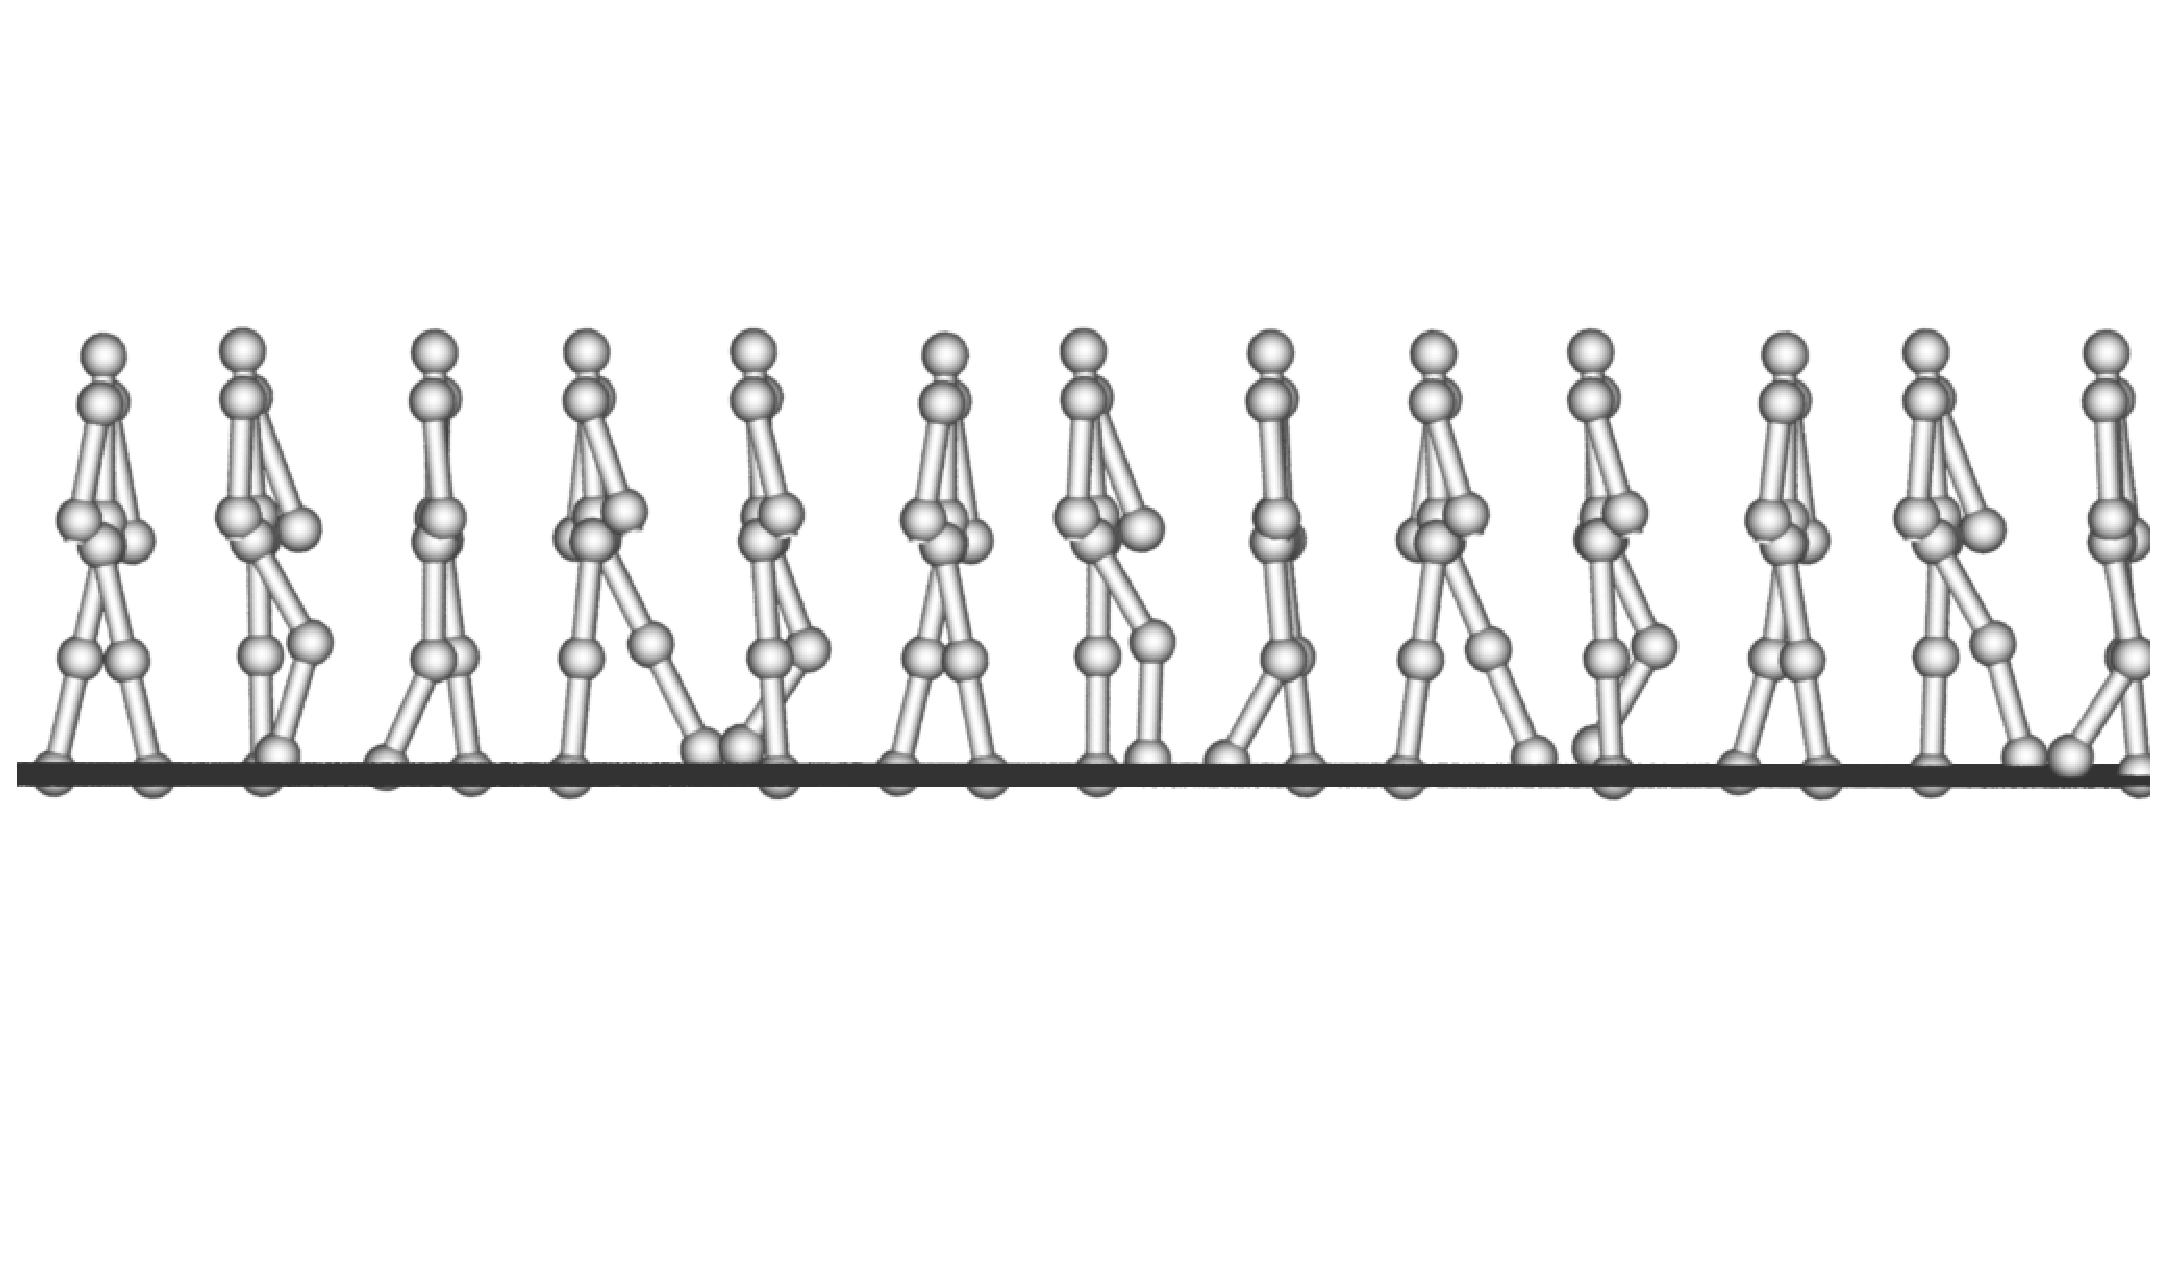
\includegraphics[width=0.7\textwidth]{stepsize1}
    \caption{gait with stepsize 1}
    \label{fig:ssp1}
\end{center}
\end{figure}

\begin{figure}[!htbp]
  \begin{center}
      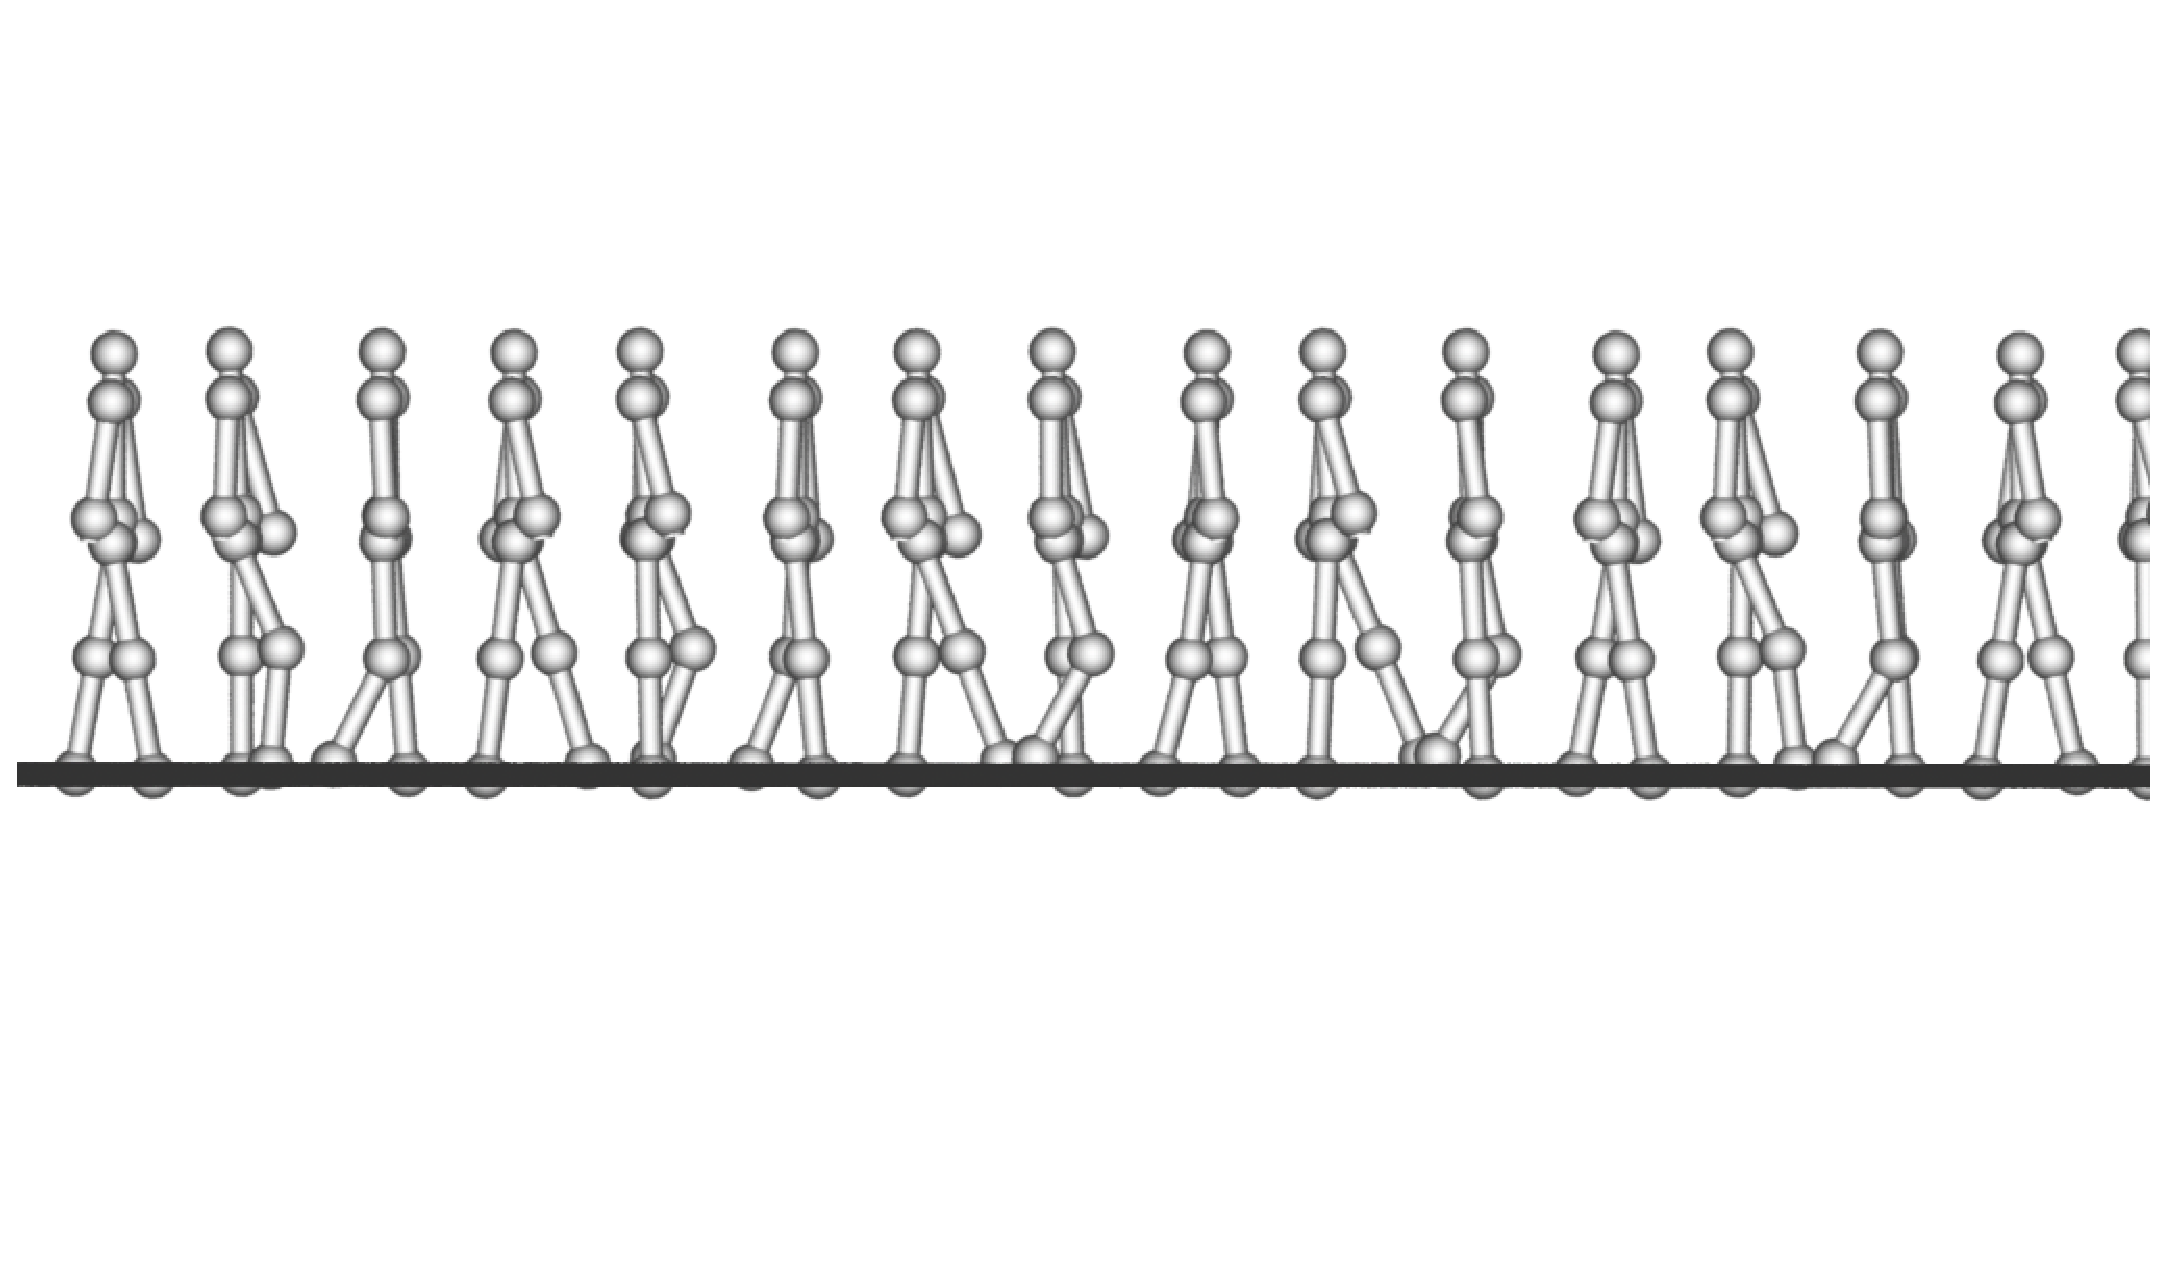
\includegraphics[width=0.7\textwidth]{stepsize2}
    \caption{gait with stepsize 2}
    \label{fig:ssp2}
\end{center}
\end{figure}

\begin{figure}[!htbp]
  \begin{center}
      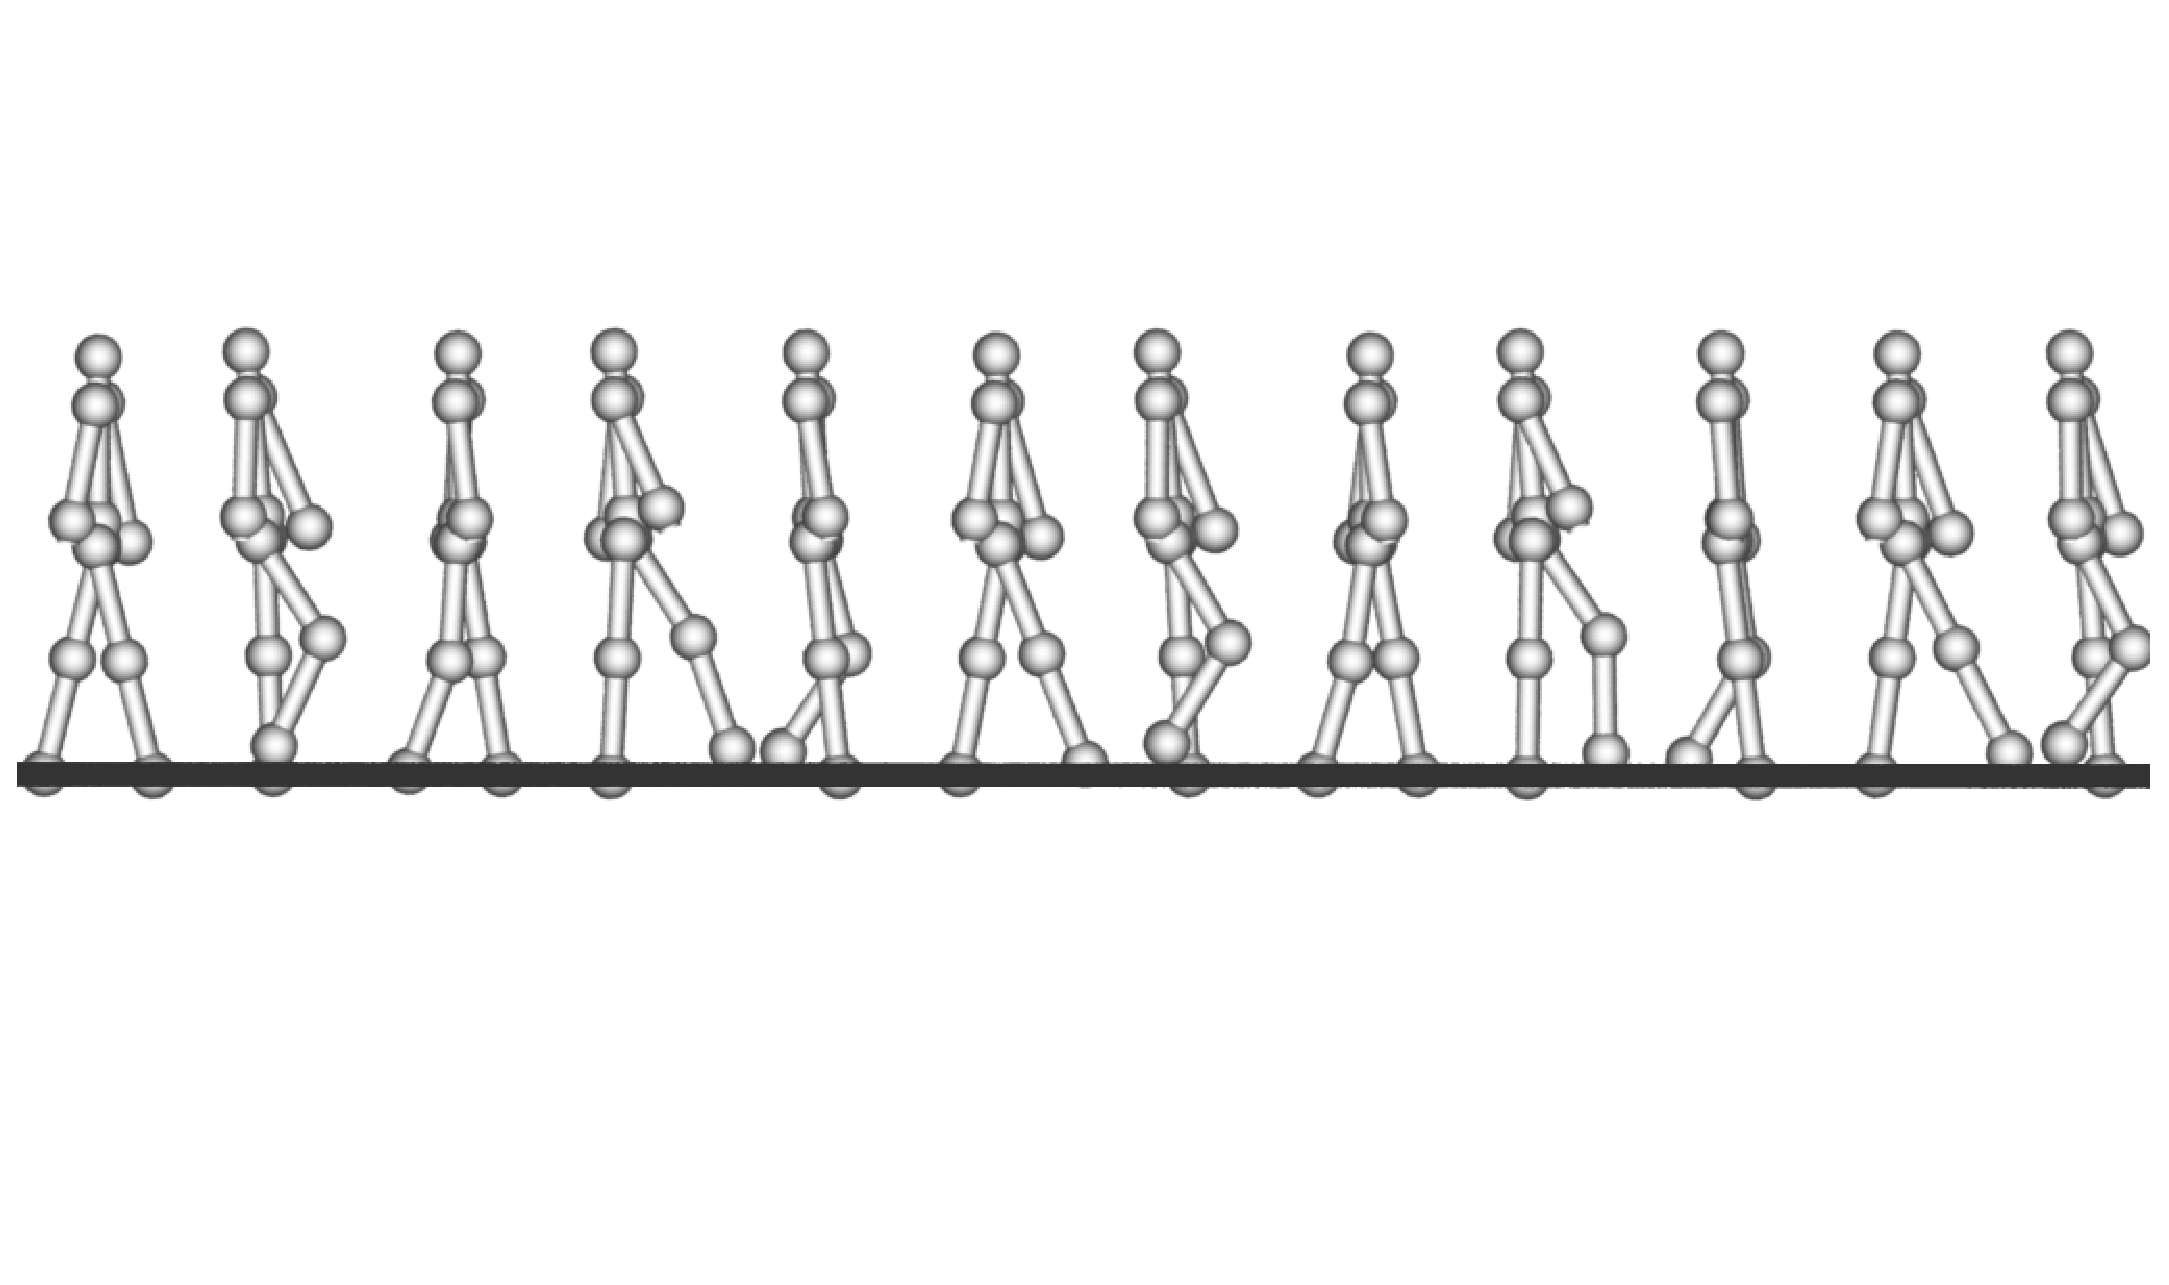
\includegraphics[width=0.7\textwidth]{stepsize4}
    \caption{gait with stepsize 4}
    \label{fig:ssp3}
\end{center}
\end{figure}







\subsection{Varying Slopes}
Neural Oscillator can maintain walking on varying slopes, but can't make character walk up slope.
Lie Group action allow the character to walk up a slope with a constant angle.
However varying the slope will result in walking failure.
Combining the two methods, the passive walker can walk varying up slope.


The control strategy is straight forward.
Lie group action is maintained on each plane, during slope transition, controller looks ahead and set the lie group action for to walking on the slope for the next step.
At transition, the state will move far away from the stable limit cycle, and need a few steps to converge to the limit circle.
This result in gait adjustment.
Sometimes, character will take a few small steps and increase it to normal steps.


Figure~\ref{fig:vp1} and Figure~\ref{fig:vp2} show the gaits on smooth slopes.
The phase plot of gaits of Figure~\ref{fig:vp1} is shown in Figure~\ref{fig:vp2phas} 

\begin{figure}[!htbp]
  \begin{center}
      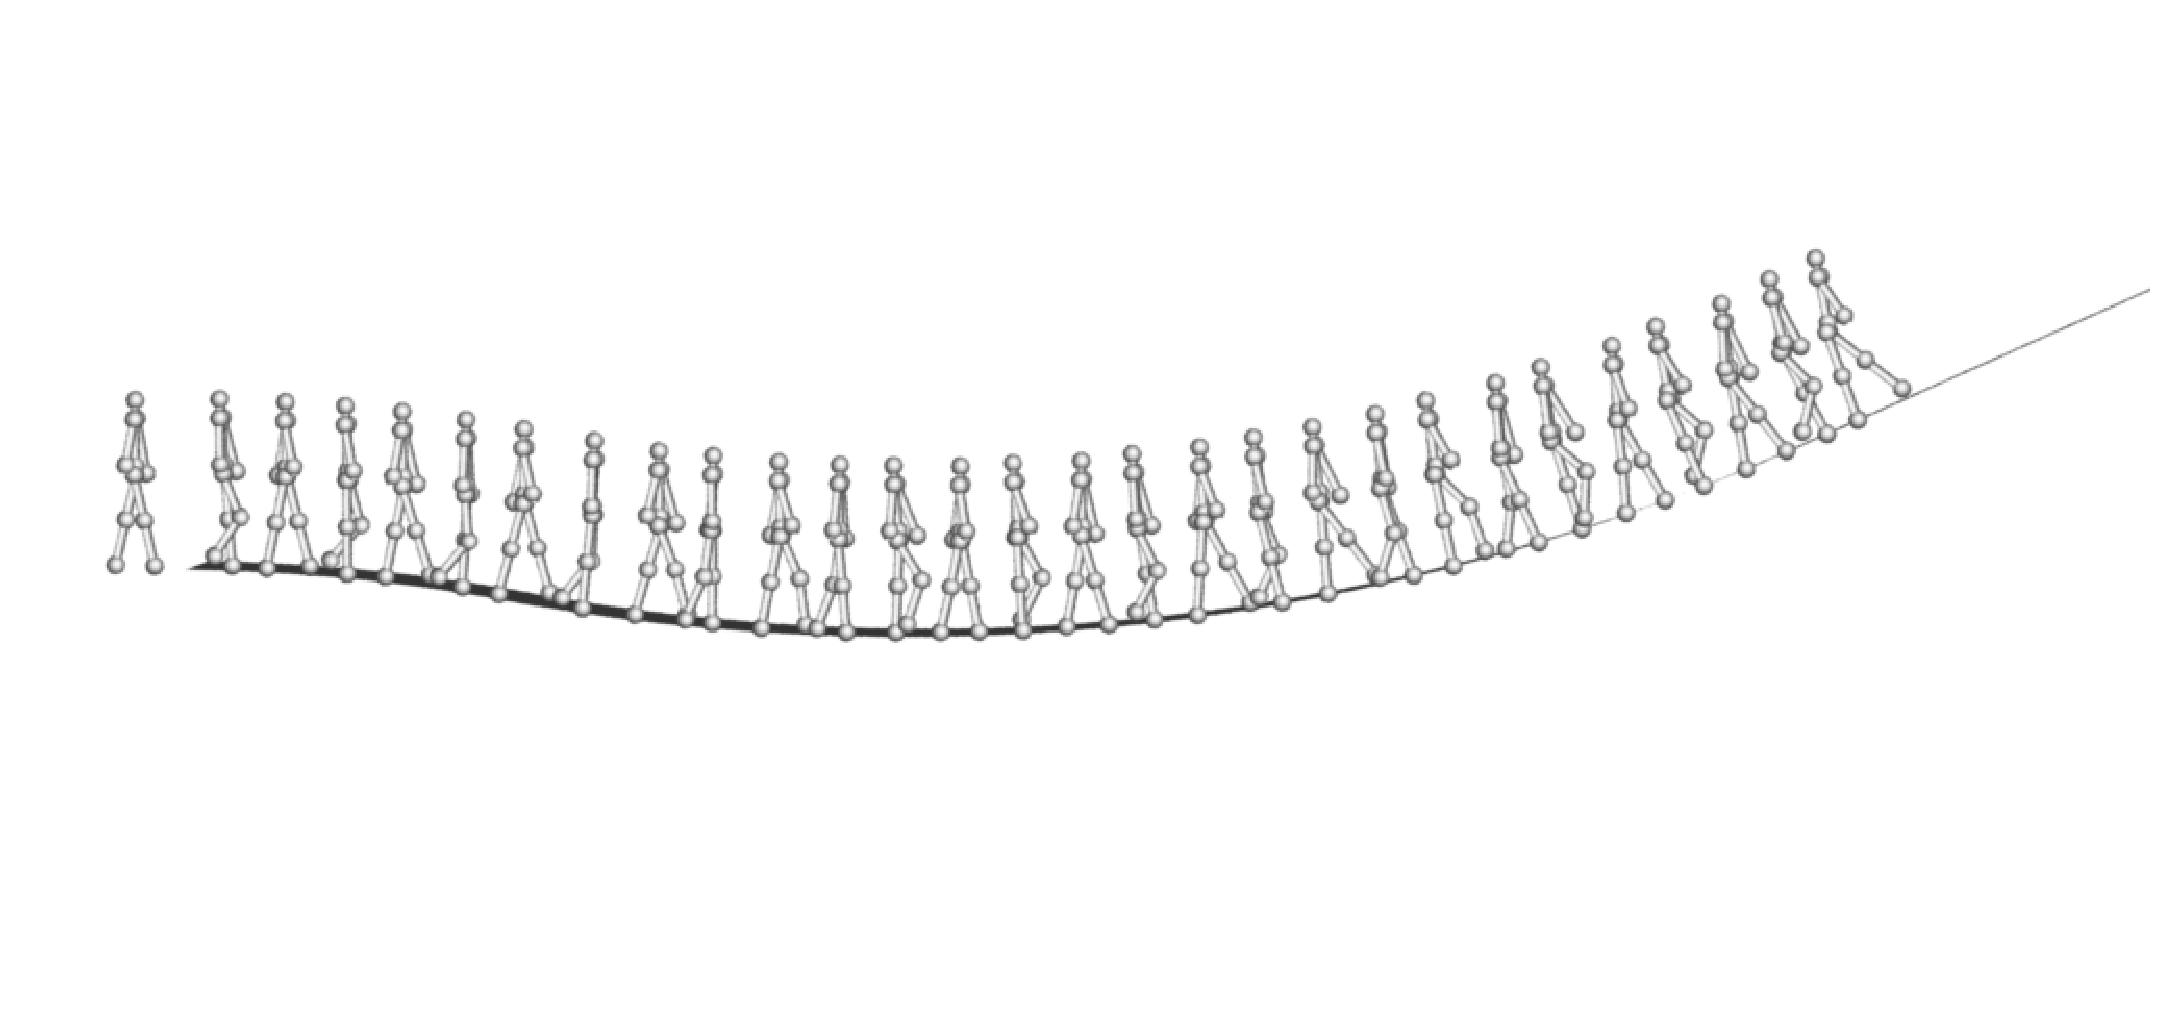
\includegraphics[width=0.7\textwidth]{vslope2}
    \caption{Continous Varying Slope}
    \label{fig:vp1}
\end{center}
\end{figure}


\begin{figure}[!htbp]
  \begin{center}
      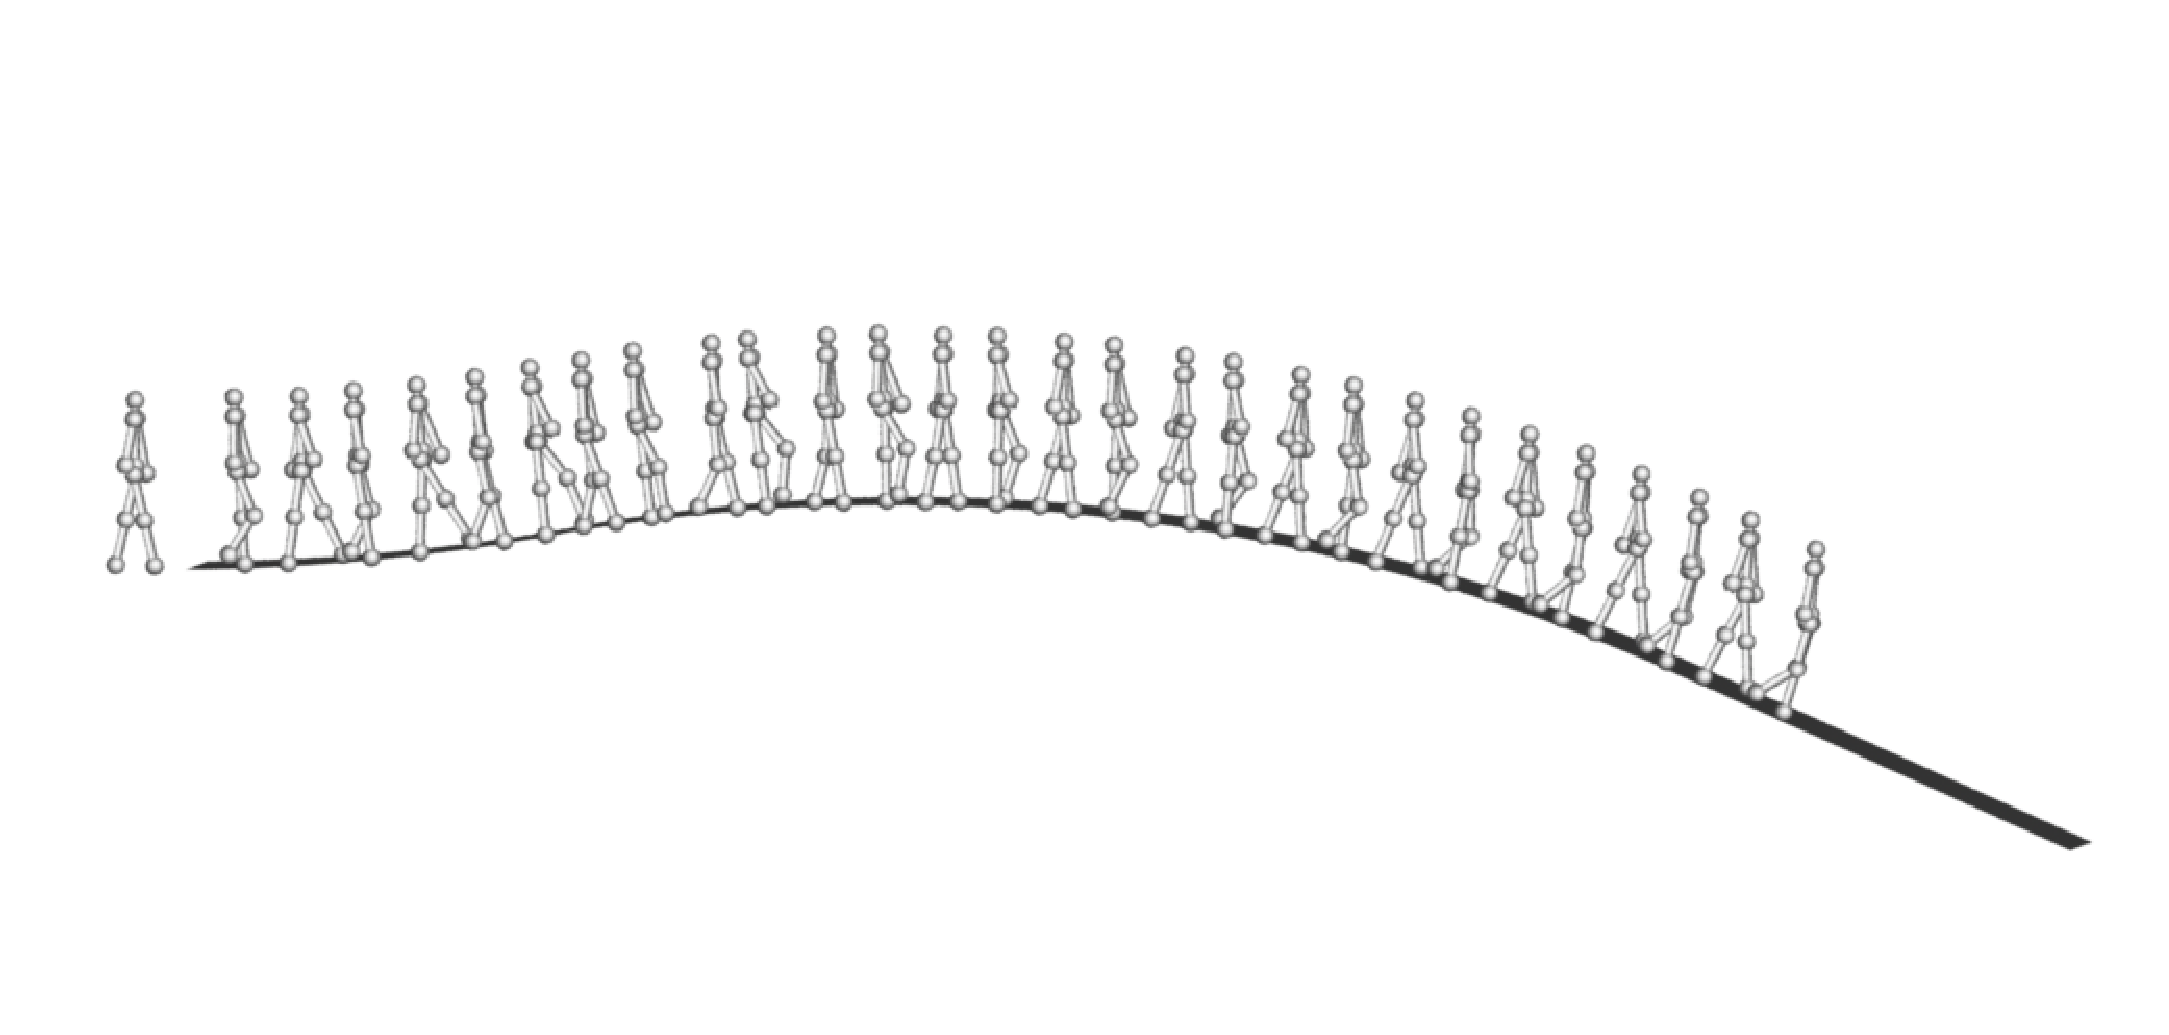
\includegraphics[width=0.7\textwidth]{vslope3}
    \caption{Continous Varying Slope}
    \label{fig:vp2}
\end{center}
\end{figure}


\begin{figure}[!htbp]
  \begin{center}
      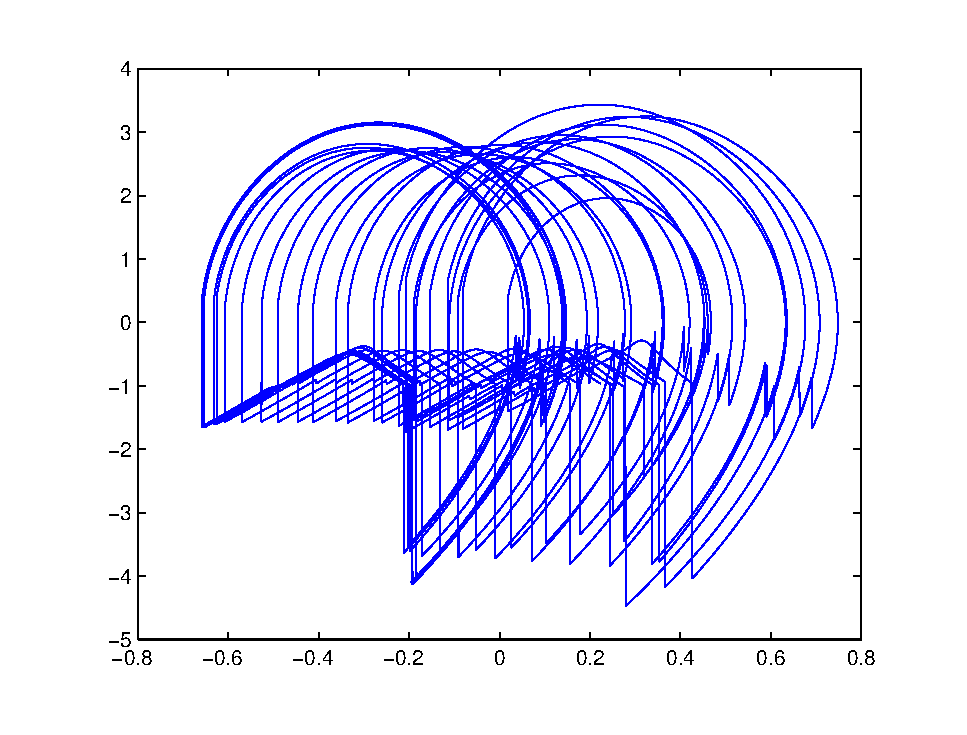
\includegraphics[width=0.7\textwidth]{vslope3phaseplot}
    \caption{Continous Varying Slope}
    \label{fig:vp2phas}
\end{center}
\end{figure}



Figure~\ref{fig:nonsmoothterrain1} and Figure~\ref{fig:nonsmootterrain2} show gaits on none smooth terrain.
Figure~\ref{fig:diffterrain2} shows the phase plot, where different colors show different slopes.
\begin{figure}[!htbp]
  \begin{center}
      \includegraphics[width=0.7\textwidth]{terrain2}
    \caption{Nonsmooth Terrain }
    \label{fig:nonsmoothterrain1}
\end{center}
\end{figure}

\begin{figure}[!htbp]
  \begin{center}
      \includegraphics[width=0.7\textwidth]{terrain3}
    \caption{Nonsmooth Terrain coloured}
    \label{fig:nonsmootterrain2}
\end{center}
\end{figure}


\begin{figure}[!htbp]
  \begin{center}
    \includegraphics[width=0.7\textwidth]{Terrain3PhaseDifferentColor}
    \caption{The Phase Plot of nonsmooth terrain}
    \label{fig:diffterrain2}
\end{center}
\end{figure}






